\chapter{Desarrollo hardware del manipulador}
\label{cap:capitulo5}
\begin{flushright}
  \begin{minipage}[]{10cm}
  \emph{La simplicidad es la máxima sofisticación}\\
  \end{minipage}\\
  Leonardo da Vinci\\
  \end{flushright}

\vspace{1cm}

\noindent En este capítulo, se describe el proceso de desarrollo completo llevado a cabo desde la concepción inicial de la 
idea hasta la materialización de un brazo robótico completamente funcional. A lo largo de estas páginas, se desglosará cada 
paso realizado y las dificultades encontradas, así como sus soluciones. 
\section{Geometría del manipulador}
\label{sec:eligiendo_geometría}
\noindent En esta sección se detalla el proceso llevado a cabo para definir el concepto y forma del robot, en base a 
los requisitos propuestos en el Capítulo \ref{cap:capitulo3}. 

Primeramente, se debe escoger el número de grados de libertad\footnote{número de movimientos independientes que puede realizar} del manipulador. 
En relación al espacio tridimensional (Figura \ref{fig:espacio_tridimensional}), este cuenta con 6, estando 3 de ellos ligados al 
posicionamiento (X, Y, Z) y los otros 3 a las orientaciones (RX, RY, RZ). Es por esto que 3 es el mínimo número de grados de libertad necesarios 
para poder posicionar el extremo del robot un punto cualquiera del espacio.

\begin{figure} [ht!]
  \begin{center}
    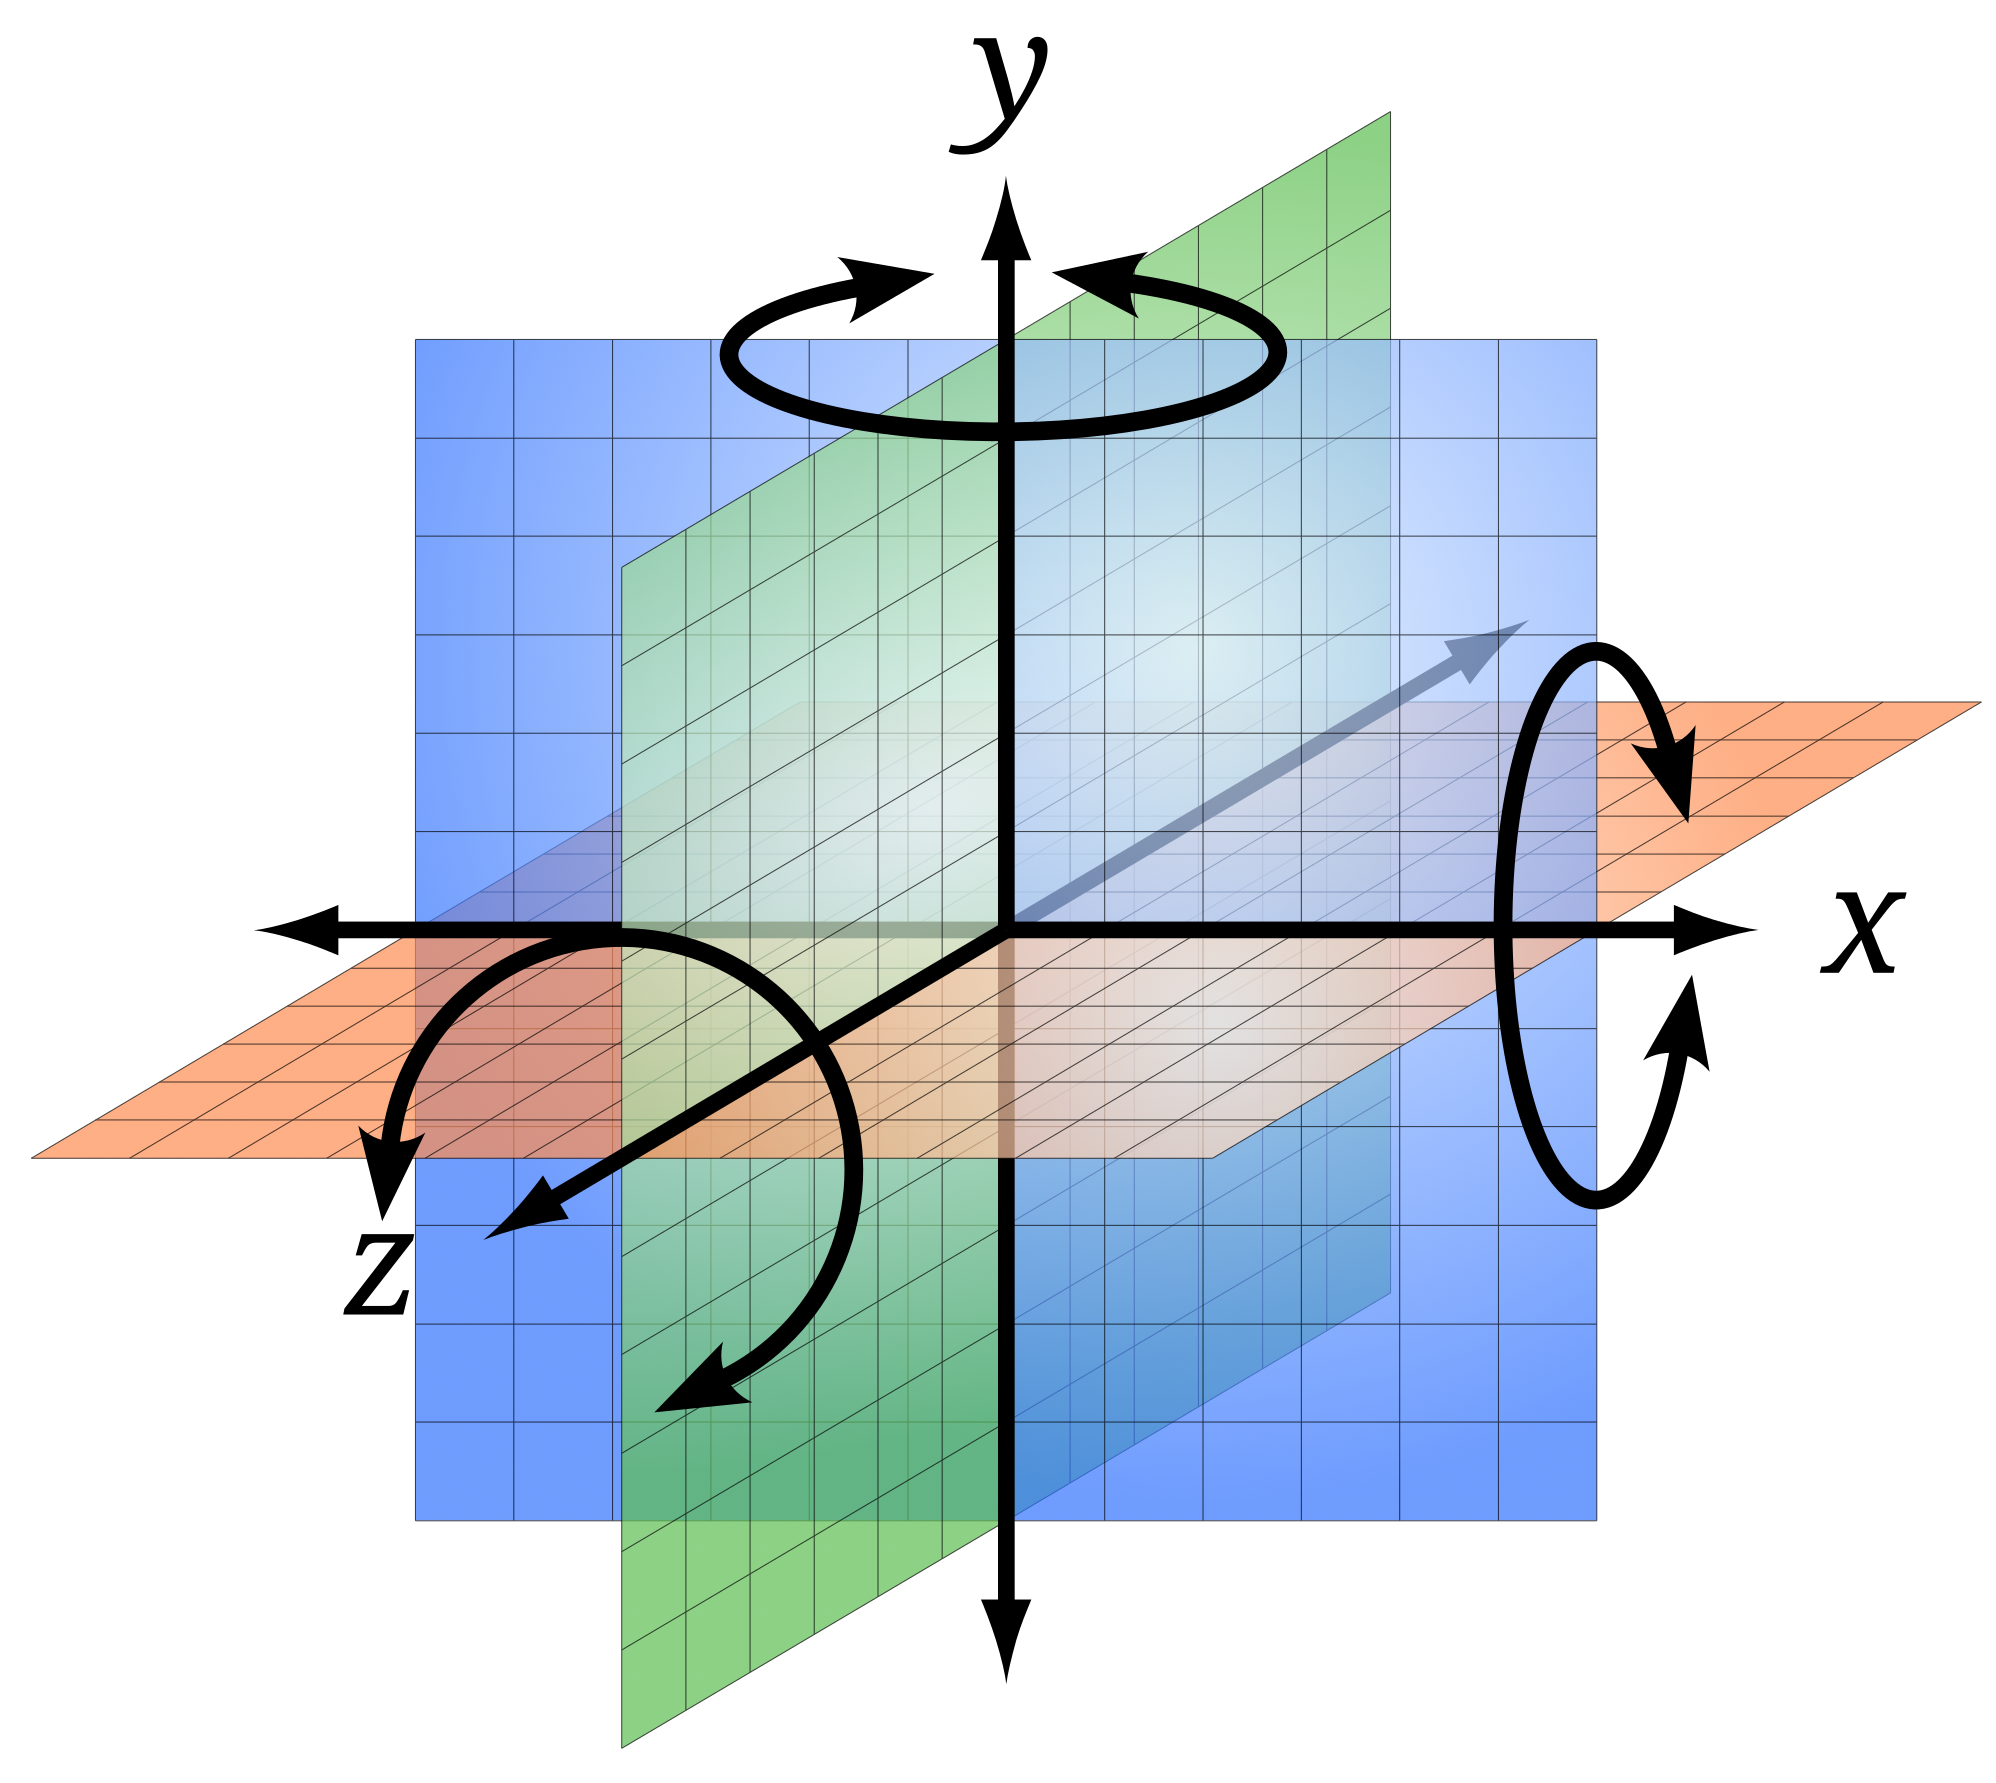
\includegraphics[width=4.8cm]{figs/coordinates.png}
  \end{center}
  \caption{Espacio tridimensional}
  \label{fig:espacio_tridimensional}
\end{figure}\ 

Teniendo esto en cuenta, se ha optado por usar ese número, y no uno mayor, debido a que esto encarecería los costes totales del robot, no pudiendo cumplir así 
los requisitos 1 y 5 que limitan en cuanto a precio y complejidad. 

Seguidamente, se debe elegir el tipo de articulación a utilizar. Aunque en robótica existen varias, en la práctica destacan dos:
\begin{itemize}
\item Revolución: Permite el movimiento de rotación alrededor de un eje fijo.
\item Prismático: Las partes del robot se pueden desplazar linealmente a lo largo de un eje específico. 

\begin{figure} [h!]
  \centering    
  \subfigure[Revolución]{\label{fig:j_rot}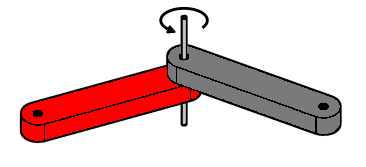
\includegraphics[width=0.4\linewidth ]{figs/joint_rot.png}}
  \hspace{1cm}
  \subfigure[Prismática]{\label{fig:j_prism}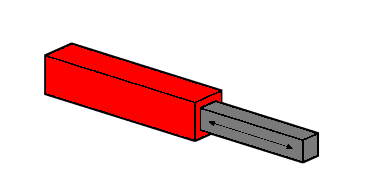
\includegraphics[width=0.4\linewidth]{figs/joint_prism.png}}
  \caption{Tipos de articulaciones más usadas en robótica}
\end{figure}

\end{itemize}

Finalmente, se ha optado por emplear articulaciones de tipo revolución, debido a que son más sencillas de implementar y 
están constituidas por un menor número de partes.

En cuanto a la geometría del manipulador, se debe contar con la limitación existente a la hora de tener únicamente 3 grados de libertad. Esta es 
que, aunque podemos alcanzar cualquier punto del espacio, no podemos controlar la orientación del extremo del robot en dicho punto. En base a esto, 
se ha investigado en Internet qué tipos de robot existen con ese número de grados de libertad y como lo solventan. Principalmente destacan dos 
soluciones: los robots SCARA y los robots basados en paralelogramos (presentados en la Sección \ref{sec:scara}). Ambos, tienen en común la 
característica de mantener su extremo siempre paralelo al suelo, por lo que se tiene conocimiento sobre 2 de las 3 orientaciones en ese punto. En 
la última orientación (Rotación en Z) se le suele incluir un cuarto grado de libertad, que en nuestro caso no tenemos. Aún así puede utilizarse con 
herramientas tipo electroimán o ventosas para tareas sencillas de movimiento de objetos.

Concretamente, se pretende implementar un robot basado en paralelogramos que utilice el mismo principio de funcionamiento que los utilizados en 
tareas de paletizado\footnote{Colocar objetos en un \textit{palet} de forma ordenada y eficiente}.

\section{Modelo alámbrico del manipulador}
\noindent El modelo alámbrico es una forma de analizar el movimiento de un sistema mecánico compuesto por ejes y eslabones. Este 
enfoque simplifica la representación visual al destacar las relaciones espaciales entre las diferentes partes del sistema mediante 
líneas y conexiones simbólicas.

En la Figura \ref{fig:mod_pinza_figure} se muestra un ejemplo creado específicamente para ilustrar este concepto.
\begin{figure} [ht!]
  \begin{center}
    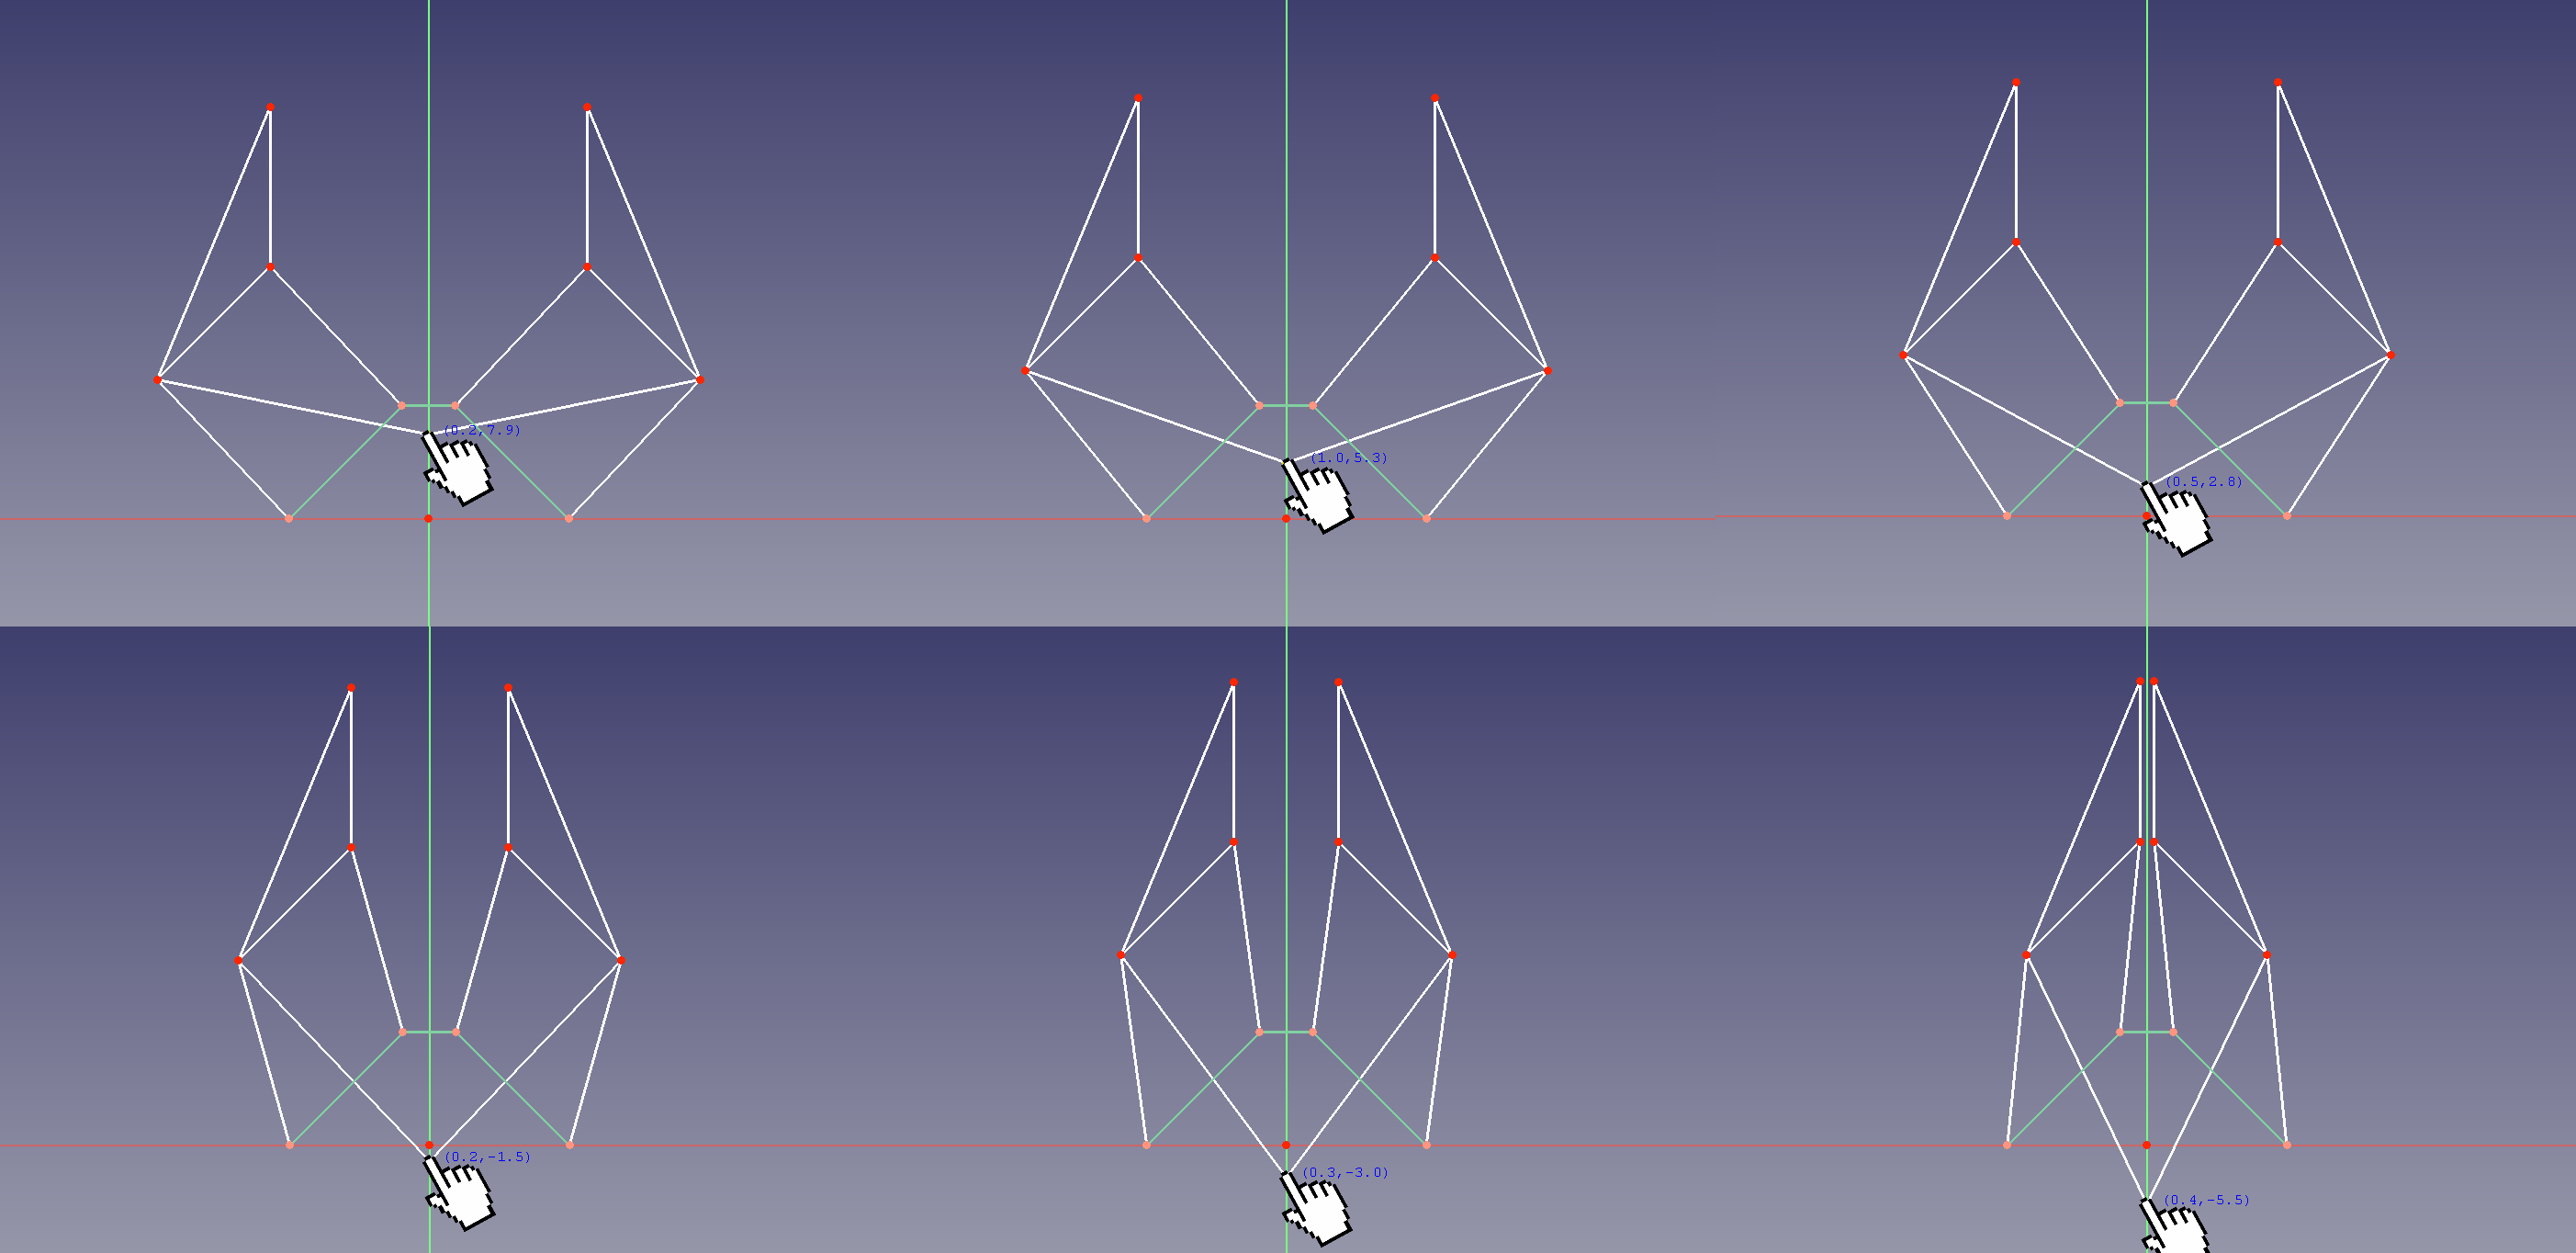
\includegraphics[width=15cm]{figs/pinza_evol.png}
  \end{center}
  \caption{Pinza paralela con 1 grado de libertad}
  \label{fig:mod_pinza_figure}
\end{figure}\ 

A la hora de crear el modelo alámbrico de este robot, se ha tomado como referencia el del robot 
casero MeArm (Figura \ref{fig:mearm}), en concreto el modelo alámbrico usado por Juan González en la asignatura de 
Mecatrónica\footnote{\url{https://github.com/myTeachingURJC/Mecatronica/wiki/S3:-Estructuras-mec\%C3\%A1nicas-(II)}} de esta Universidad.\\
\begin{figure} [ht!]
  \begin{center}
    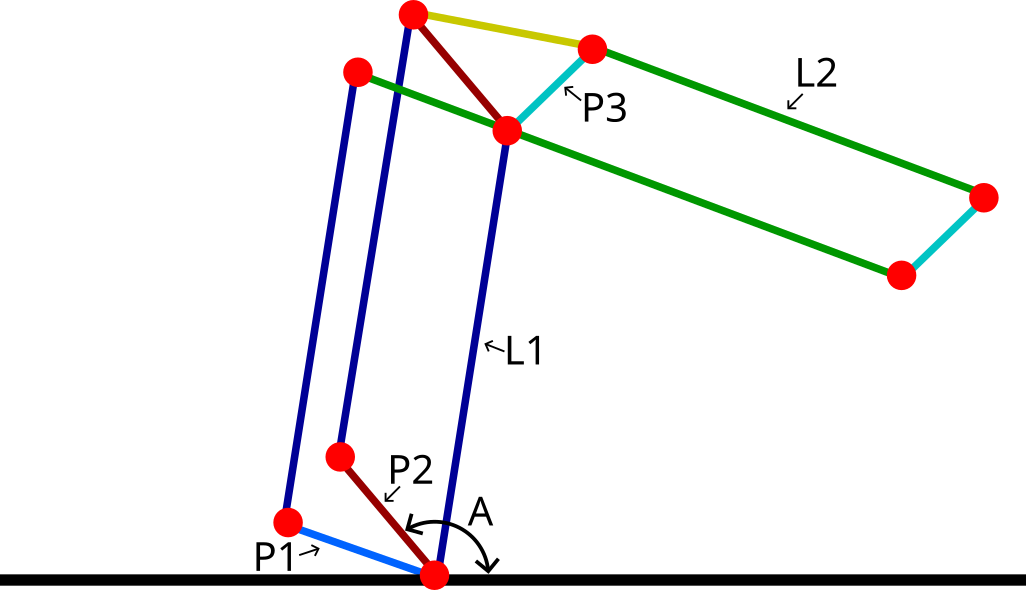
\includegraphics[width=15cm]{figs/mearm_params.png}
  \end{center}
  \caption{Principio fundamental del brazo MeArm}
  \label{fig:mearm_params}
\end{figure}\ 


Este robot está definido por una serie de parámetros a los que se les ha puesto nombre: L1, L2, P1, P2, P3 y A (mostrados 
en la Figura \ref{fig:mearm_params}). En función de los valores de estos parámetros, el comportamiento del brazo será diferente. Para 
encontrar los adecuados, no queda otra que utilizar la experimentación. Aún así, si se sigue un cierto orden, el proceso resulta realmente sencillo. 

\newpage
\noindent Es por esto que se ha seguido el siguiente procedimiento: 

\begin{enumerate}
\item Una manera de comenzar, es estableciendo el largo de los eslabones primarios L1 y L2. En base al tamaño de escritorio que se le pretende 
dar al robot, 17 centímetros por eslabón es un buen punto de partida.
\item El siguiente paso es elegir P1, P2 y P3. Estos son los lados cortos de los paralelogramos. Es importante jugar con estos valores 
de tal manera que se consiga obtener los más largos posibles y estos no intersequen entre sí. Esto es debido a que las piezas reales ocupan un cierto espacio y si el paralelogramo es 
muy pequeño no realizarán todo el recorrido ya que chocarán entre sí. 
\item El ángulo A restringe el paralelogramo que mantiene el extremo del robot paralelo al suelo. Este ángulo hay que variarlo ligeramente. Un buen 
punto de partida es 120º. Este valor es crítico ya que afecta significativamente a la accesibilidad del brazo a lugares próximos a su base. 
\end{enumerate}
\newpage
En la Figura \ref{fig:g_arm_alambrico} se muestra el modelo alámbrico final de este manipulador, bautizado como G-Arm\footnote{Bautizado así 
debido al lenguaje de programación que será utilizado posteriormente para comunicarse con él}:\\
\begin{figure} [ht!]
  \begin{center}
    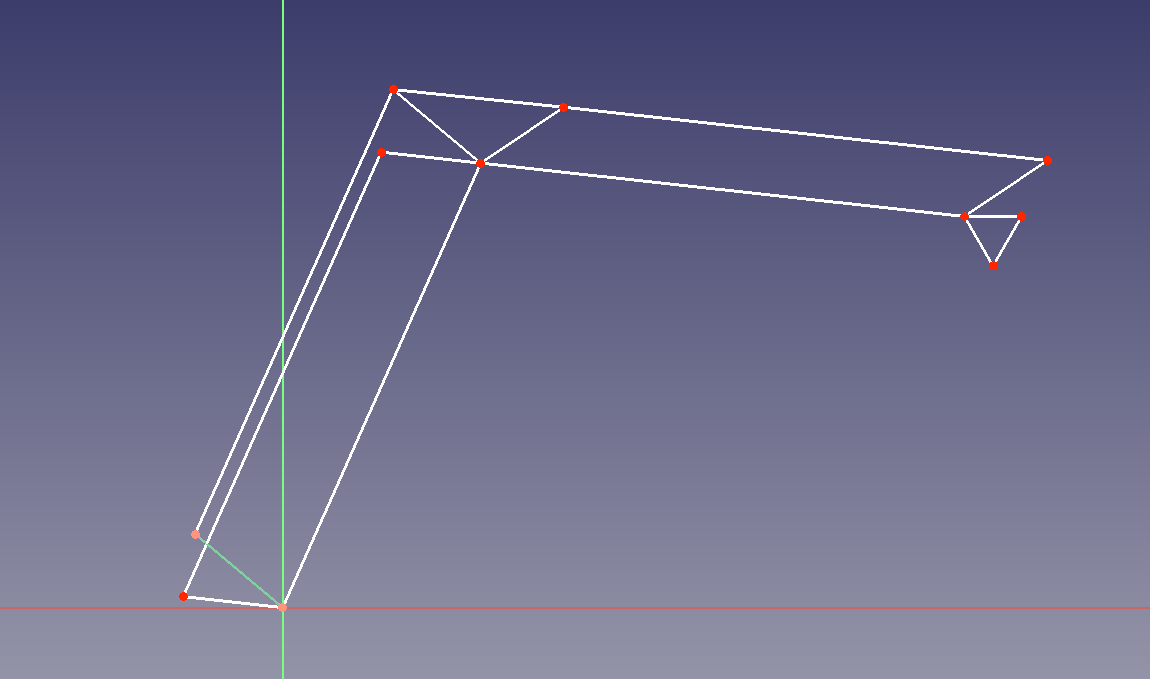
\includegraphics[width=15cm]{figs/alambrico_garm.png}
  \end{center}
  \caption{Modelo alámbrico de G-Arm}
  \label{fig:g_arm_alambrico}
\end{figure}\ 

Dando como resultado la siguiente tabla de parámetros:
\begin{table}[H]
\begin{center}
\begin{tabular}{|c|c|}
\hline
\textbf{Parámetros} & \textbf{Valores} \\
\hline
L1 & 170mm \\
L2 & 170mm \\
P1 & 35mm \\
P2 & 35mm \\
P3 & 25mm \\
A & 135º \\
\hline
\end{tabular}
\caption{Parámetros del modelo alámbrico de G-Arm}
\label{cuadro:parametros_alambrico}
\end{center}
\end{table}
\newpage
\section{Bocetos}
\noindent Realizar bocetos es una fase clave del diseño que se lleva a cabo antes de comenzar a modelar en 3D. Con ellos, se busca tener una idea 
clara de la forma 
y posición de los elementos que constituyen el robot.  
Para el desarrollo de este brazo, se han realizado numerosos bocetos, de los cuales se conservan aquellos dibujados digitalmente en 
un iPad. En la Figura \ref{fig:bocetos} se muestran algunos de ellos.

\begin{figure} [h!]
  \centering    
  \subfigure[]{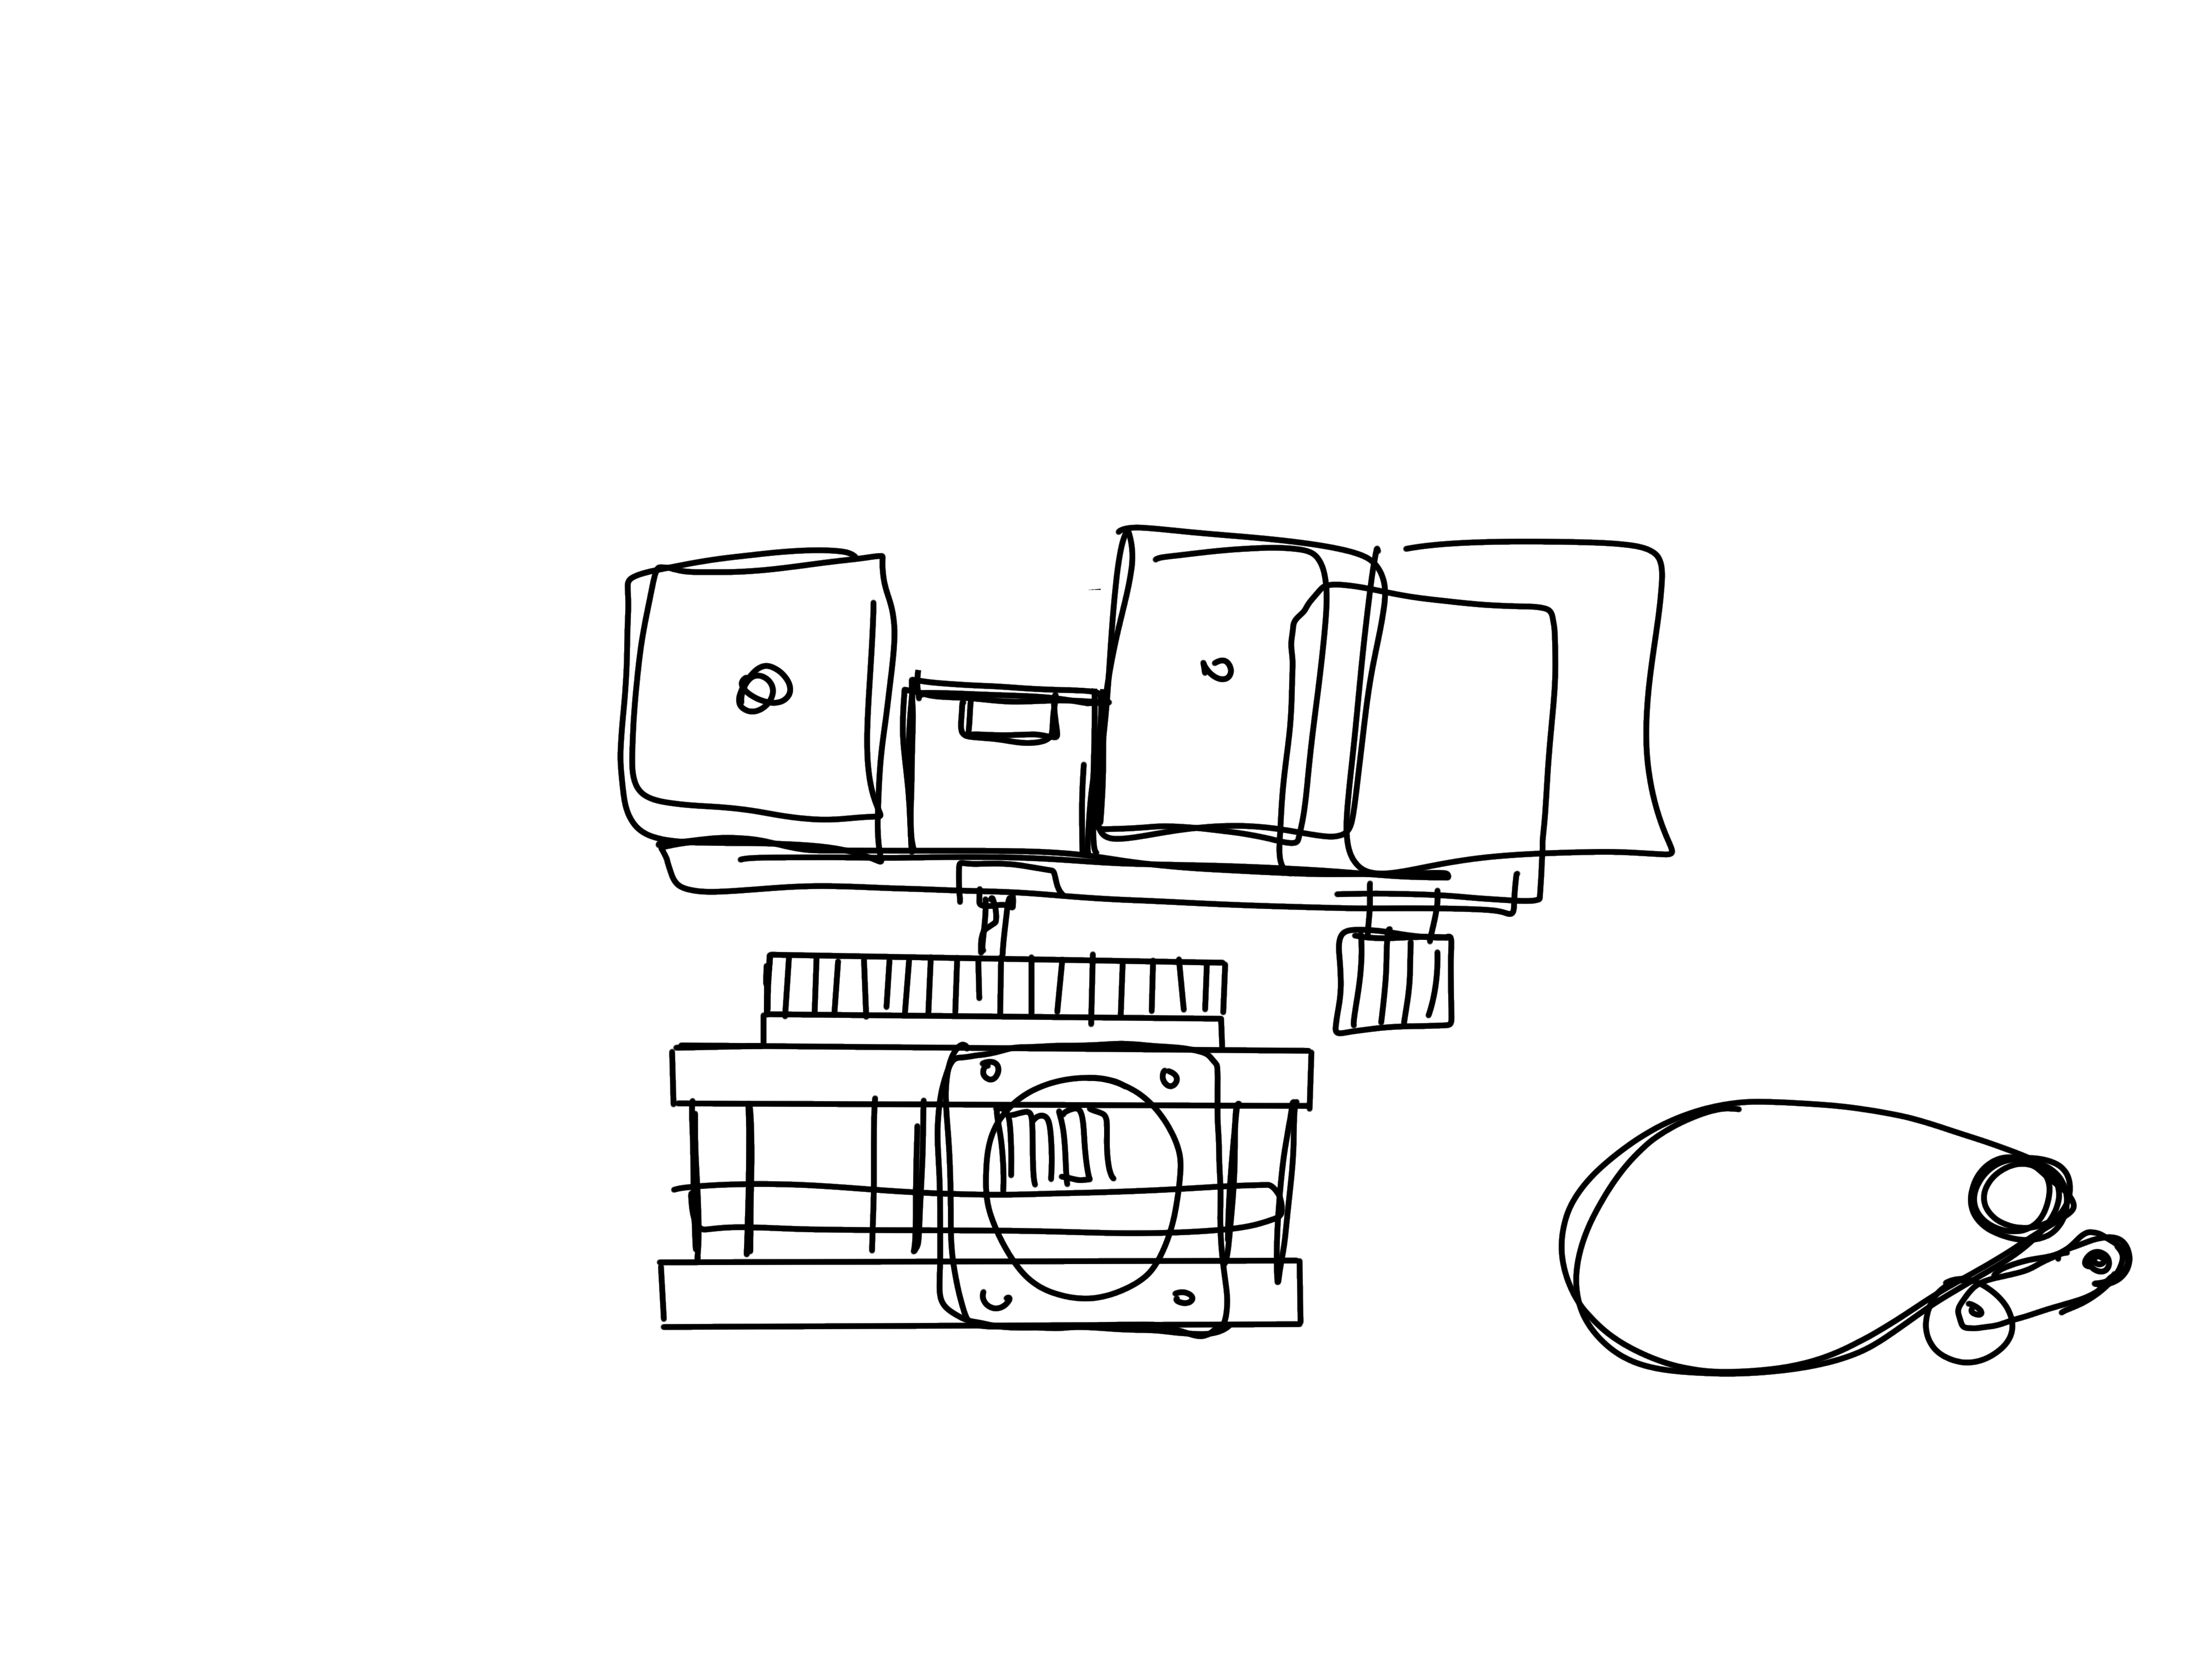
\includegraphics[width=0.5\linewidth ]{figs/boceto5.png}}
  \hspace{1cm}
  \subfigure[]{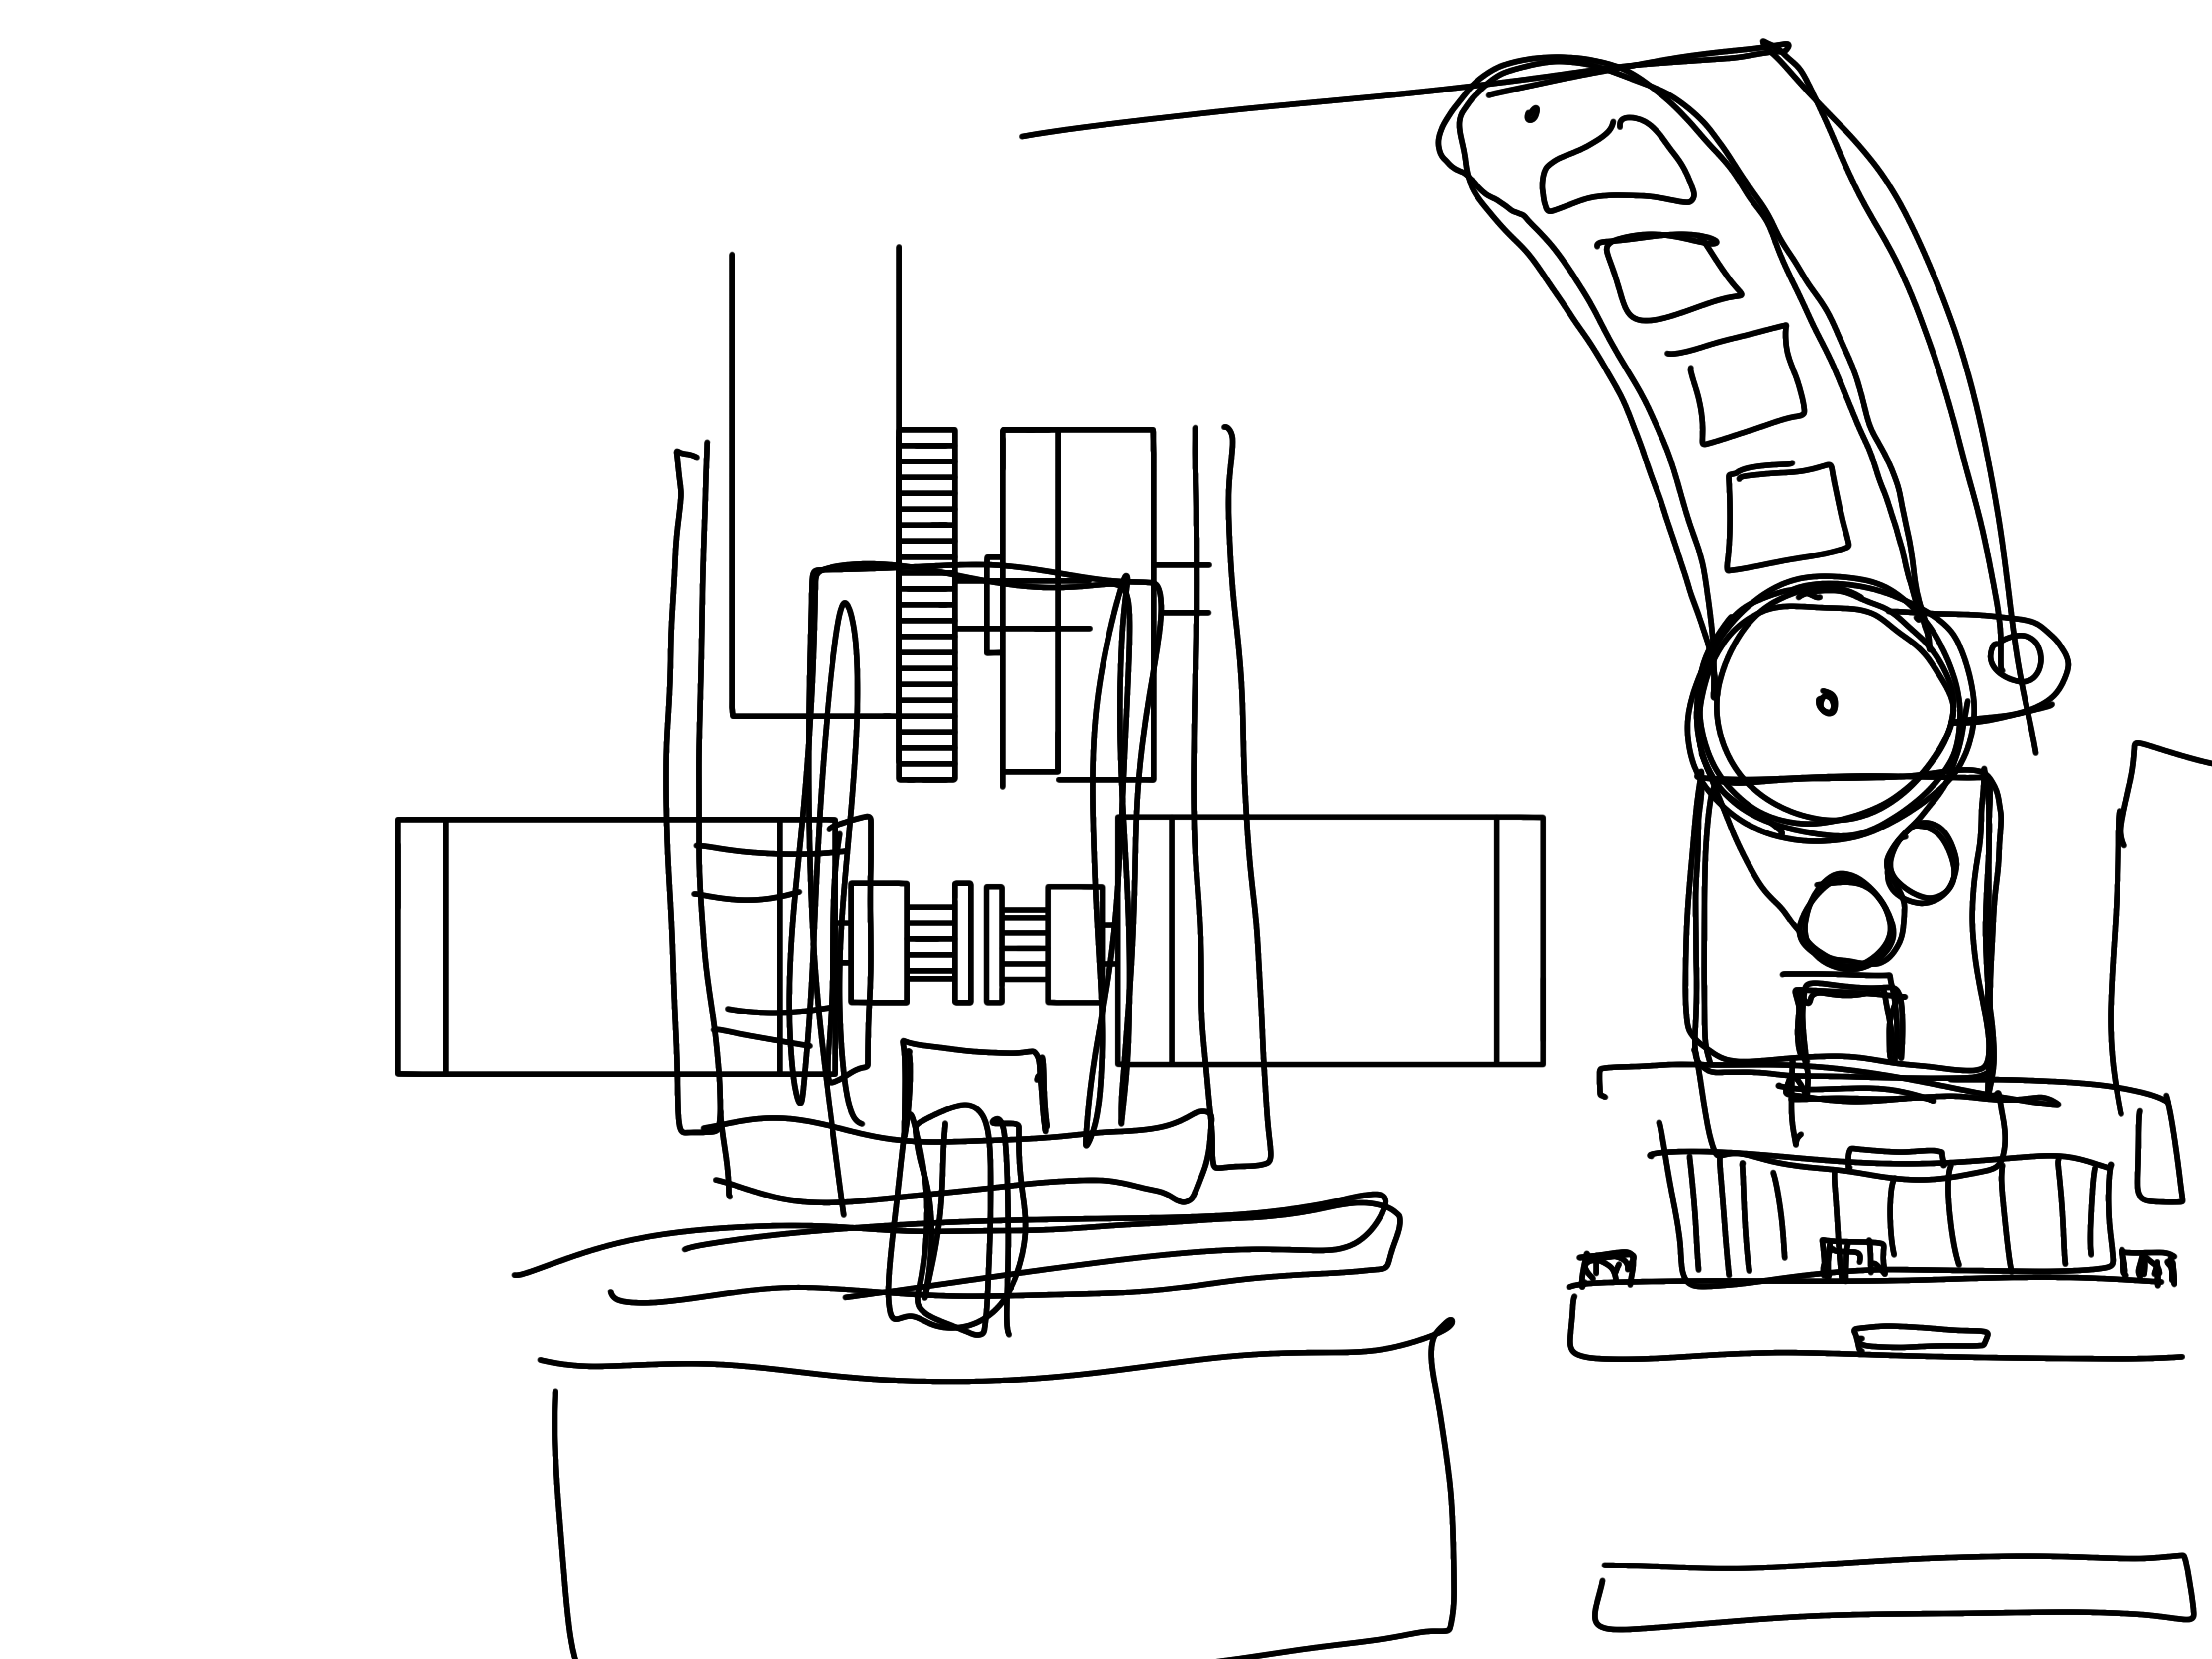
\includegraphics[width=0.4\linewidth]{figs/boceto2.png}}
  \subfigure[]{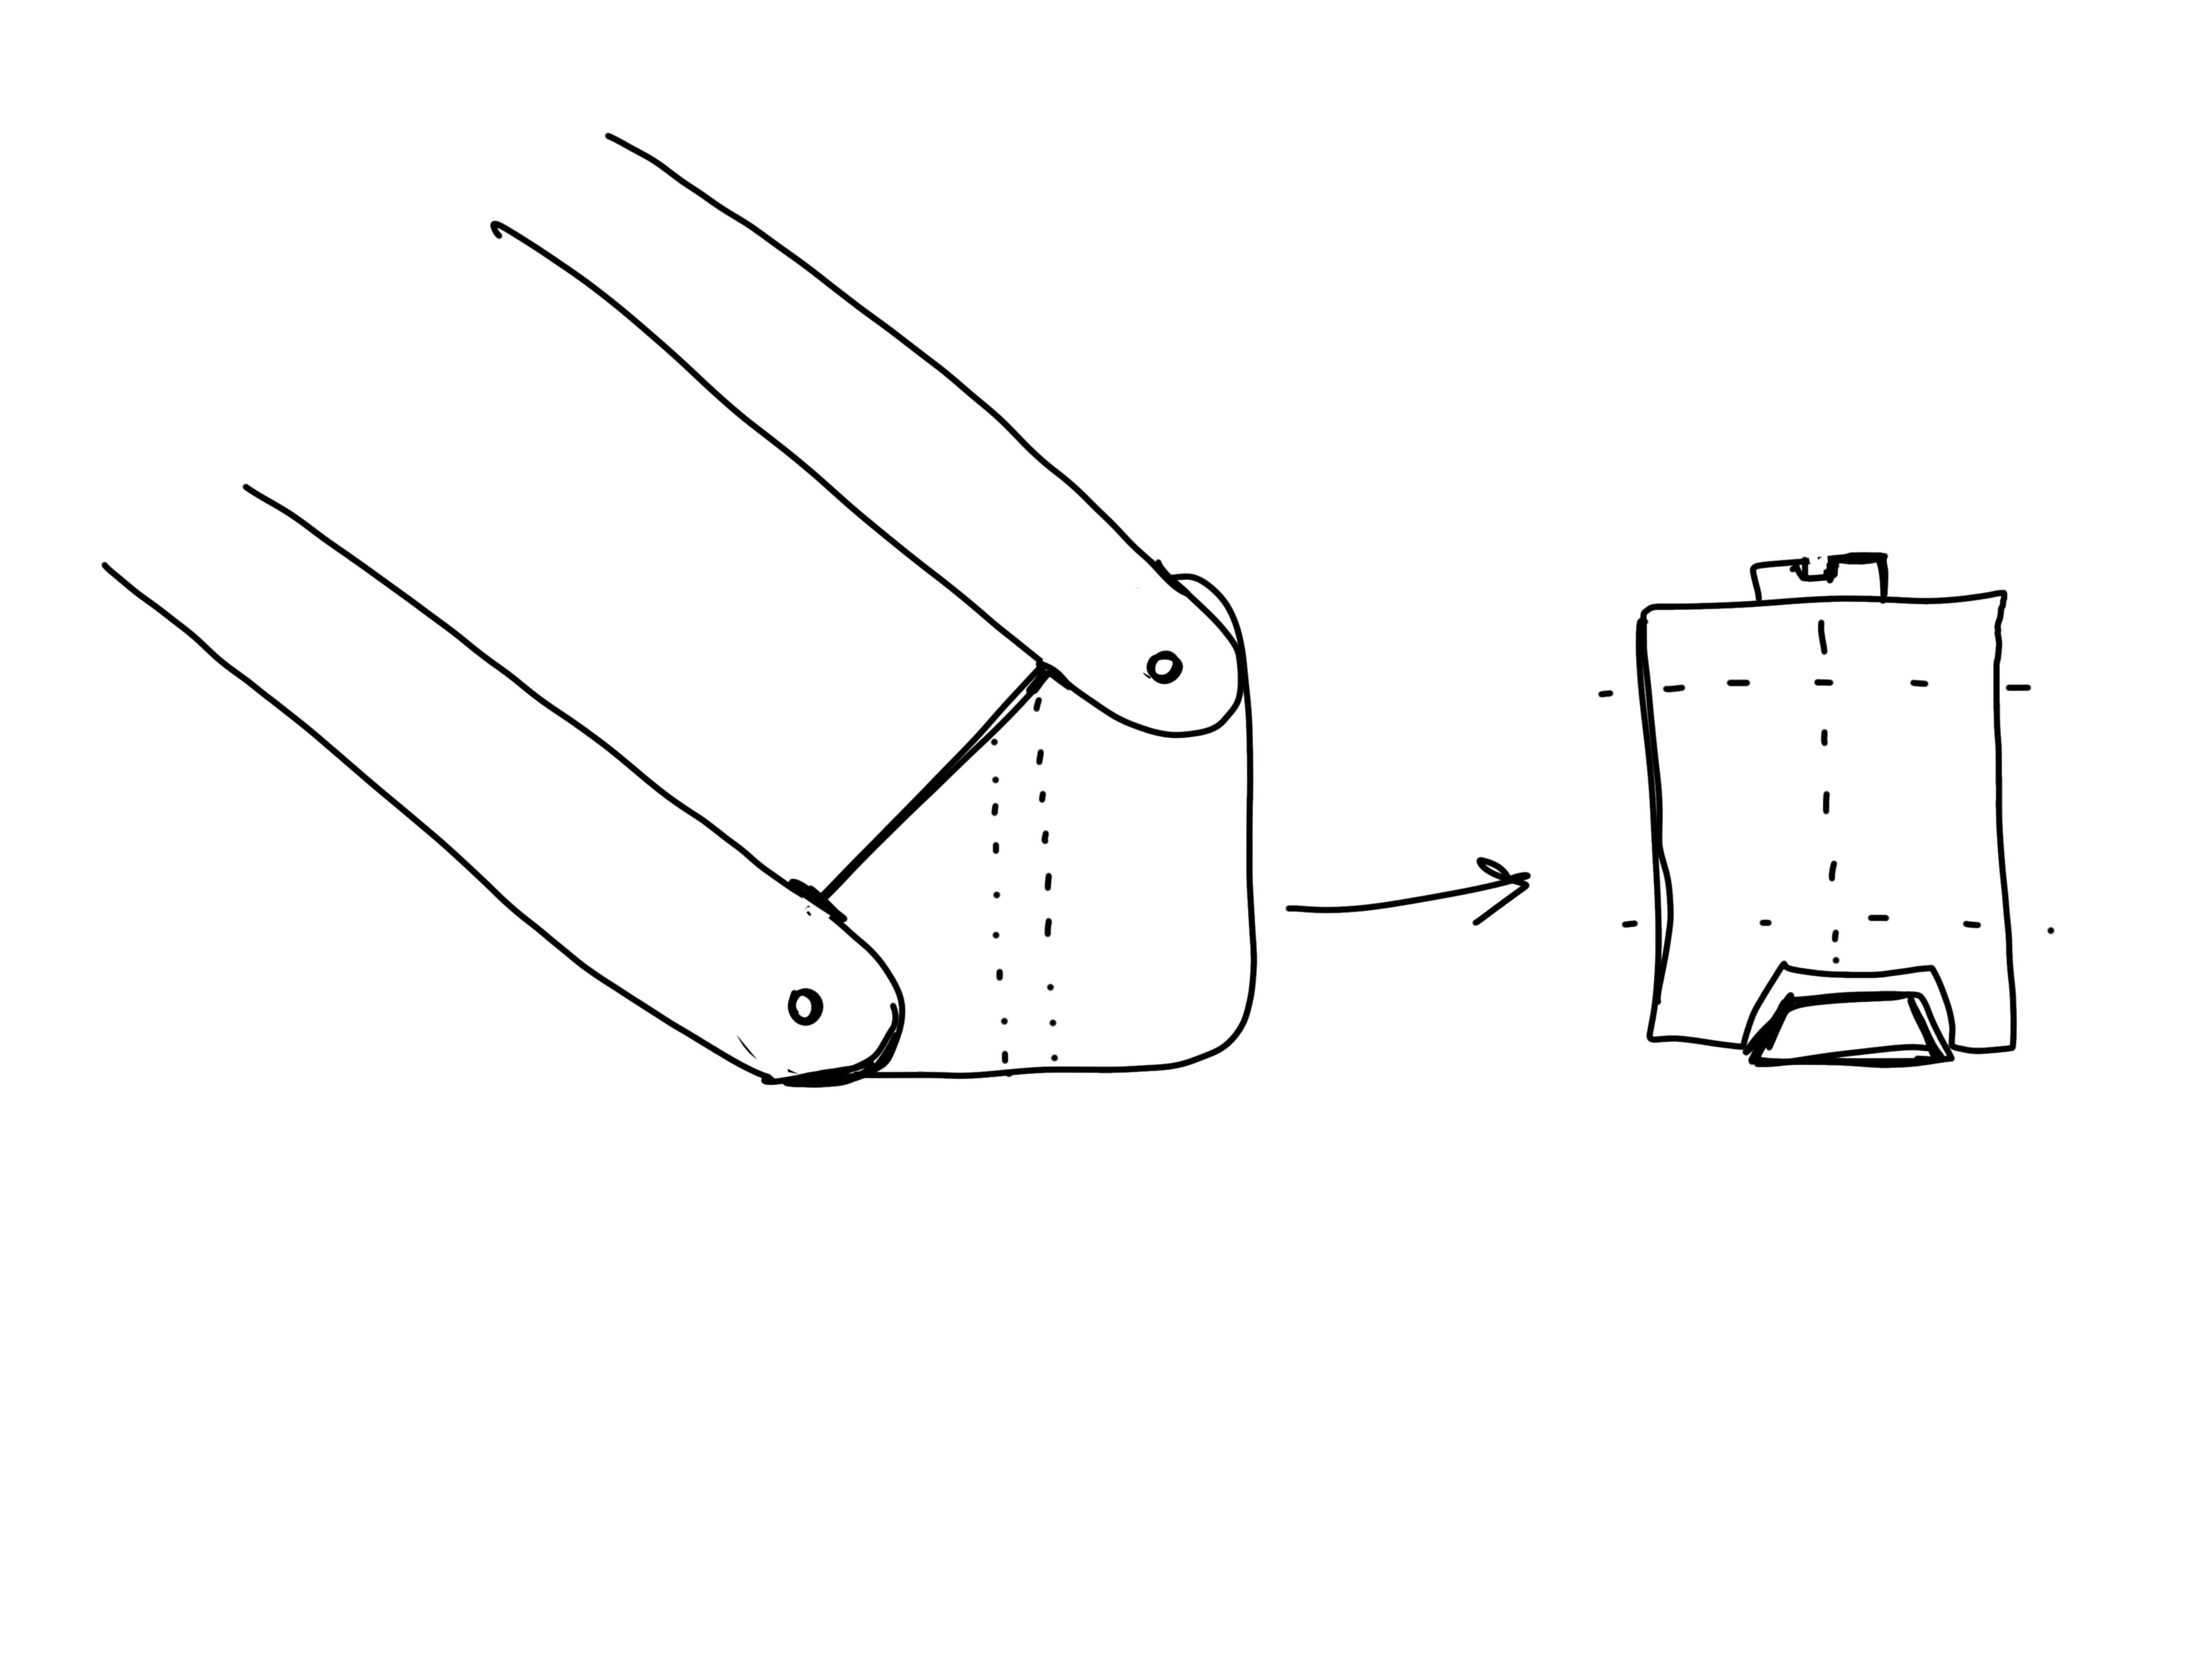
\includegraphics[width=0.4\linewidth ]{figs/boceto8.jpeg}}
  \hspace{1cm}
  \subfigure[]{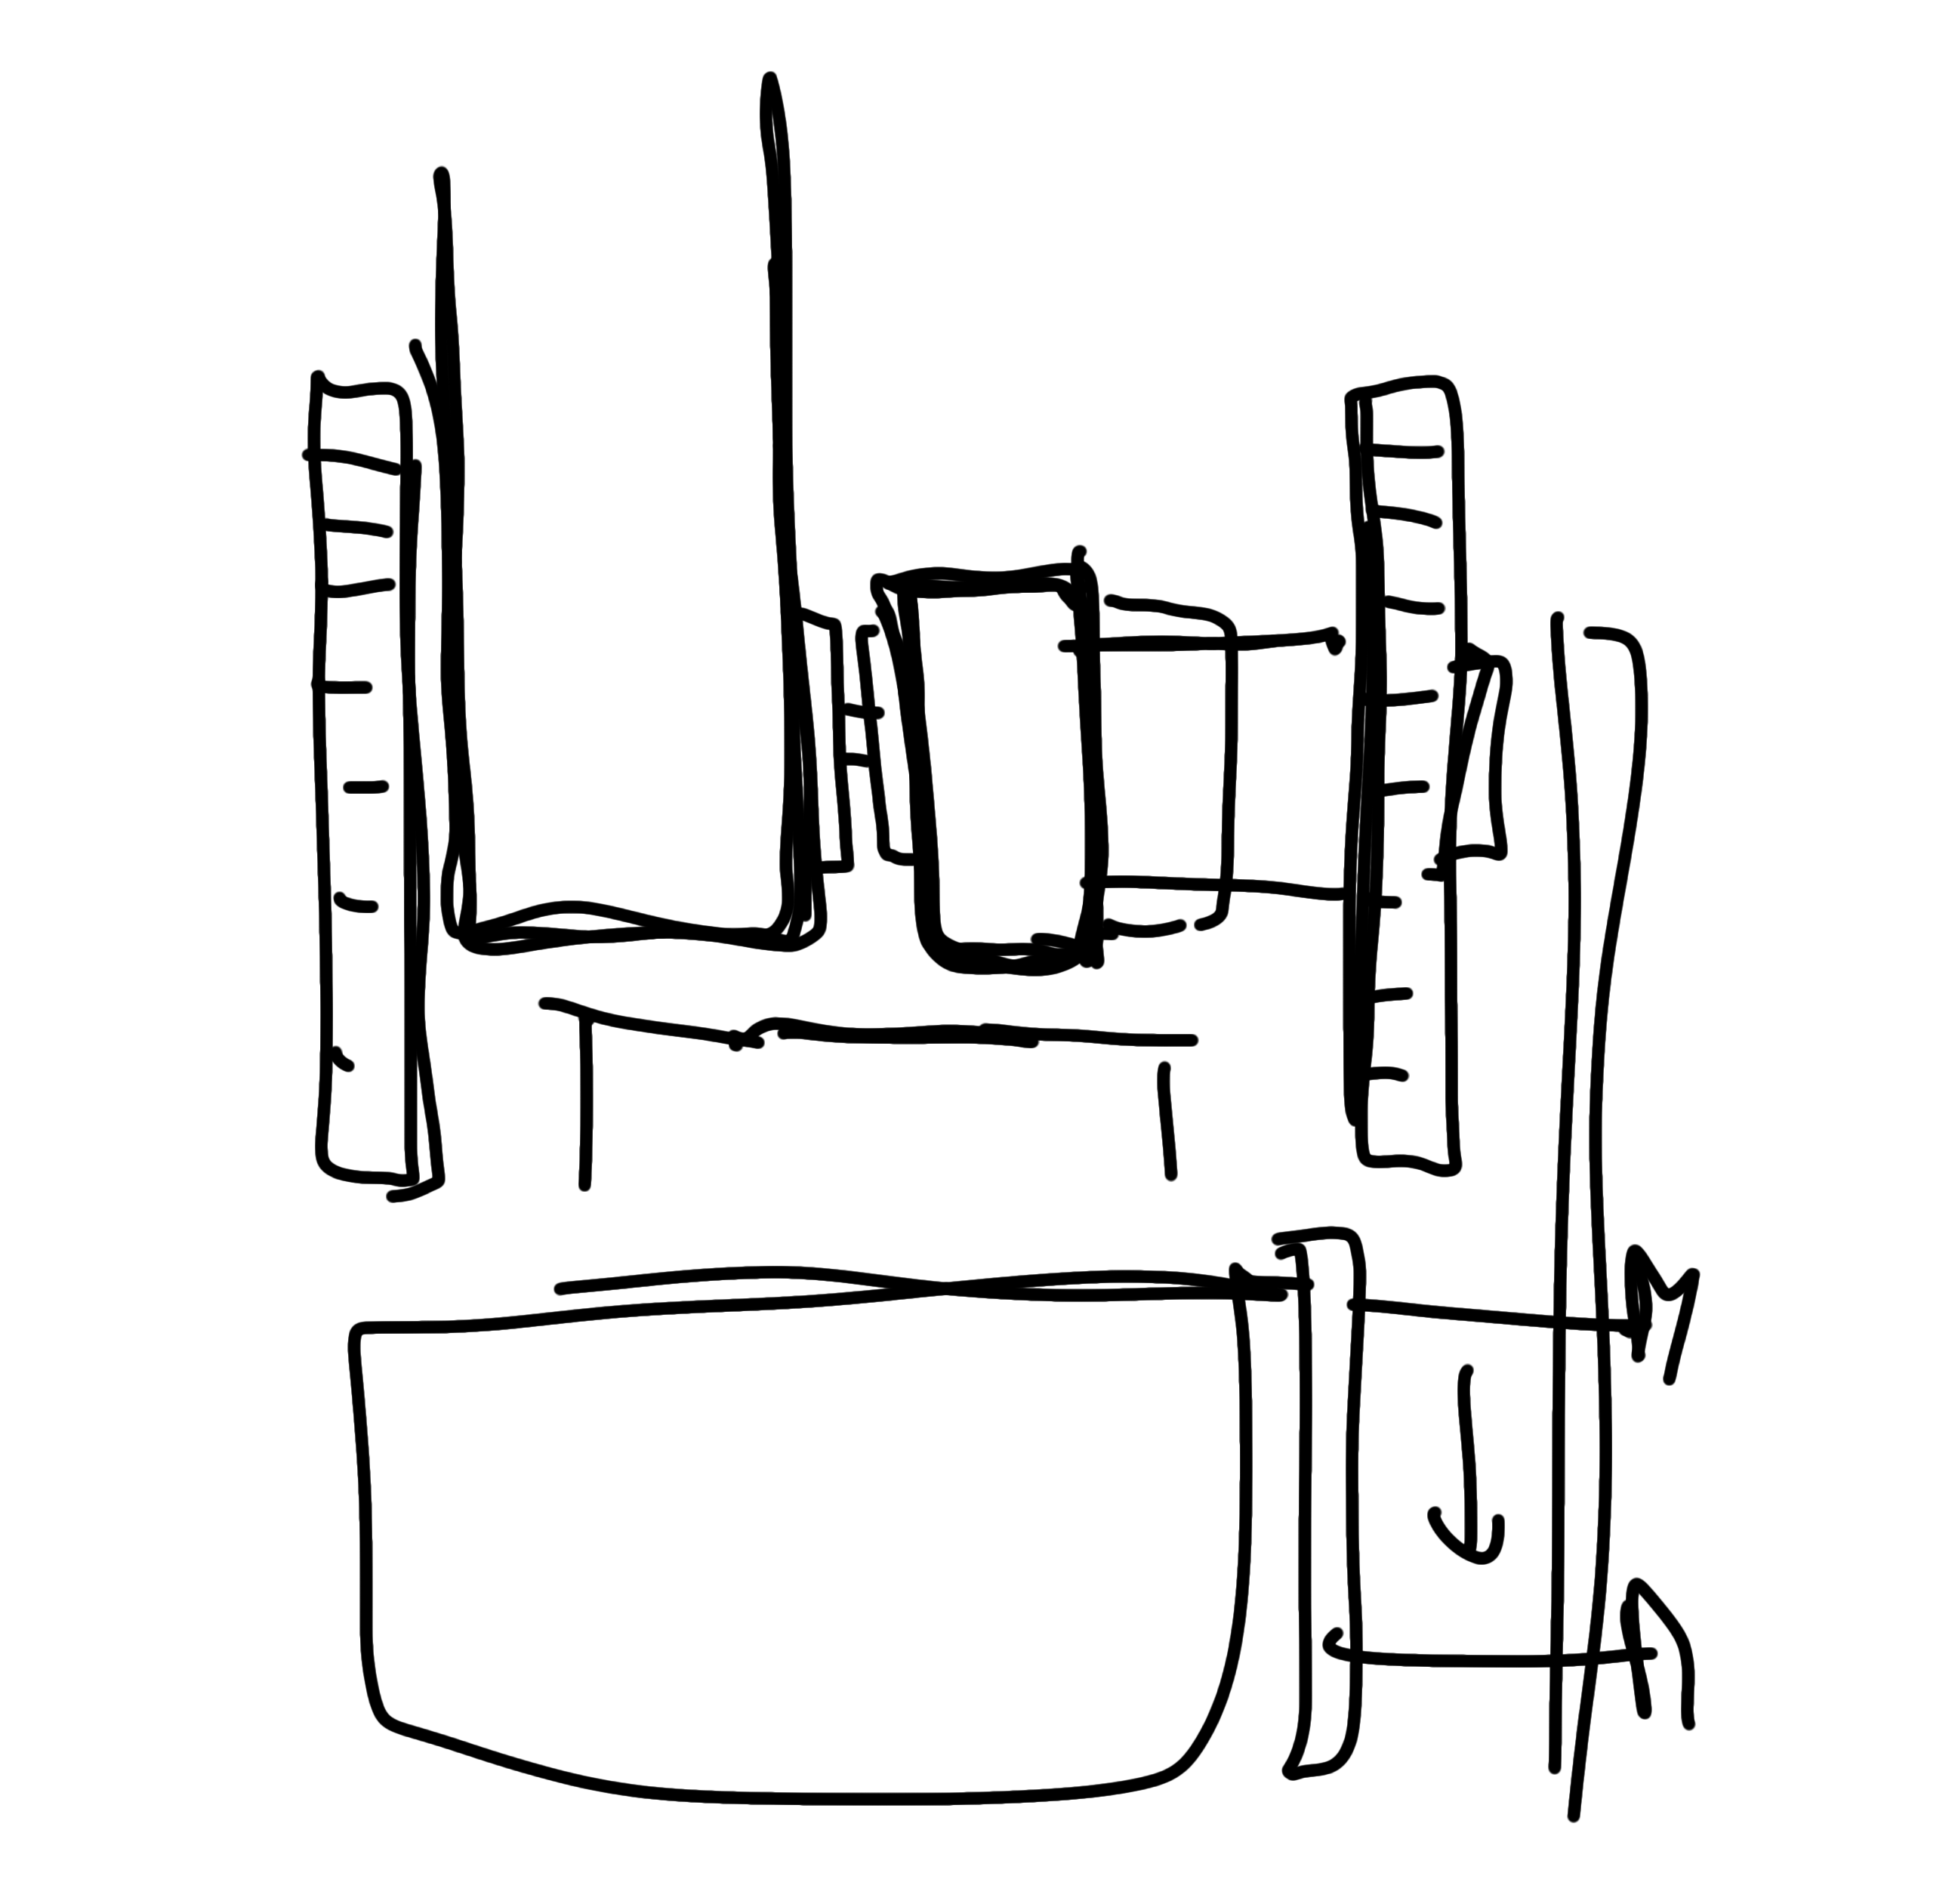
\includegraphics[width=0.4\linewidth]{figs/boceto4.png}}
  \subfigure[]{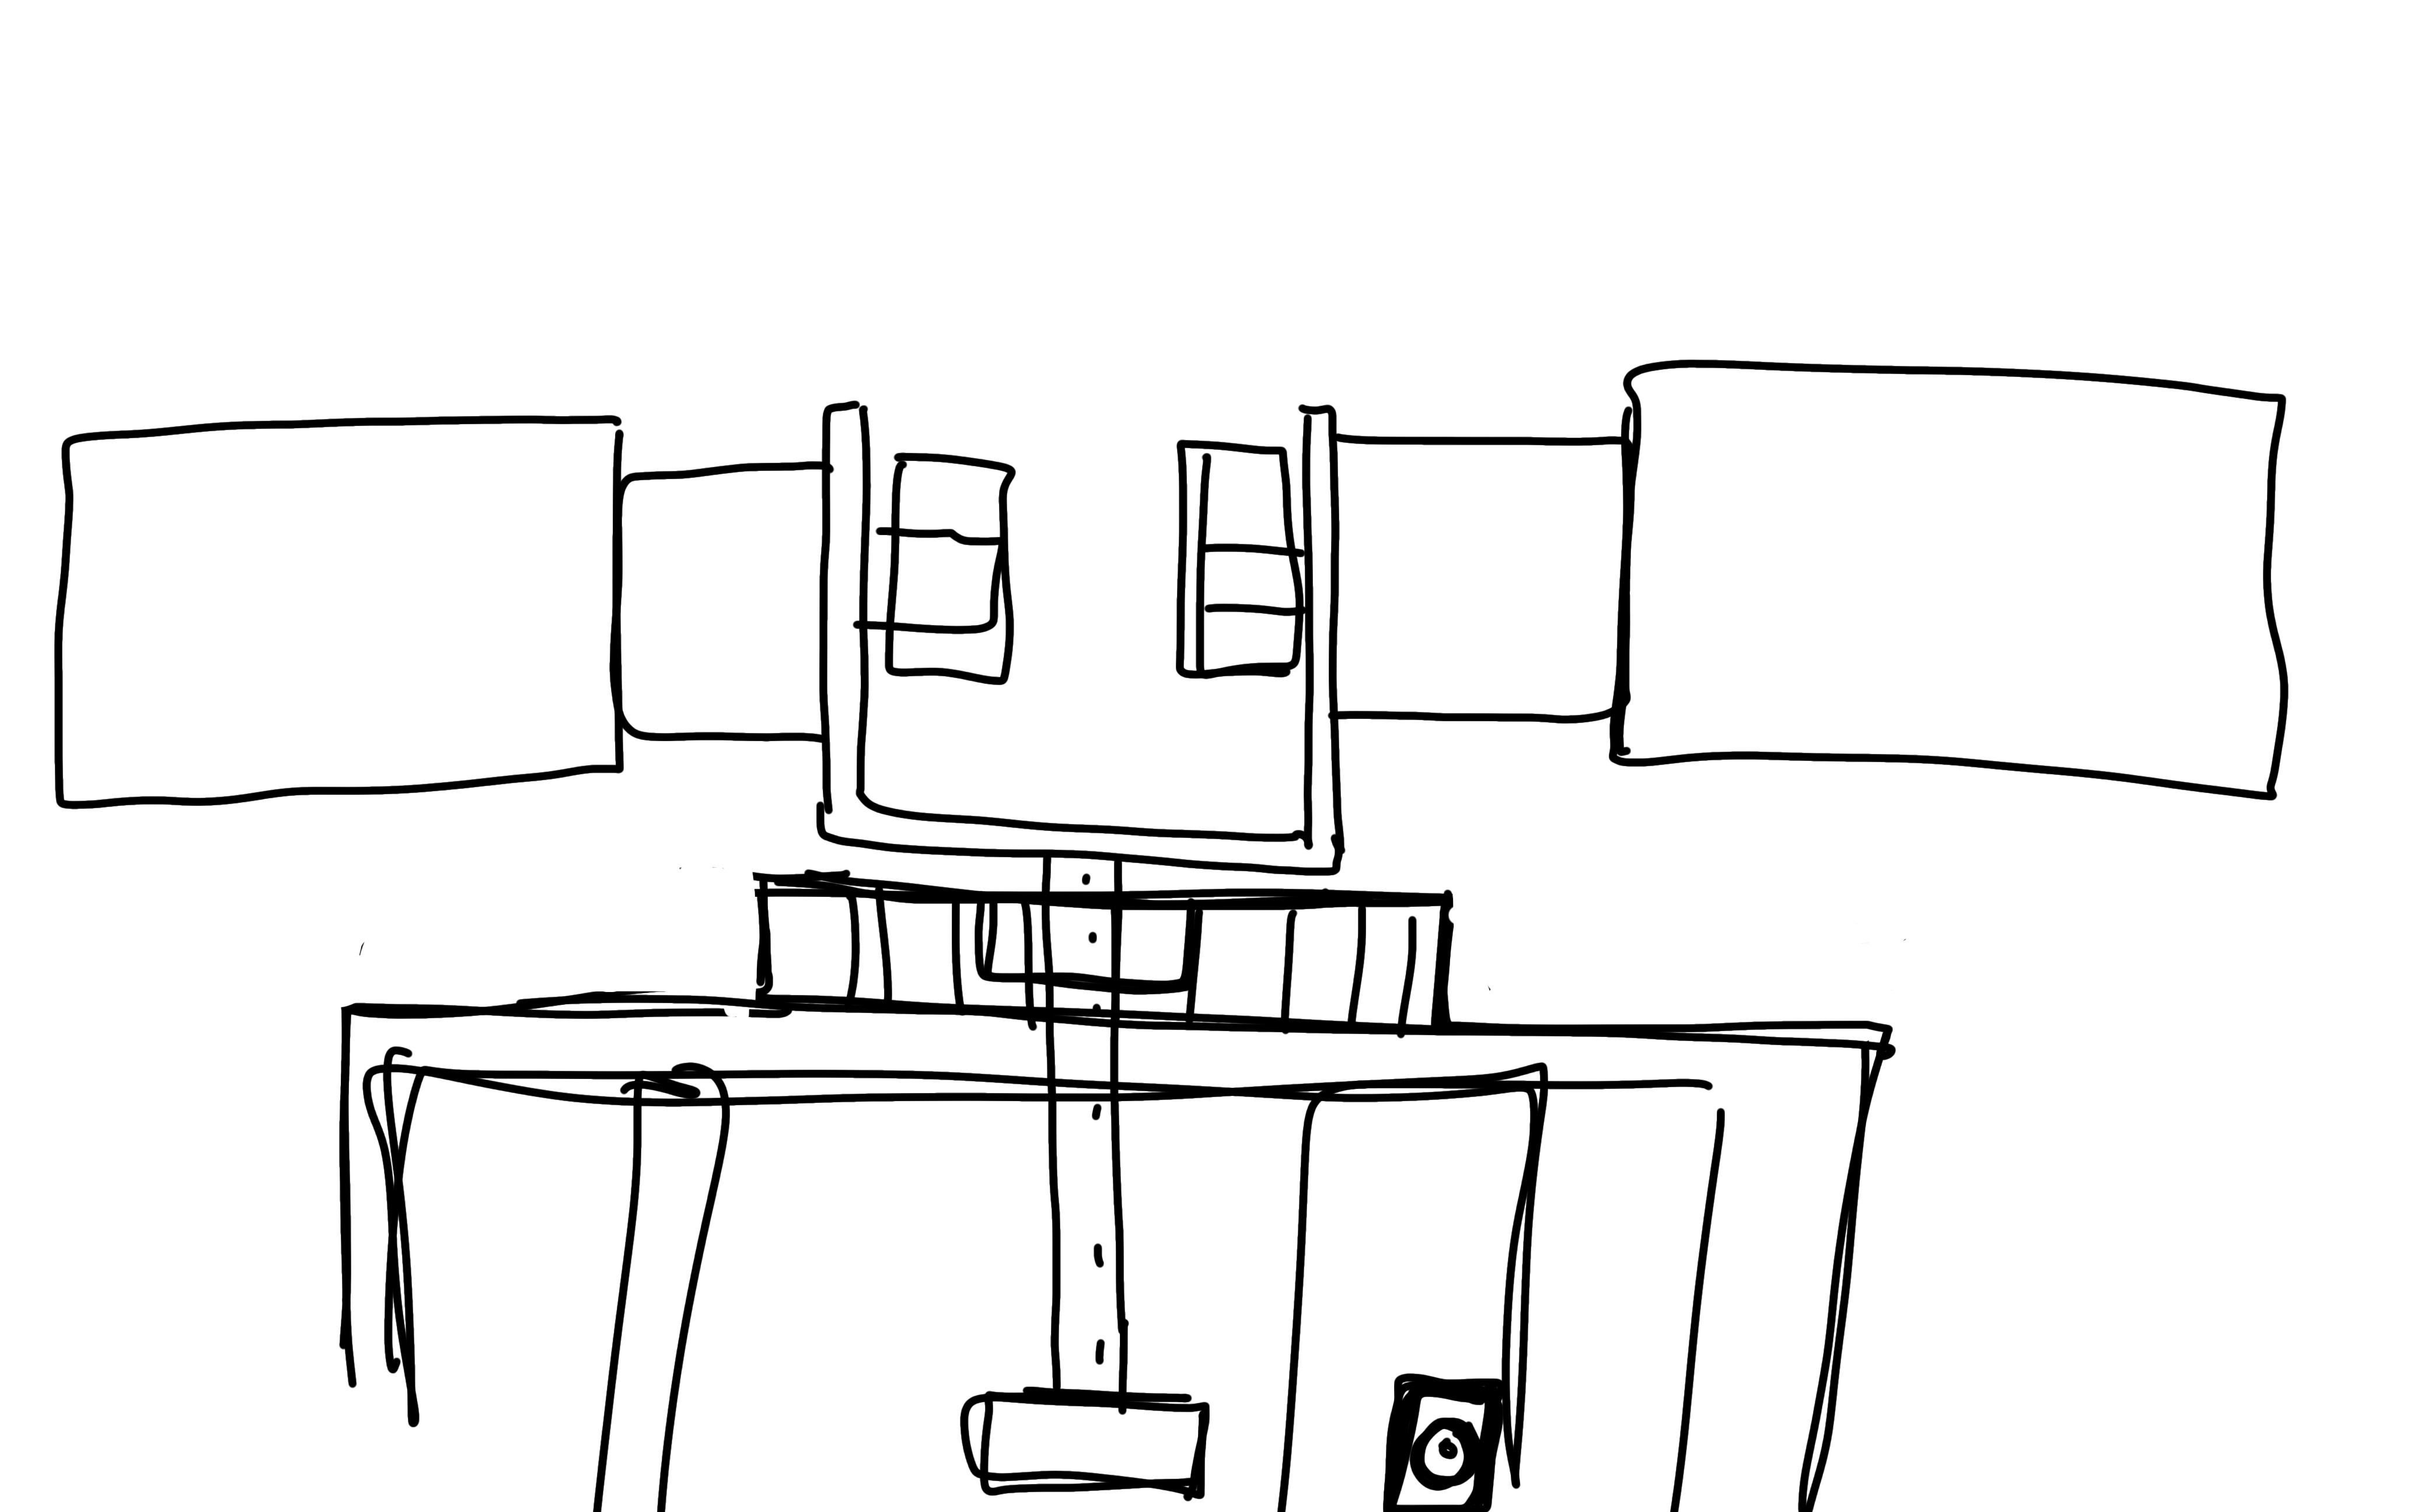
\includegraphics[width=0.4\linewidth ]{figs/boceto6.jpeg}}
  \hspace{1cm}
  \subfigure[]{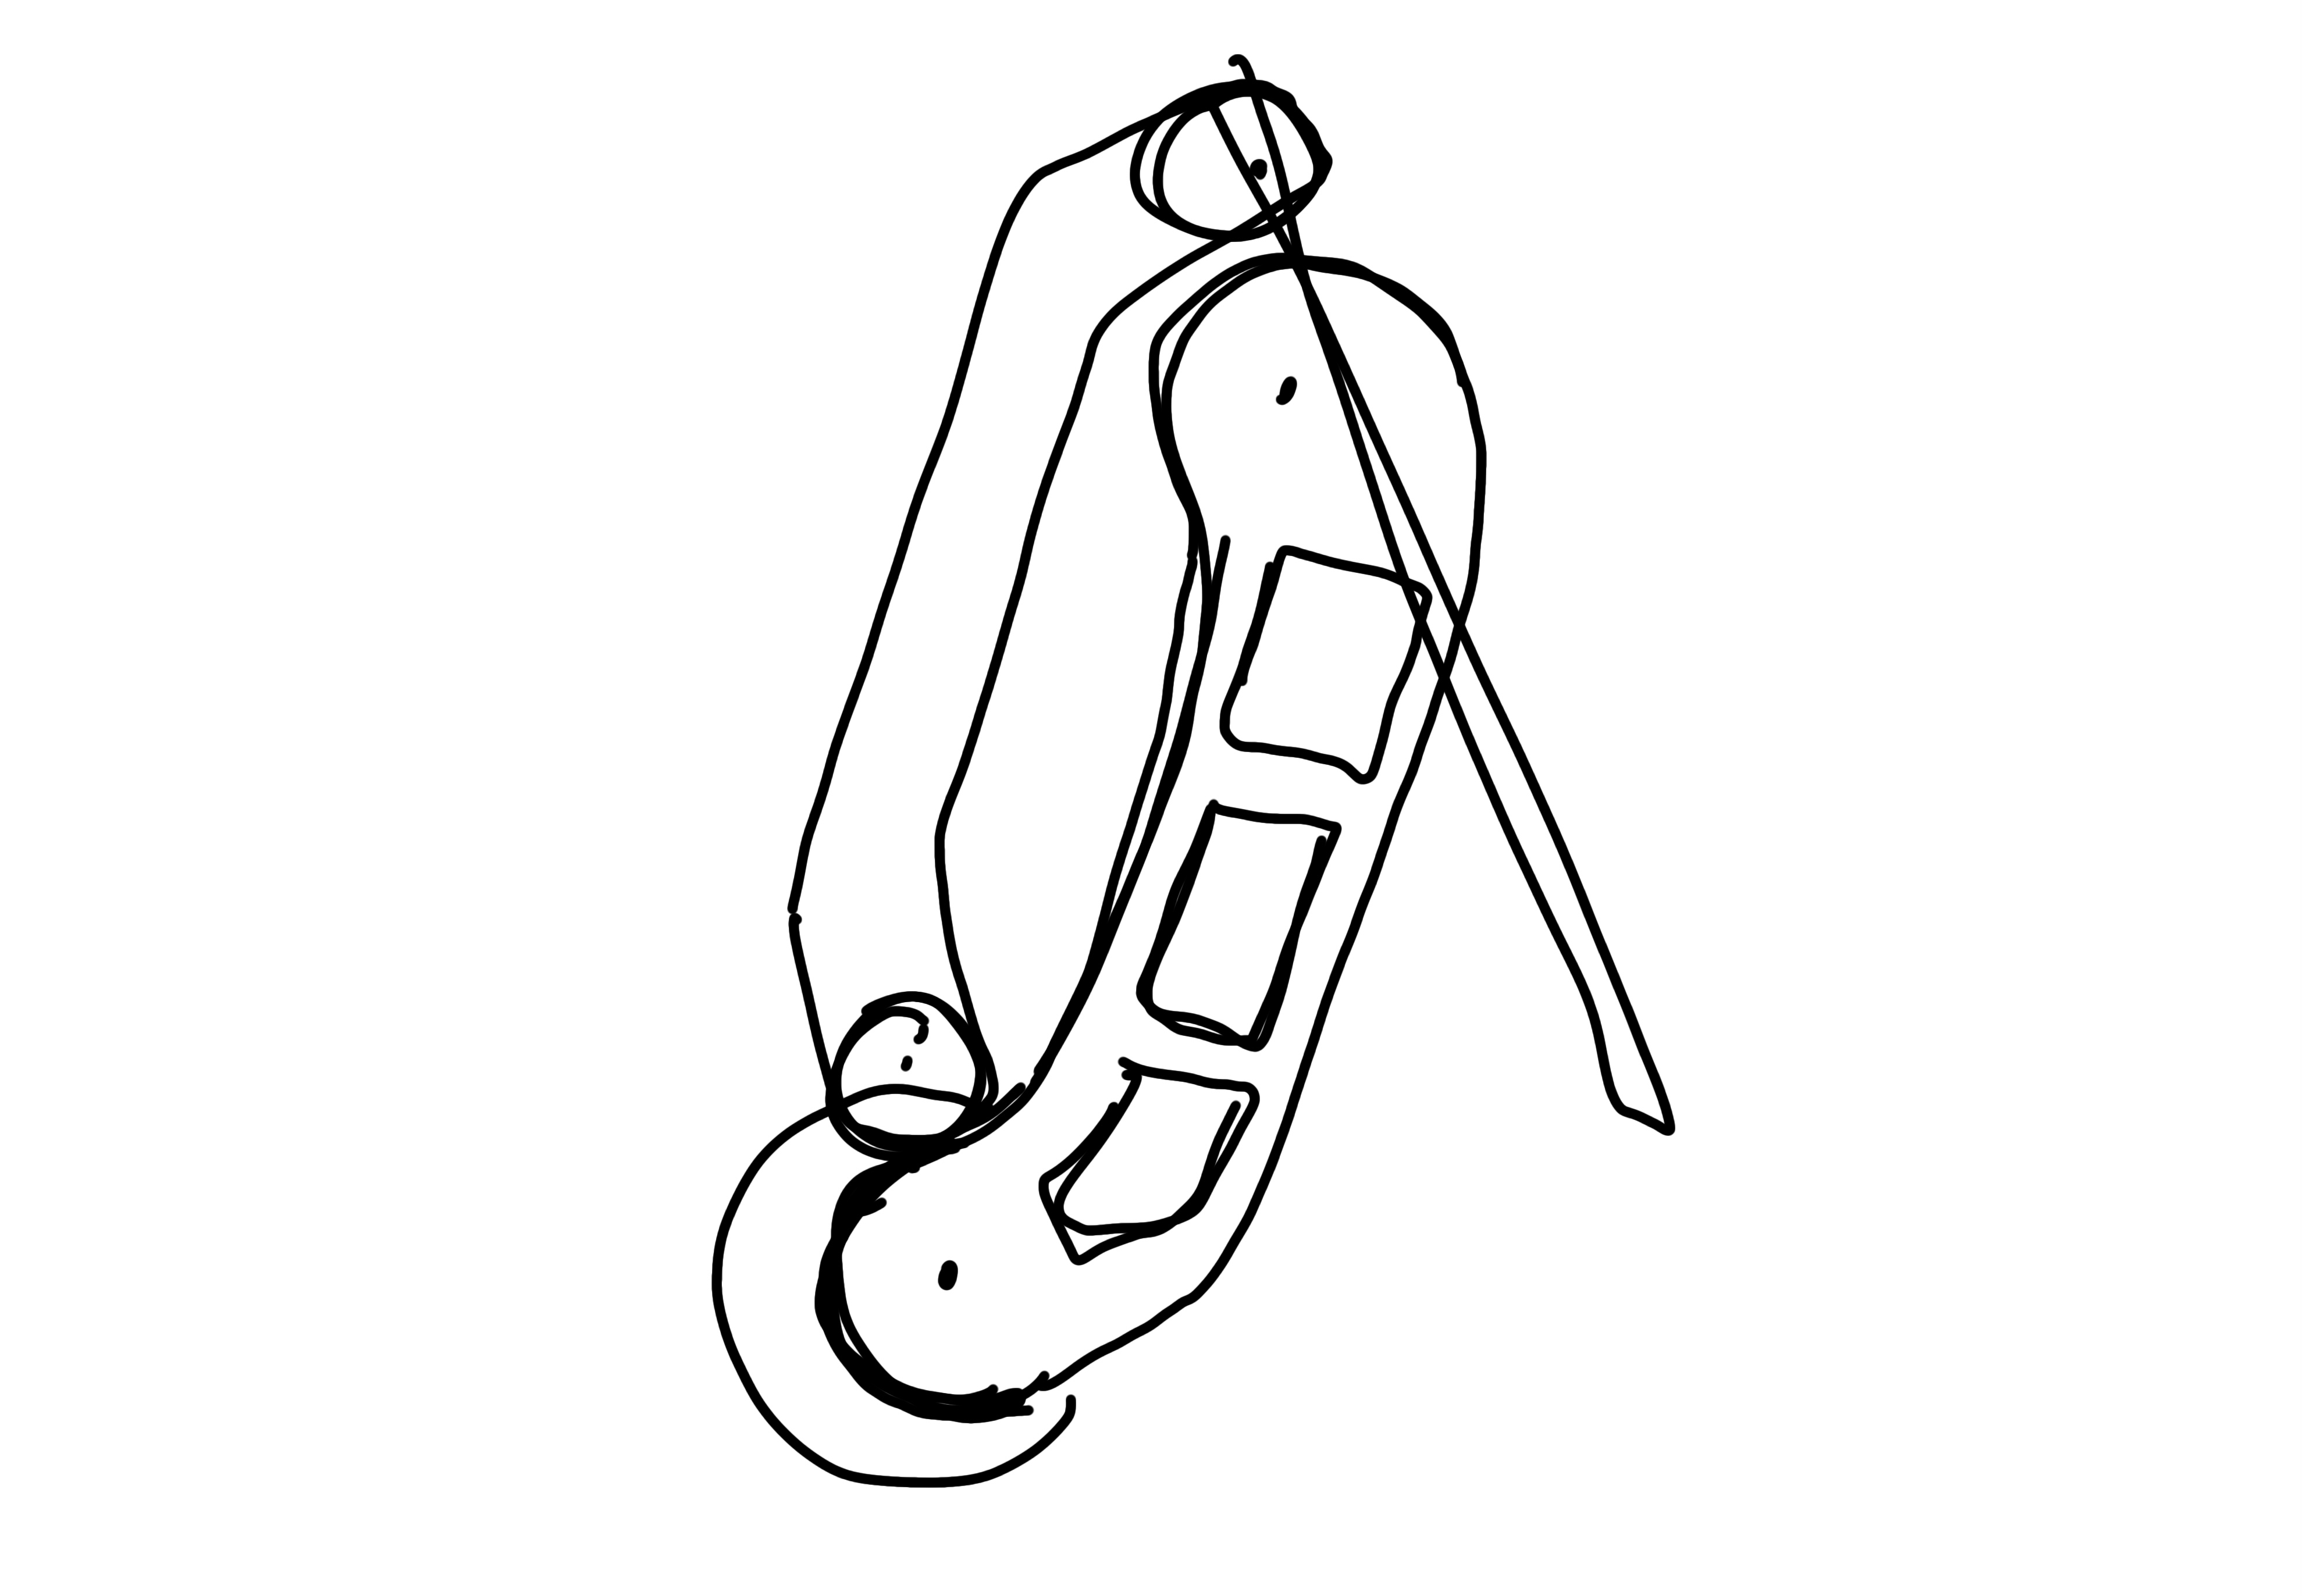
\includegraphics[width=0.4\linewidth]{figs/boceto7.jpeg}}
  \caption[Bocetos realizados]{}
  \label{fig:bocetos}
\end{figure}
\newpage
De hecho, antes pasar directamente al diseño \acs{CAD}, se realizó una versión en miniatura como prueba de concepto. 
Primeramente se hizo un boceto detallado en base al modelo alámbrico de la sección anterior. Posteriormente se llevó al 
ordenador para finalmente, imprimirlo en 3D. El proceso llevado a cabo, se puede ver en la \mbox{Figura \ref{fig:prueba_concepto}}.
\begin{figure} [h!]
  \centering    
  \subfigure[Boceto final]{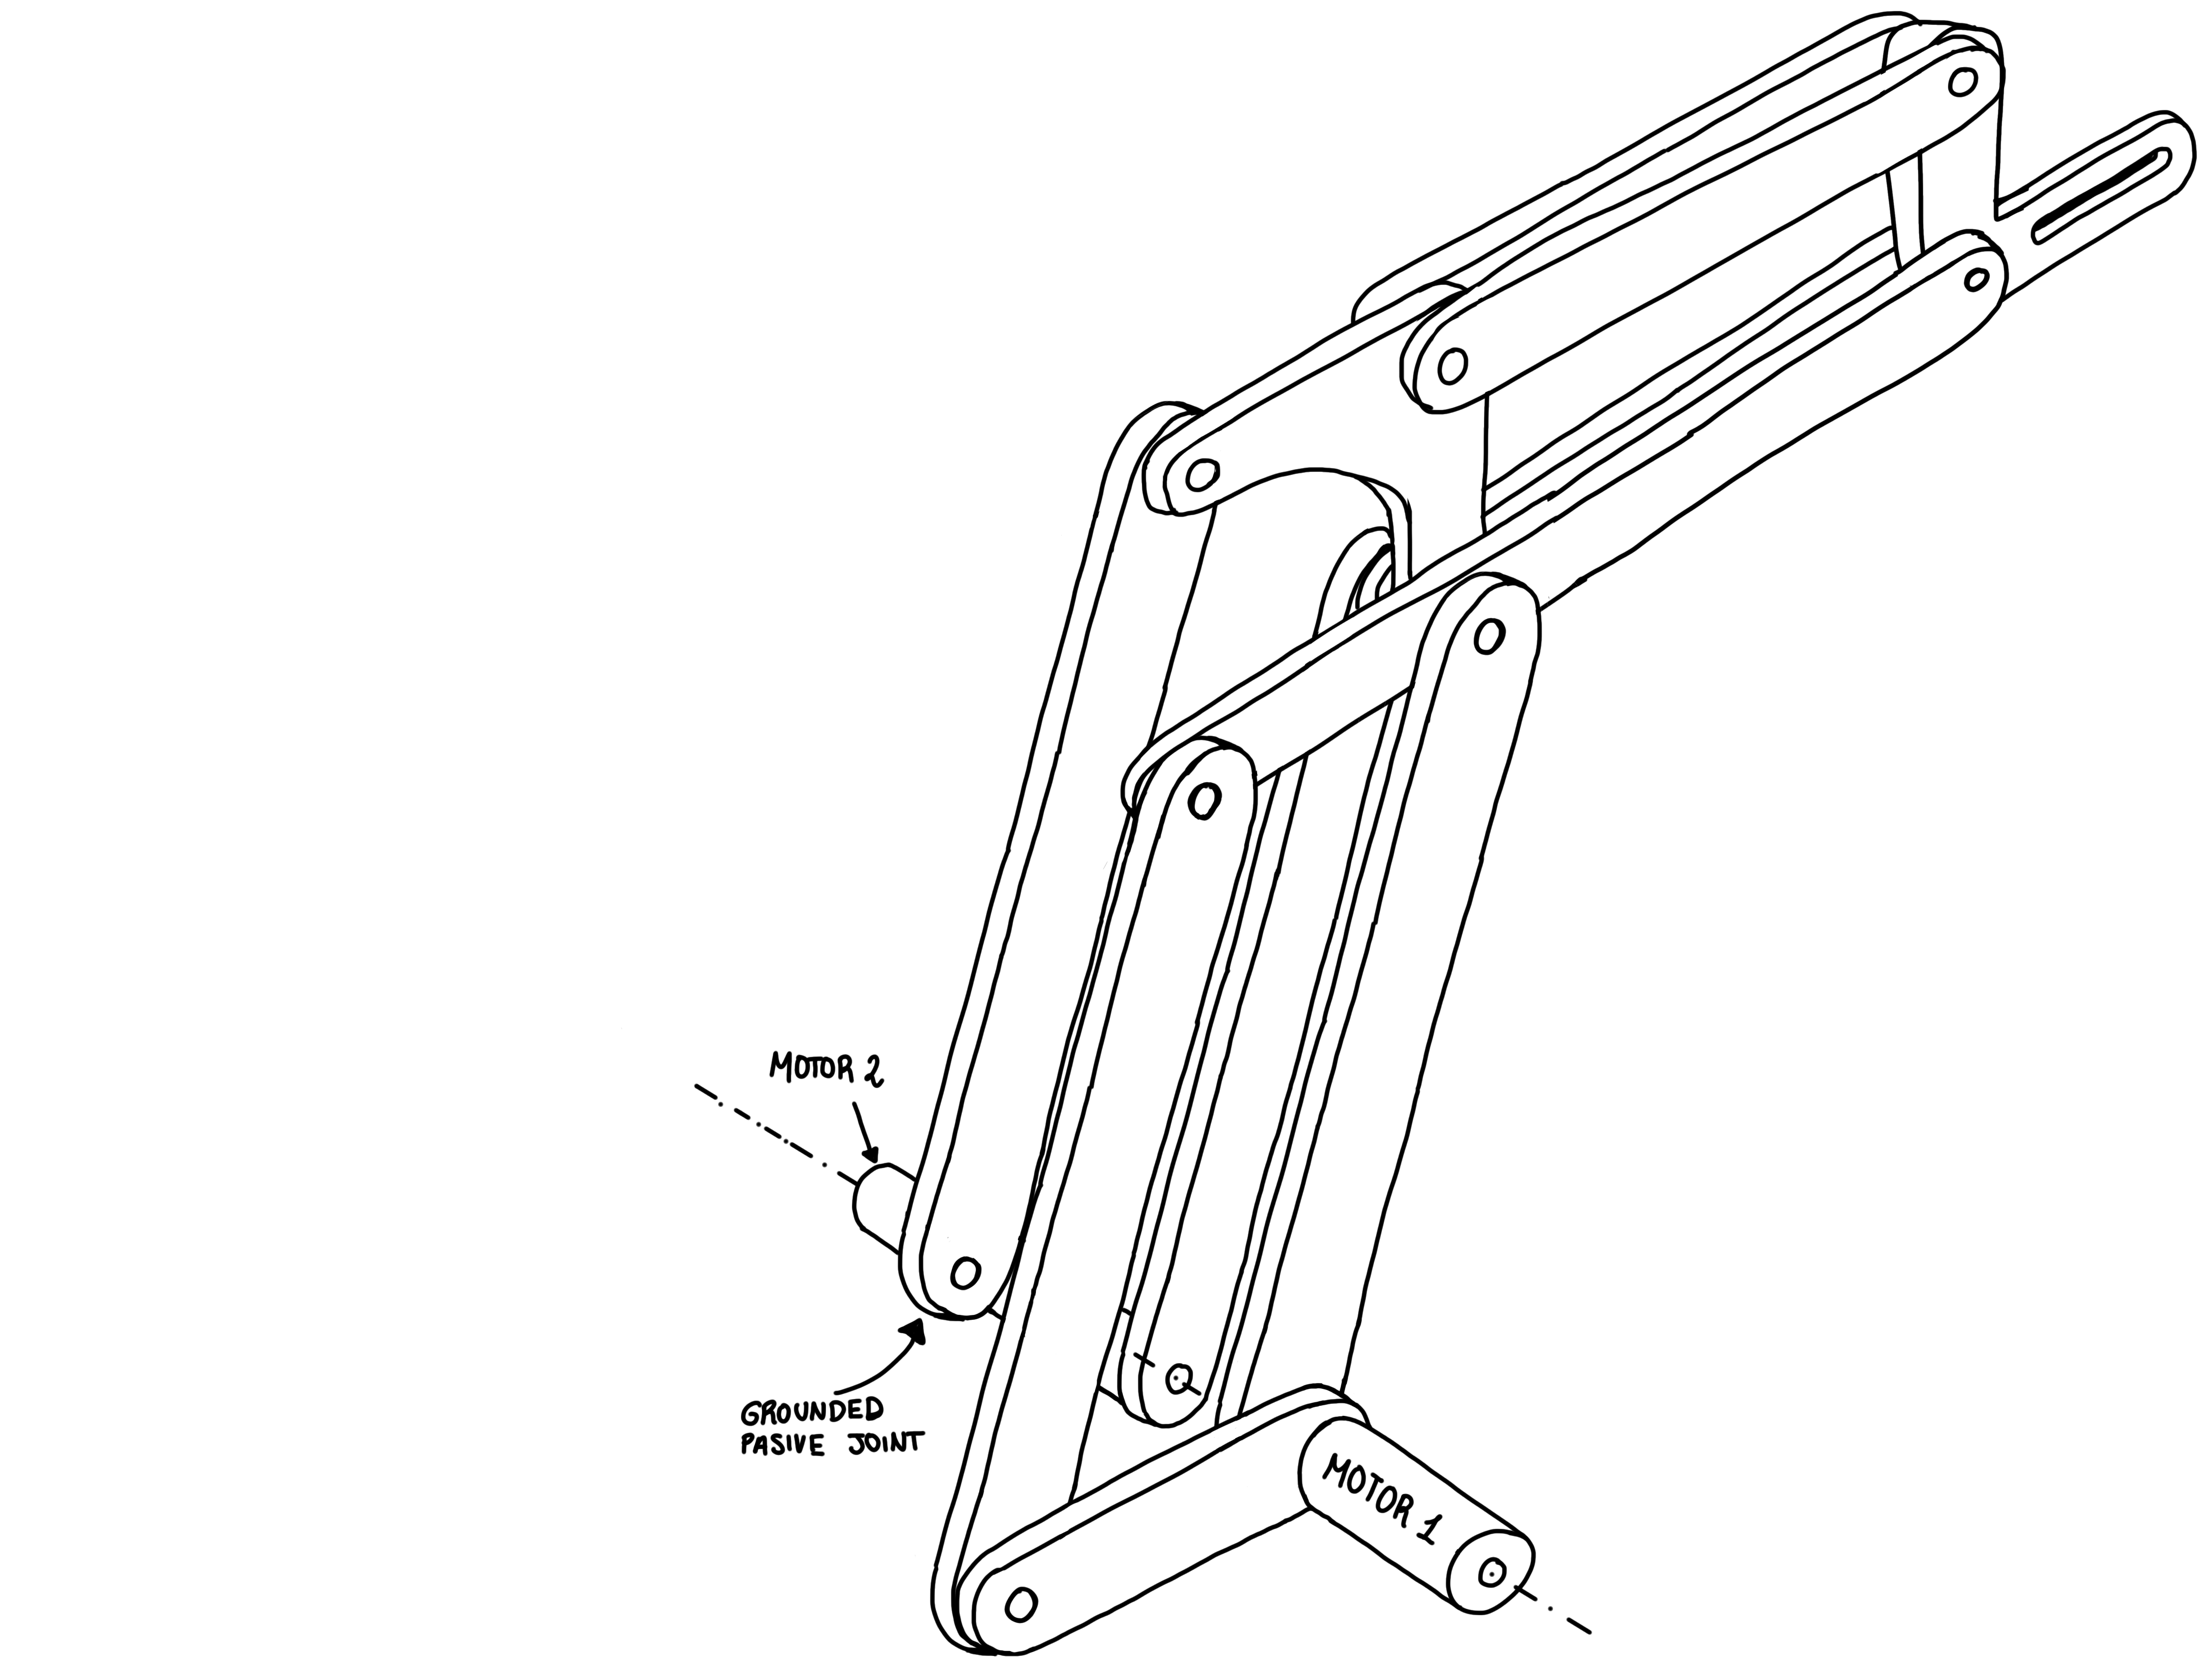
\includegraphics[width=0.35\linewidth ]{figs/boceto1.png}}
  \hspace{2.5cm}
  \subfigure[Diseño en FreeCAD]{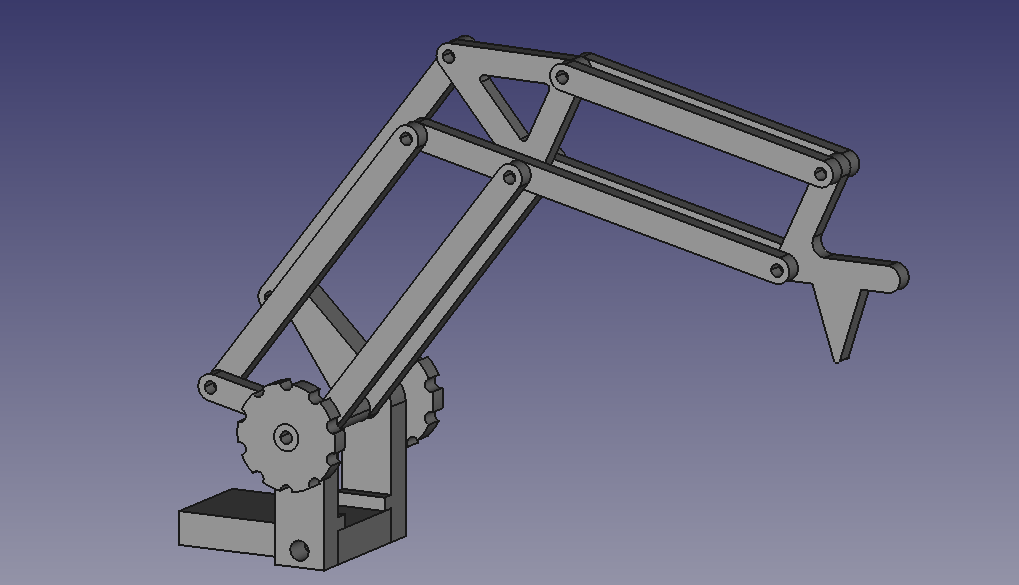
\includegraphics[width=0.45\linewidth]{figs/manipulador_prototipo.png}}
  \subfigure[Post-impresión]{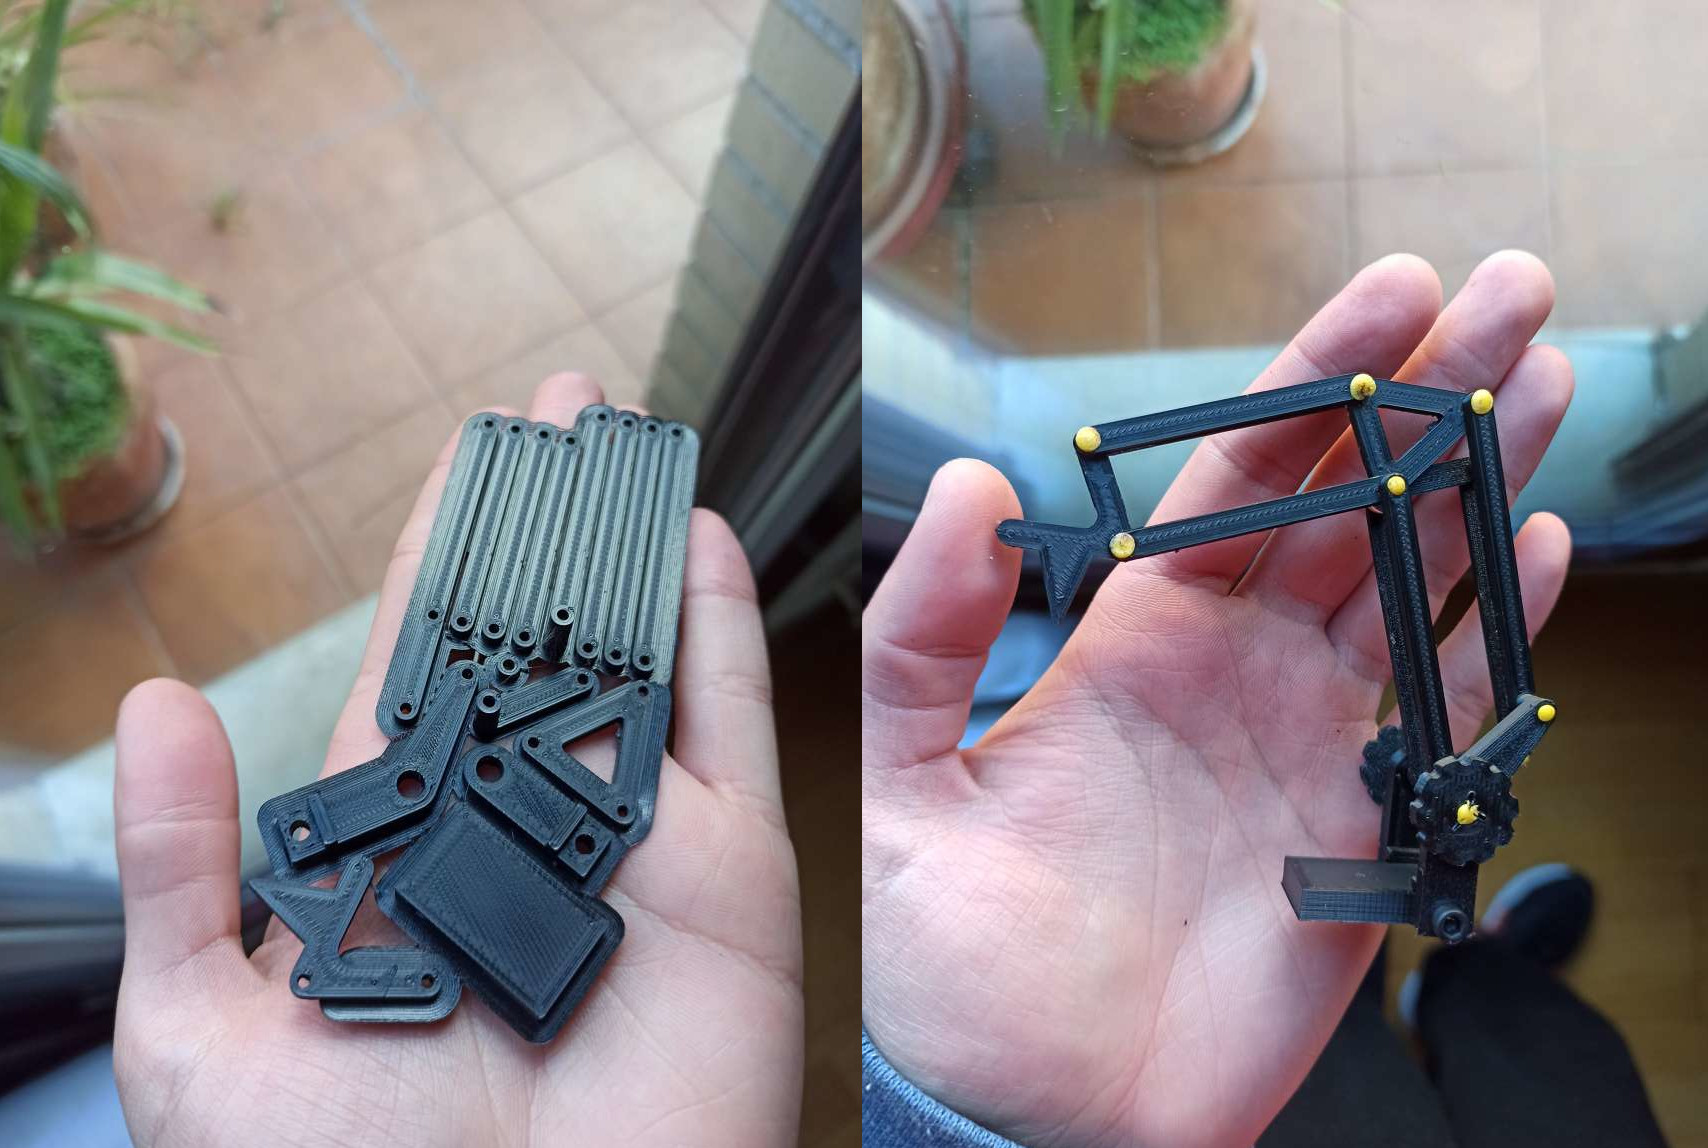
\includegraphics[width=0.45\linewidth ]{figs/prototipo_foto2.jpeg}}
  \hspace{1cm}
  \subfigure[Tamaño del prototipo]{\includegraphics[width=0.45\linewidth]{figs/prototipo_foto1.jpg}}
  \caption[Prueba de concepto]{Evolución de la prueba de concepto}
  \label{fig:prueba_concepto}
\end{figure}

El pequeño prototipo, enteramente impreso en 3D, resultó funcional y bastante resistente, por lo que se dio por bueno el 
concepto. Gracias a haber hecho esto, se pudo tener una mejor idea de la posición de cada pieza, sirviendo de gran ayuda en 
la \mbox{Sección \ref{sec:di_cad}}.
\newpage
\section{Elección de componentes electromecánicos}
\noindent En esta sección se eligen todos aquellos componentes que no pueden ser impresos en 3D y son necesarios para 
la construcción del robot. Estos componentes deben de ser asequibles y fáciles de encontrar en páginas de Internet como 
\textit{Aliexpress} o \textit{Amazon}. Con el propósito de encontrar el conjunto ideal, se 
evaluarán diversas opciones para seleccionar aquella que ofrezca las mejores prestaciones y se ajuste al presupuesto establecido.
\subsection{Motores}
\noindent El robot requiere de 3 motores que deben contar con las siguientes características:
\begin{itemize}
  \item Capacidad de entregar suficiente torque como para levantar el brazo más la carga.
  \item Se debe poder conocer su posición en cada instante.
  \item Deben poder ejercer un torque/retención estando detenidos.
\end{itemize}

Debido a esto último, no es viable usar motores convencionales con escobillas, ya que no son 
capaces de generar torque sin girar. En cambio, los motores paso a paso si son capaces de ello. Además 
suelen disponer de una gran fuerza y, aunque no estén codificados, se puede conocer su posición angular relativa debido a que avanzan en 
pequeños incrementos discretos (pasos). Como aspecto negativo, son bastante pesados. Aún así su precio no es muy elevado por lo que es 
una opción ideal para hacer un brazo robot. 

Para estimar la fuerza necesaria, se ha realizado un análisis matemático. En la Figura \ref{fig:torque} se muestra el 
escenario de mayor esfuerzo (brazo completamente extendido) y Ecuación \ref{ec:torque} tal que da como resultado 
el torque mínimo necesario para mantener esa posición.

\begin{figure} [ht!]
  \begin{center}
    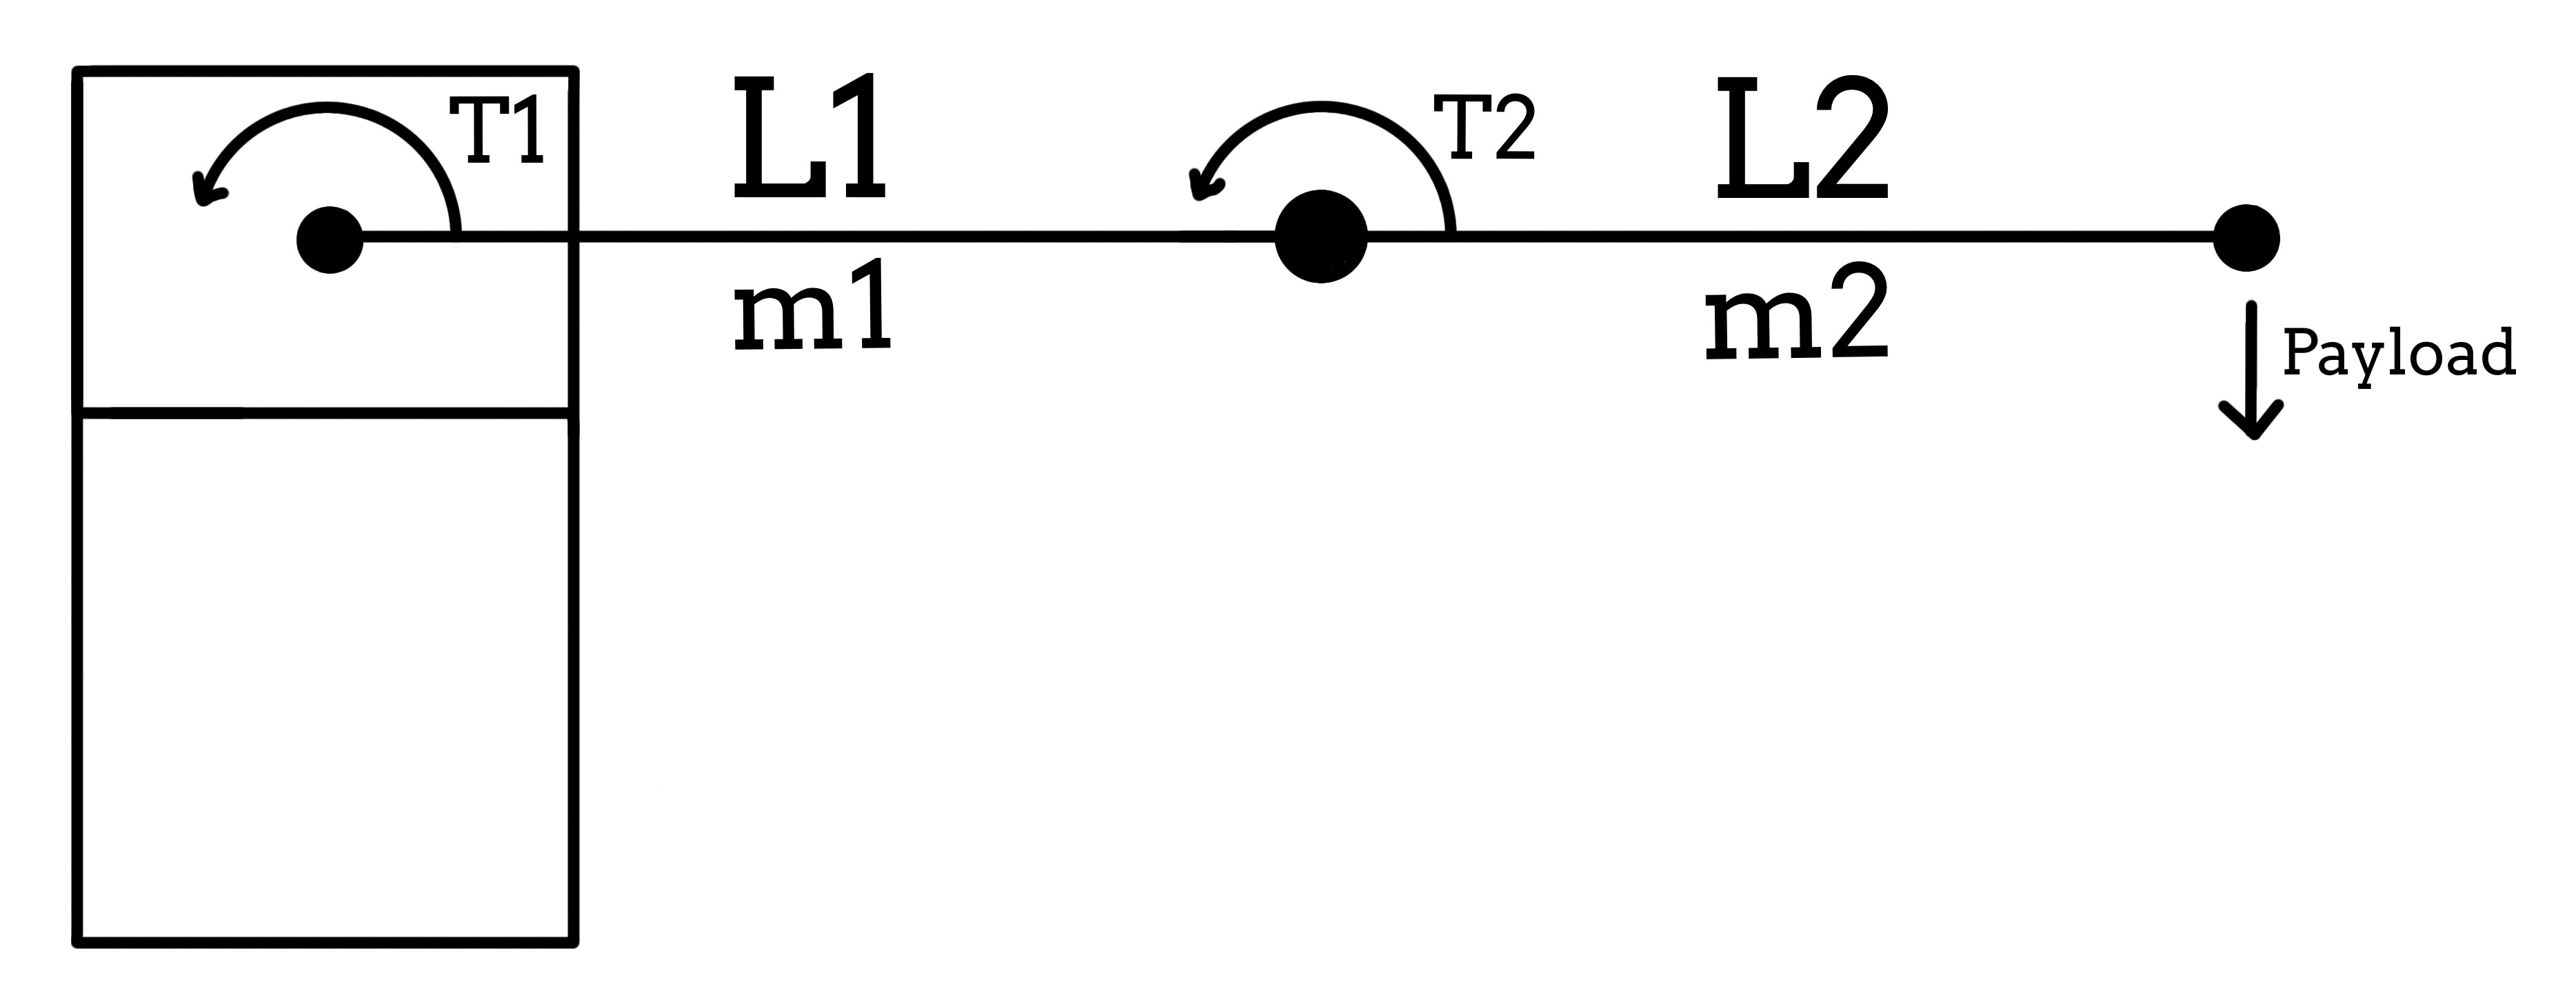
\includegraphics[width=10cm]{figs/torque.jpeg}
  \end{center}
  \caption{Dinámica del manipulador completamente extendido}
  \label{fig:torque}
\end{figure}\ 


\begin{myequation}[h!]
  \begin{equation}
    \begin{aligned}
      T1 &= m1*(L1/2) + m2*(L1 + L2/2) + payload*(L1 + L2)\\
      T2 &= m2 *(L2/2) + payload*(L1 + L2)
  \nonumber
    \end{aligned}
  \end{equation}
  \caption[Cálculo del torque necesario en la articulación más demandante]{Cálculo del torque necesario en la articulación más demandante}
  \label{ec:torque}
\end{myequation} 
Teniendo en cuenta que cada eslabón mide 17cm y se desea levantar una carga máxima de 300g, el valor de 
torque necesario en la primera articulación es y tal en la segunda.

Los motores paso a paso se dividen en diferentes categorías según su potencia y rendimiento. En este caso, se empleará 
un motor perteneciente a la categoría Nema, específicamente el Nema 17. Esta elección se basa en su amplia disponibilidad, facilidad 
para adquirirlos y su precio razonable.

Dentro de la categoría Nema 17, todos los motores comparten el mismo factor de forma, diferenciándose únicamente en su longitud, lo que 
afecta directamente al torque que pueden proporcionar. A mayor longitud, mayor capacidad de ejercer torque. Debido a esto, se ha optado 
por utilizar los más largos posibles dentro del presupuesto. Concretamente, 3 Nema 17 de 60mm (0.6 N.m) con un coste total de 55\euro. 

Aunque el motor Nema 17 no es suficiente para suministrar por sí solo el torque necesario, se tiene previsto utilizar una reductora más 
adelante para multiplicar la fuerza final de la articulación. Esta estrategia evita la necesidad de utilizar un motor más grande y 
costoso. La reductora aumentará cinco veces el torque disponible para la articulación, permitiendo así un rendimiento adecuado 
sin comprometer la elección del motor Nema 17.

\begin{figure} [ht!]
  \begin{center}
    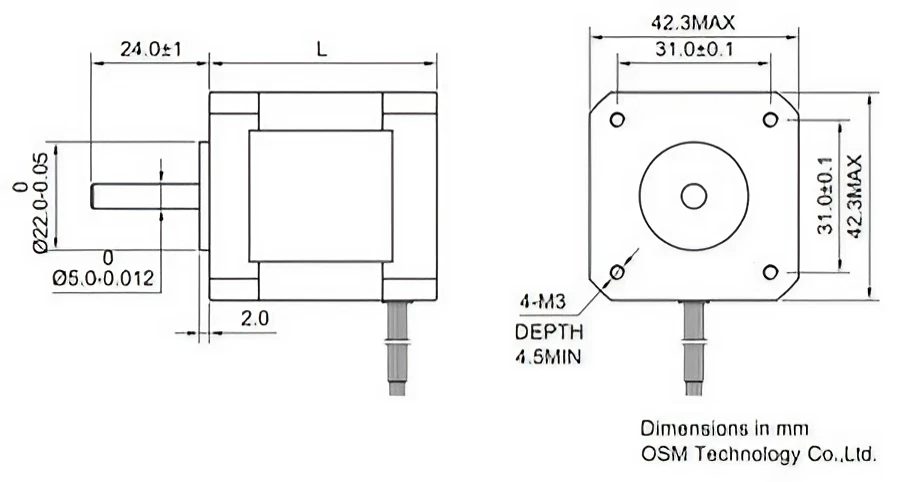
\includegraphics[width=11cm]{figs/MotorsNema.png}
  \end{center}
  \caption{Dimensiones de los motores Nema17 \footnote{\url{https://reprap.org/wiki/NEMA_17_Stepper_motor}}}
  \label{fig:nema}
\end{figure}\ 

\subsection{Reductora}
\noindent Para reducir la velocidad de giro de un motor y convertirla en fuerza, se requiere implementar una 
reductora. Existen varias opciones para lograrlo, como el uso de engranajes (normales, planetarios, helicoidales, etc.) 
o correas (lisas y dentadas).

En este caso, se ha optado por utilizar correas dentadas en lugar de engranajes debido a que los engranajes 
tienden a introducir holguras en el movimiento final, ocasionando imprecisión e incertidumbre en los movimientos 
del robot. Por el contrario, las correas dentadas utilizan tensores para mantener siempre el contacto con 
ambas poleas, lo que resulta en un movimiento más preciso y confiable.

Se ha elegido el tipo de correa GT2 (Figura \ref{fig:correa}), ampliamente utilizado en impresoras 3D, por su bajo coste y fácil 
disponibilidad en el mercado. Dentro de esta categoría, se ha seleccionado un ancho de 6 mm, el más 
económico y adecuado para la aplicación requerida. El largo de cada correa se concretará en la \mbox{Sección \ref{sec:di_cad}}.
\begin{figure} [ht!]
  \begin{center}
    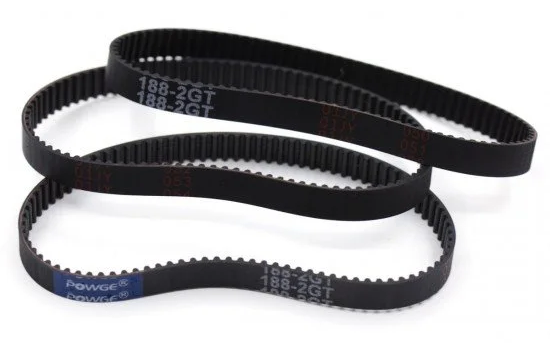
\includegraphics[width=8cm]{figs/correa.png}
  \end{center}
  \caption{Ejemplo de correa GT2}
  \label{fig:correa}
\end{figure}\ 

Además, las poleas necesarias para este tipo de correas se pueden diseñar e imprimir en 3D de manera 
sencilla y económica. Esto permite personalizar el número de dientes de las poleas según las 
necesidades del robot, con un costo prácticamente nulo.

Para dos de los tres grados de libertad del robot, se ha elegido utilizar una combinación de poleas: una polea comercial de 
metal con 20 dientes unida al eje del motor y otra polea impresa en 3D con 100 dientes, logrando una reducción de 1:5\footnote{
  La reducción 1:5 indica que, por cada vuelta del motor, el sistema de transmisión proporciona aproximadamente 1/5 de vuelta en el eje de salida.
}. En el 
tercer grado de libertad, se pretende emplear una polea con 120 dientes \mbox{(reducción 1:6)} siguiendo el mismo principio.

\subsection{Controladores}
\noindent En el mundo del \textit{maker}, existe un factor de forma común para controladores de motores paso a paso de baja corriente (hasta 2A). Debido a esto, 
la mayoría de los controladores disponibles en el mercado son intercambiables entre sí, aunque varían en la tecnología interna y en sus 
capacidades técnicas.

En el mercado actual, se pueden encontrar diversos controladores diseñados específicamente para motores paso a paso bipolares. Estos 
controladores se diferencian en términos de tecnología y características técnicas que ofrecen. Algunos de los controladores más comunes 
y populares son basados en chips como el A4988, DRV8825 o TMC2208, entre otros. Concretamente, se han seleccionado cuatro de ellos, cuyas 
especificaciones pueden verse en el Cuadro \ref{cuad:controladores}.
\begin{table}[htbp]
  \centering
  \caption{Comparación de especificaciones de los controladores existentes}
  \label{cuad:controladores}
  \begin{tabular}{|c|c|c|c|c|c|}
      \hline
      \multirow{2}{*}{Modelo} & Voltaje de & Corriente & \multirow{2}{*}{Microstepping} & Nivel de & \multirow{2}{*}{Precio} \\
                             & alimentación & máxima & & ruido &\\
      \hline
      A4988 & 8-35V & 2A & Hasta 1/16 & Muy ruidoso & 1\euro \\
      \hline
      DRV8825 & 8.2-45V & 2.5A & Hasta 1/32 & Ruido aceptable & 2\euro \\
      \hline
      TMC2225 & 4.7-36V & 2A & Hasta 1/32 & Bajo ruido  & 2.8\euro \\
      \hline
      TMC2209 & 5.5-28V & 2.5A & Hasta 1/256 & Totalmente silencioso & 3.4\euro \\
      \hline
  \end{tabular}
\end{table}
\begin{figure} [h!]
  \centering    
  \subfigure[A4988]{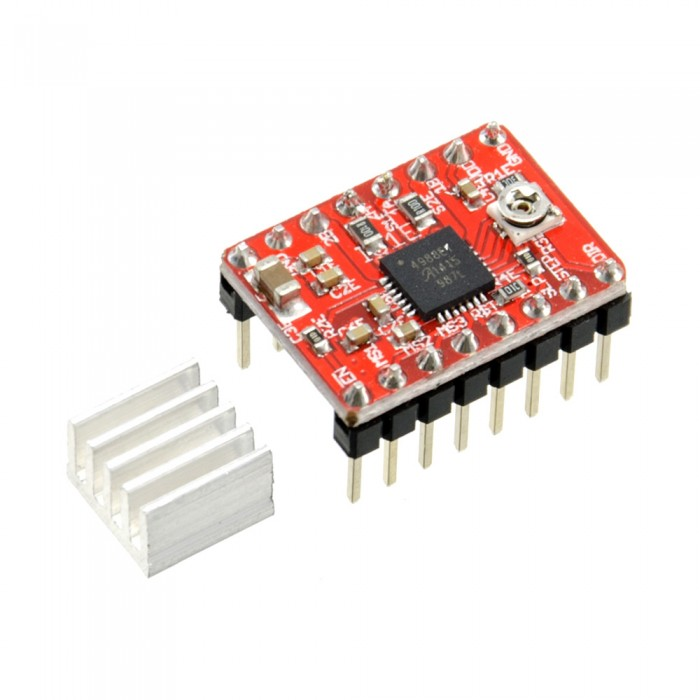
\includegraphics[width=0.2\linewidth ]{figs/a4988.jpg}}
  \hspace{0.5cm}
  \subfigure[DRV8825]{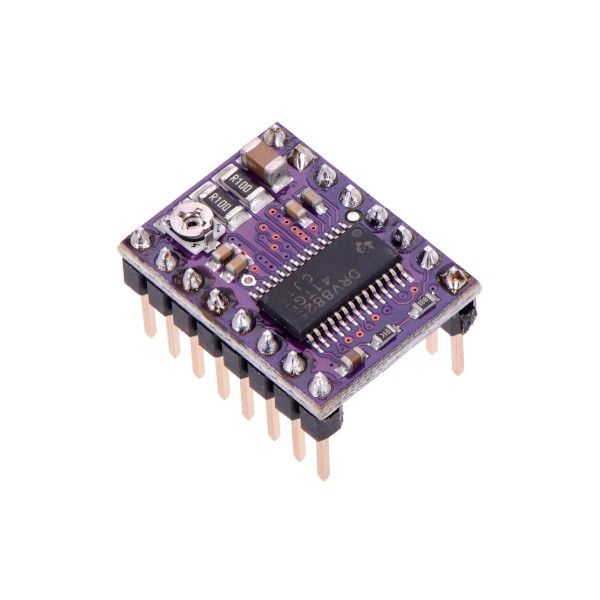
\includegraphics[width=0.2\linewidth]{figs/drv8825.jpg}}
  \hspace{0.5cm}
  \subfigure[TMC2225]{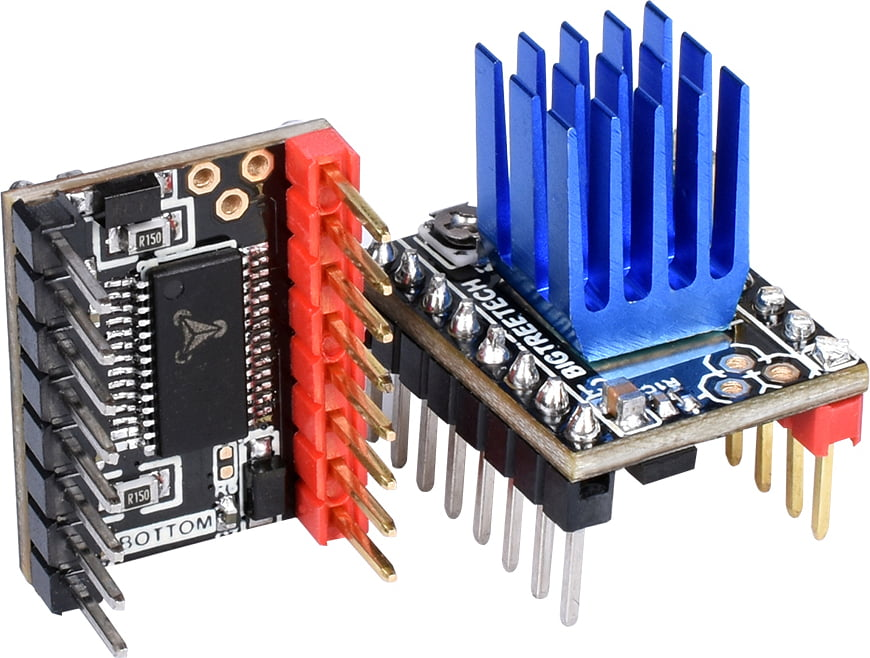
\includegraphics[width=0.2\linewidth]{figs/tmc2225.jpg}}
  \hspace{0.5cm}
  \subfigure[TMC2209]{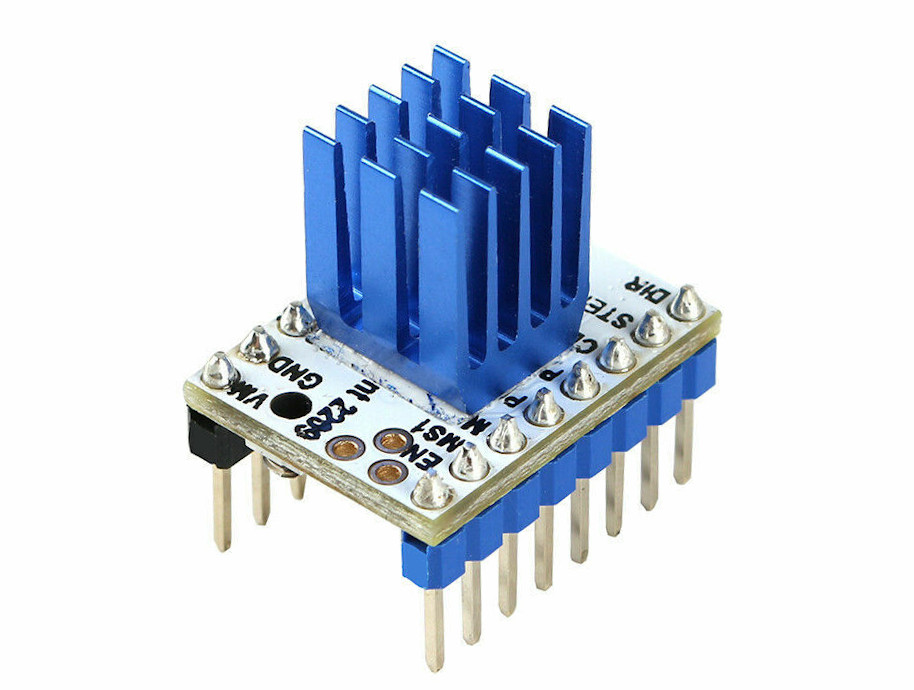
\includegraphics[width=0.2\linewidth]{figs/TMC2209.jpg}}
  \caption[Controladores existentes en el mercado]{Aspecto de los controladores}
  \label{fig:controladores}
\end{figure}

Debido a que se pretende utilizar motores Nema 17 de más de 2A, la decisión debe estar entre el DRV8825 y el TMC2209. Finalmente, se 
ha elegido este último debido a que es realmente silencioso e incorpora una tecnología superior que garantiza una señal más definida que 
evita la pérdida de pasos del motor. Además, a la hora de adquirirlo, suele venir acompañado de un disipador de calor más grande que, unido 
a su mayor eficiencia energética, se traduce en una menor cantidad de calor dentro de nuestro robot. 

\subsection{Placa base CNC}
\noindent La placa base es una tarjeta de circuito impreso que proporciona conexiones físicas y eléctricas entre los diferentes componentes y 
unifica estos en un mismo componente. 

En el caso de aquellas utilizadas en el mundo de las CNCs, tienen la posibilidad de montar controladores paso a paso y, o bien 
integran un microcontrolador en la propia placa, o bien tienen la posibilidad de acloparse a uno concreto
(\textit{shields}\footnote{(placa adicional que se acopla a otras para aumentar su funcionalidad y características)}).  



En el mercado existen cantidad de ellas, entre las que destacan principalmente dos: Arduino CNC Shield V3 y MKS DLC32 (Figura \ref{fig:placas_candidatas})
\begin{figure} [h!]
  \centering    
  \subfigure[Arduino Uno CNC Shield]{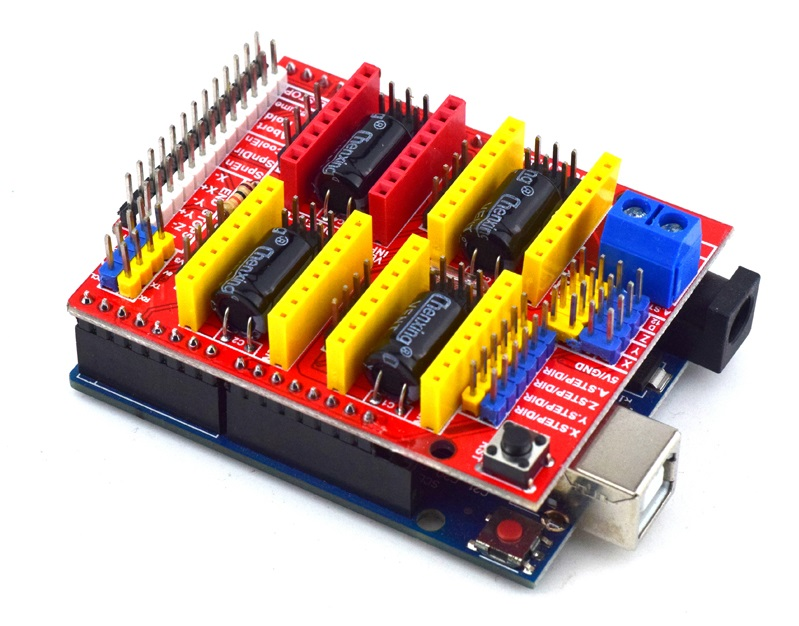
\includegraphics[width=0.4\linewidth ]{figs/uno_shield.jpg}}
  \hspace{0.5cm}
  \subfigure[MKS DLC32]{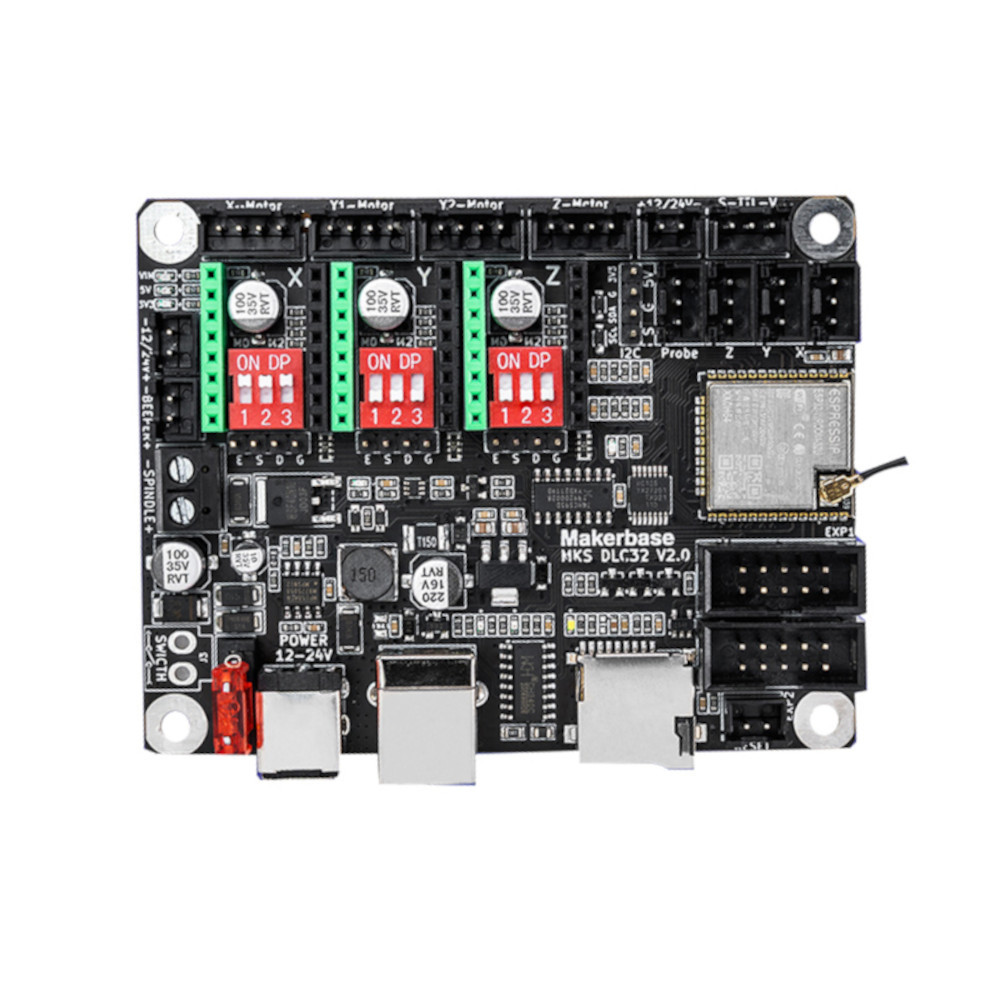
\includegraphics[width=0.4\linewidth]{figs/mksdlc32.jpg}}
  \caption[Placas base candidatas]{Placas base candidatas}
  \label{fig:placas_candidatas}
\end{figure}
 
Finalmente se ha optado por la segunda ya que la diferencia entre ambas es de a penas 6 euros y en cambio, es muy superior en características. Esta placa 
incorpora un microcontrolador ESP32 mucho más avanzado y rápido que el AtMega328p usado en el Arduino Uno. Además incorpora un transistor MOSFET de 
gran potencia que permite controlar una salida de hasta 24v mediante PWM\footnote{
PWM (Pulse Width Modulation) es una técnica de control que varía el ancho de un pulso eléctrico para regular la potencia entregada a un dispositivo o 
componente, como motores o luces, permitiendo controlar su velocidad o intensidad de manera eficiente.}. Por lo general, es una placa mejor acabada, 
con un hardware más moderno y está pensada para que su montaje eléctrico no de lugar a error.

\newpage
\subsection{Fuente de alimentación}
\noindent Es el elemento encargado de suministrar la energía a todo el sistema eléctrico del robot. La elección de este componente viene dada 
por las características y necesidades de los componentes elegidos anteriormente. 

Para conocer esto, se debe realizar una estimación del consumo en base a las especificaciones que ofrecen los fabricantes. En base a esto, la mayor 
parte del consumo viene dado por los propios motores que se encontrarán permanentemente excitados para no desplomar el robot. Concretamente,
cada uno consume en torno a 7W, haciendo un total de 21W. A esto hay que añadirle el consumo del microcontrolador y la potencia 
perdida en forma de calor en los controladores (unos 4W). Sumado a ello, se deben tener en cuenta los 3W consumidos por el electroimán. Finalmente, 
el consumo estimado ronda los 35W.

En base a la estimación, se debe encontrar una fuente de alimentación que sea capaz de dar, al menos, esa potencia de manera continuada. En cuanto al 
voltaje, cualquiera en el rango de 12 a 24v es válido. Se recomienda utilizar una del mayor voltaje posible ya que, en teoría, es más eficiente 
debido a que la corriente que debe entregar es menor, además de lidiar mejor con las caídas de tensión en movimientos rápidos.

Dicho esto, es posible también alimentar el robot mediante un cargador típico de 19v de un portátil. Aún así, la fuente adquirida para 
este proyecto es de 24V 150W para poder realizar todas las mediciones de consumos de la Sección \ref{sec:consumo}, descartando a la fuente 
como factor limitante. Aún así, el precio de esta fuente es de solo 15\euro.

\subsection{Rodamientos}
\label{sec:bridas}
\noindent Para mejorar la eficiencia de las articulaciones y garantizar que todas roten con suavidad, se pretende hacer uso de rodamientos 
en cada una de ellas. 
Existen diferentes tipos de rodamientos en el mercado pero se ha optado por un tipo de rodamiento concreto para este proyecto. 
Se pretenden utilzar rodamientos brida como el de la Figura \ref{fig:rodamientos_fushi}. La razón principal de su uso es su peculiar forma. Este tipo 
de rodamiento tiene un borde en el extremo que hace de borde que lo hace ideal para insertar en piezas 3D y garantizar 
que nunca se puedan salir de su sitio mientras exista un tornillo que lo fije (Véase la Figura \ref{fig:ejemplo_rodamiento}).

\begin{figure} [ht!]
  \centering  
  \subfigure[Rodamientos F695-2RS Fushi \footnote{\url{https://es.aliexpress.com/item/32850989216.html}}]{\label{fig:rodamientos_fushi}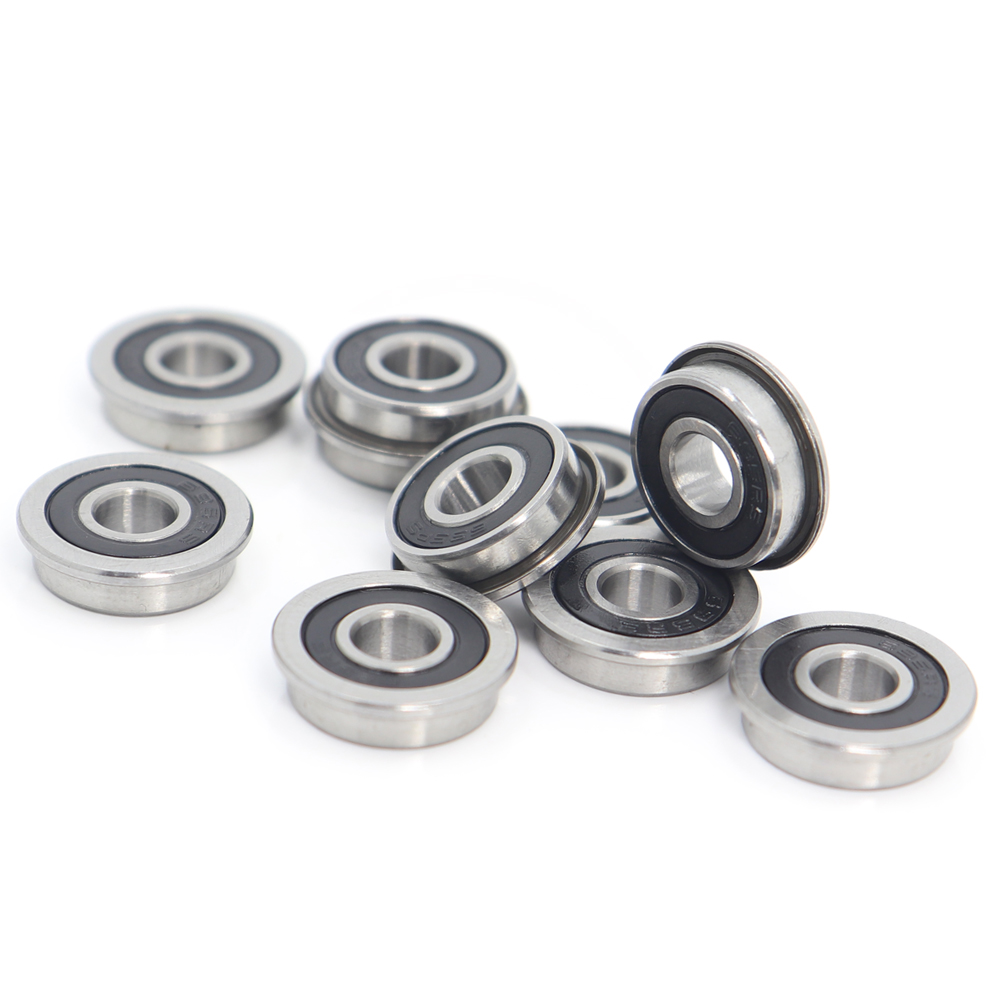
\includegraphics[width=0.4\linewidth ]{figs/F695-2RS.jpeg}}
  \hspace{0.5cm}
  \subfigure[Ejemplo de uso]{\label{fig:ejemplo_rodamiento}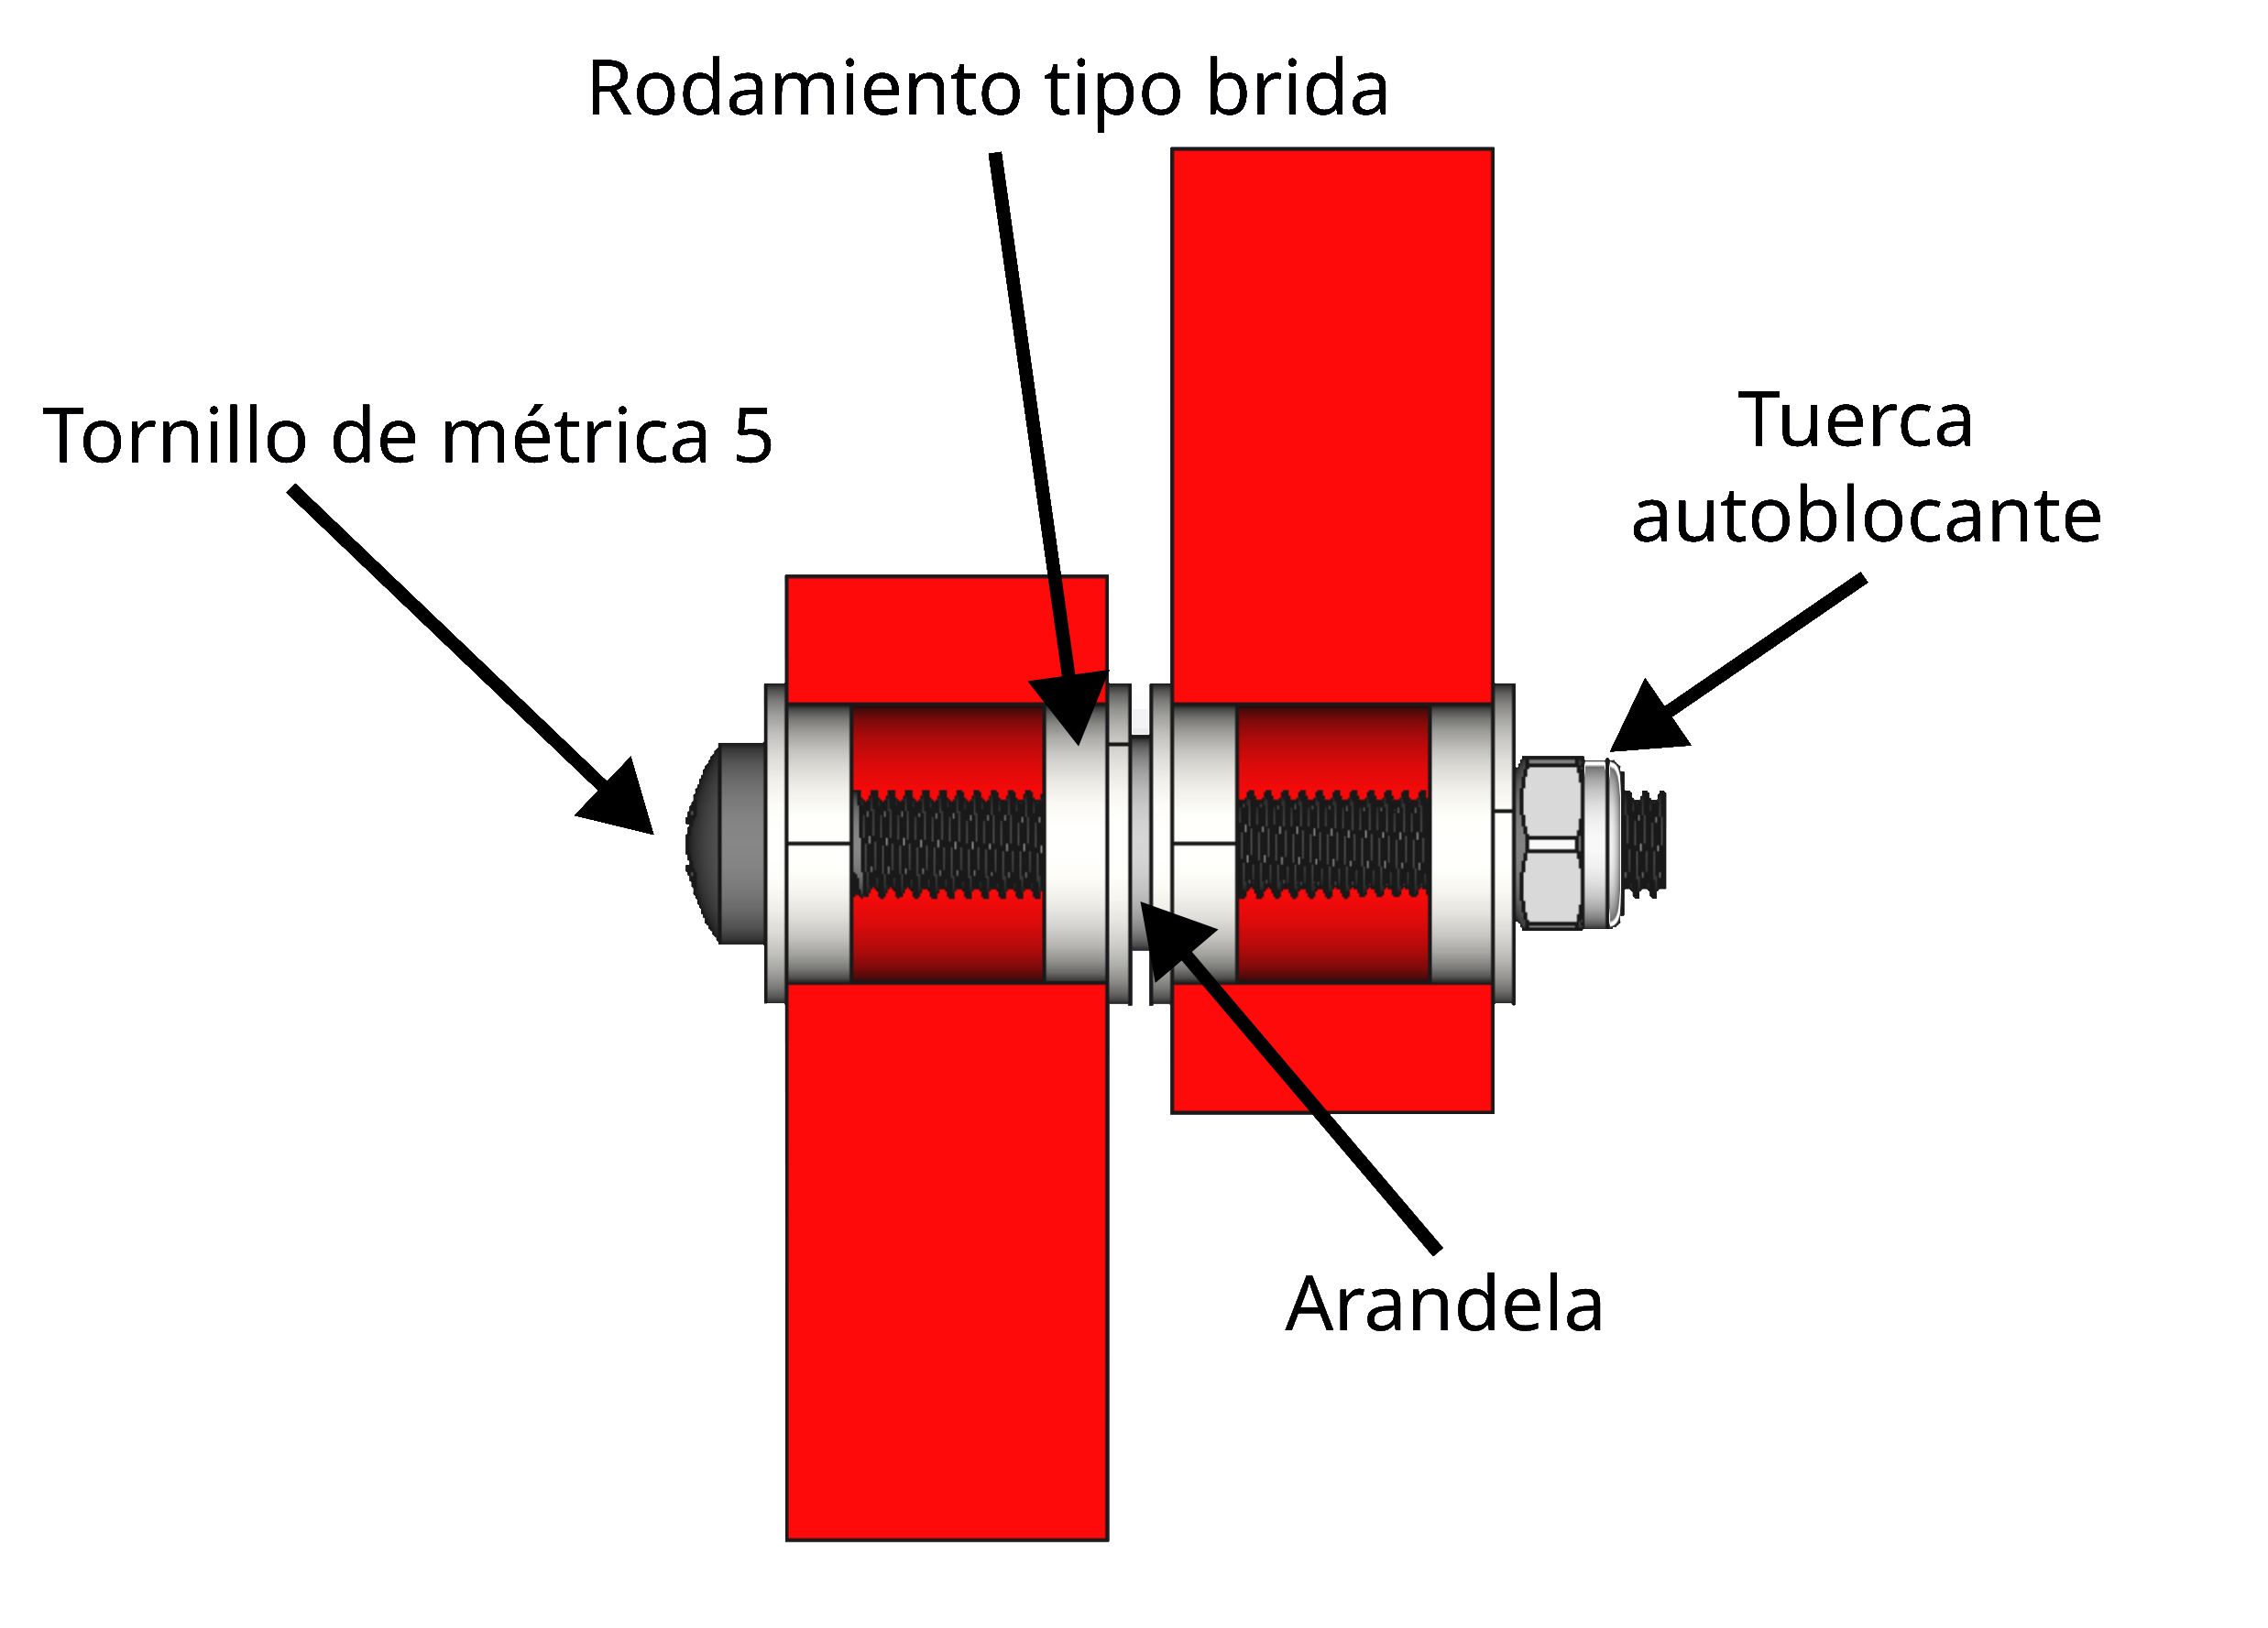
\includegraphics[width=0.5\linewidth ]{figs/RodamientosBrida.png}}
  \caption{Rodamientos de tipo brida}
\end{figure}\ 
\newpage
Estos rodamientos tan particulares son ampliamente usados en las poleas pasivas de las impresoras 3D, por lo 
que son comunes y muy baratos, pudiendo comprar 10 de buena marca por 5\euro.

\subsection{Finales de carrera}
\noindent Este tipo de dispositivos, son usados para conocer el final del recorrido de una articulación y poder establecer así, posiciones 
absolutas.
Existen cantidad de ellos en el mercado con distintos principios de funcionamiento, siendo estos basados en 
\textit{microswitches}\footnote{Interruptor eléctrico de acción rápida y sensible, 
que se activa al aplicar una ligera presión sobre su botón o palanca.} los más baratos. Dentro 
de esta categoría existen diferentes modelos pero se ha optado por el de la Figura \ref{fig:finalcarrera} por ser el más barato y común. Además son 
totalmente compatibles con la placa base elegida anteriormente.

\begin{figure} [ht!]
  \begin{center}
    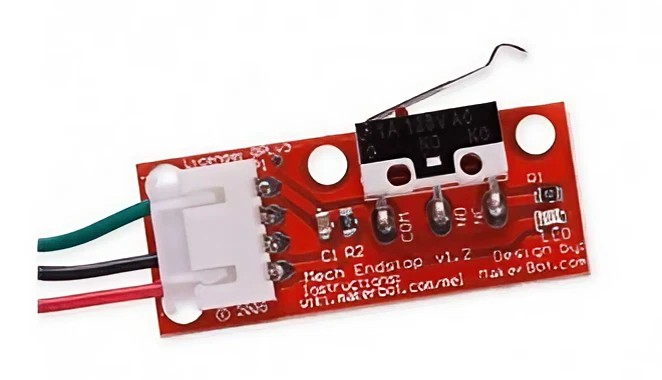
\includegraphics[width=8cm]{figs/finaldecarrera.jpg}
  \end{center}
  \caption{Final de carrera económico}
  \label{fig:finalcarrera}
\end{figure}\ 

\subsection{Electroimán}
\noindent Para llevar a cabo las pruebas, se busca desarrollar una herramienta para el robot, consistente en un electroimán que permita 
el desplazamiento de objetos metálicos. En el mercado, existen diversos tipos de electroimanes con diferentes tamaños y fuerzas. Uno 
especialmente adecuado para esta aplicación es el \textit{D20H15} de la Figura \ref{fig:d20}, cuyo nombre da a entender que tiene un diámetro de 20 mm y una altura de 15 mm. 
Según las especificaciones, es capaz de levantar objetos ferromagnéticos de hasta 3 kg por lo que supera la carga útil que se espera del brazo. Finalmente, 
se ha adquirido la versión de 24 V y 3W por 3\euro.

\begin{figure} [ht!]
  \begin{center}
    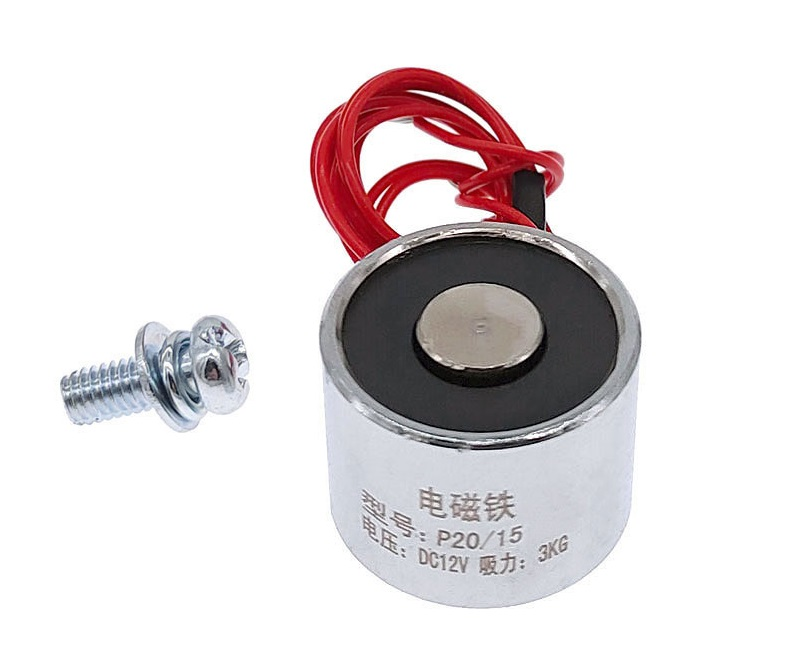
\includegraphics[width=8cm]{figs/d20h15.jpg}
  \end{center}
  \caption{Electroimán D20H15 3KG}
  \label{fig:d20}
\end{figure}\ 


\newpage
\section{Diseño CAD}
\label{sec:di_cad}
\noindent En esta sección se habla de las particularidades del diseño y diversos aspectos a tener en cuenta a la hora de diseñar 
cualquier pieza mecánica que posteriormente será impresa en 3D. 
\\
Para el diseño de este brazo robot, se ha utilizado dos herramientas de diseño. Inicialmente el proyecto se realizó mediante 
la herramienta \textit{Fusion 360} y posteriormente se utilizó \textit{FreeCAD}\ref{subsec:freecad} para cumplir con el objetivo de ser totalmente 
\textit{Open Source} y estar parametrizado, para que cualquier persona pueda investigarlo, modificarlo y utilizarlo de forma gratuita.

\subsection{Base principal}
\noindent Es la parte encargada de unir el resto del robot al suelo. Dentro de ella se encuentra la placa base junto con los controladores 
y toda la electrónica a excepción de la fuente de alimentación. Esto es así debido a que puede ser alimentado de múltiples formas (baterías, 
cargadores de ordenador, fuentes de PC, salidas de alimentación de robots móviles, etc). Además, esta electrónica debe poder estar refrigerada 
por un pequeño ventilador incorporado en la propia base. \\
Se optó por realizar dos piezas circulares y una serie de espaciadores anchos que unían el conjunto, dejando espacio en el interior para 
la placa base. Este tipo de piezas son muy robustas y fáciles de imprimir. 
\begin{figure} [ht!]
  \begin{center}
    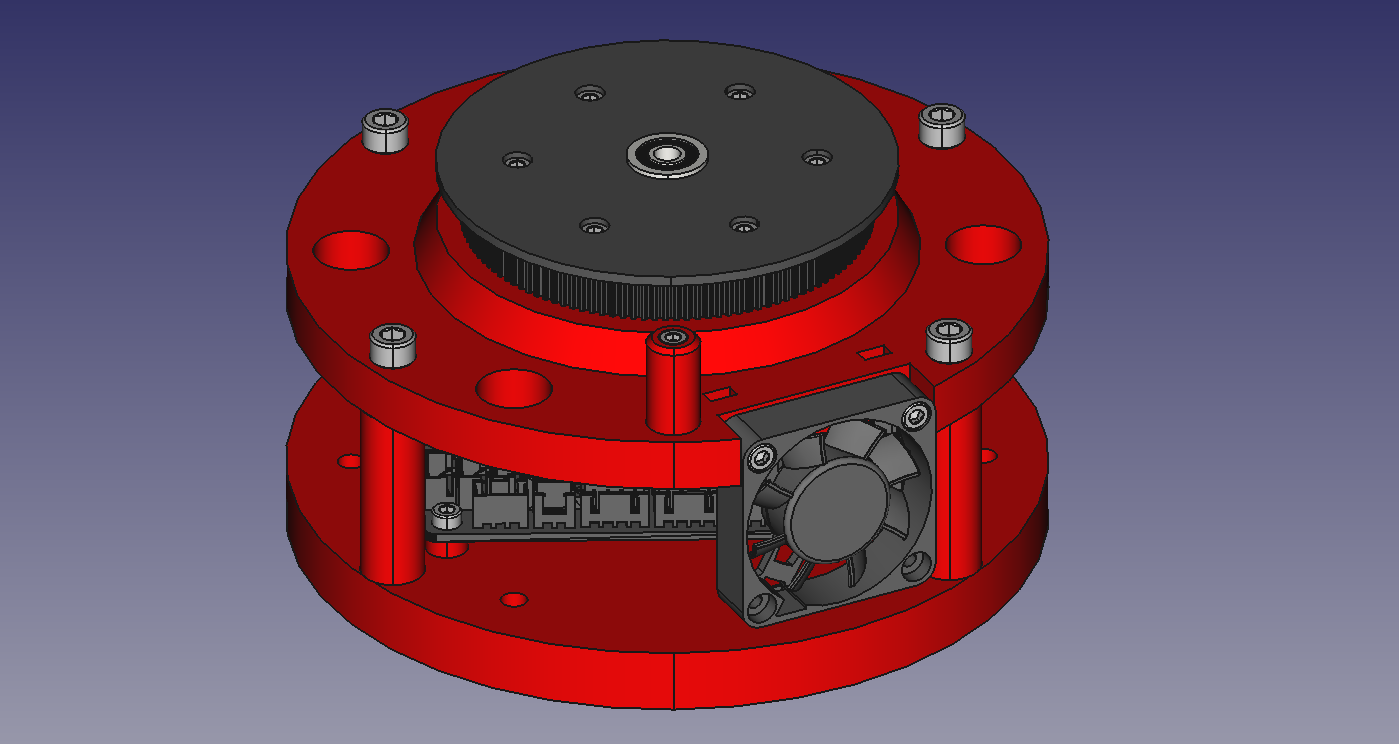
\includegraphics[width=12cm]{figs/base_principal.png}
  \end{center}
  \caption{Base principal}
\end{figure}\ 

\subsubsection{Pieza circular superior}
\noindent La pieza circular superior (Figura \ref{fig:base_principal_superior}), incluye una serie de agujeros y huecos hexagonales para insertar las tuercas M3 que permiten
acoplar la polea de 120 dientes (Figura \ref{fig:base_principal_polea}). Además, incluye un rebaje de 40mm en un lateral para poder insertar y atornillar un ventilador 4010.
\subsubsection{Espaciadores}
\noindent Los espaciadores (Figura \ref{fig:base_principal_espaciadores}) constan de 4 cilindros perforados con un agujero de 5mm por el que entrarán los tornillos de métrica 5.
\subsubsection{Pieza circular inferior}
\noindent La pieza circular inferior (Figura \ref{fig:base_principal_inferior}), contiene una serie de agujeros para poder atornillar la placa base. Además contiene una serie de agujeros en su perímetro 
para poder atornillar el robot al suelo. 

\begin{figure} [ht!]
  \centering    
  \subfigure[Polea 120 dientes]{\label{fig:base_principal_polea}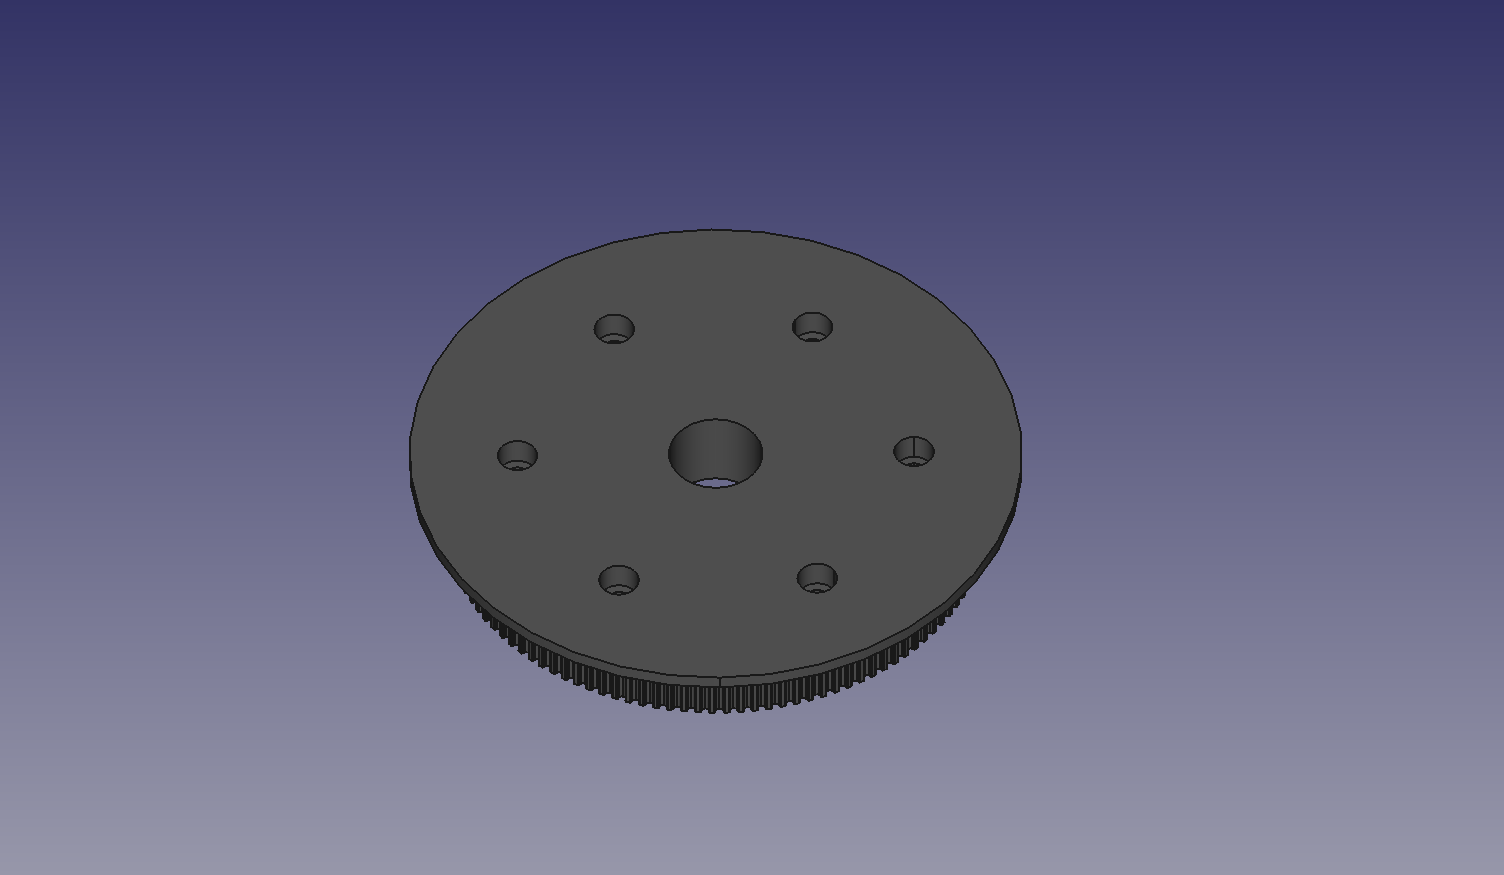
\includegraphics[width=0.45\linewidth ]{figs/base_principal_polea.png}}
  \hspace{1cm}
  \subfigure[Pieza superior]{\label{fig:base_principal_superior}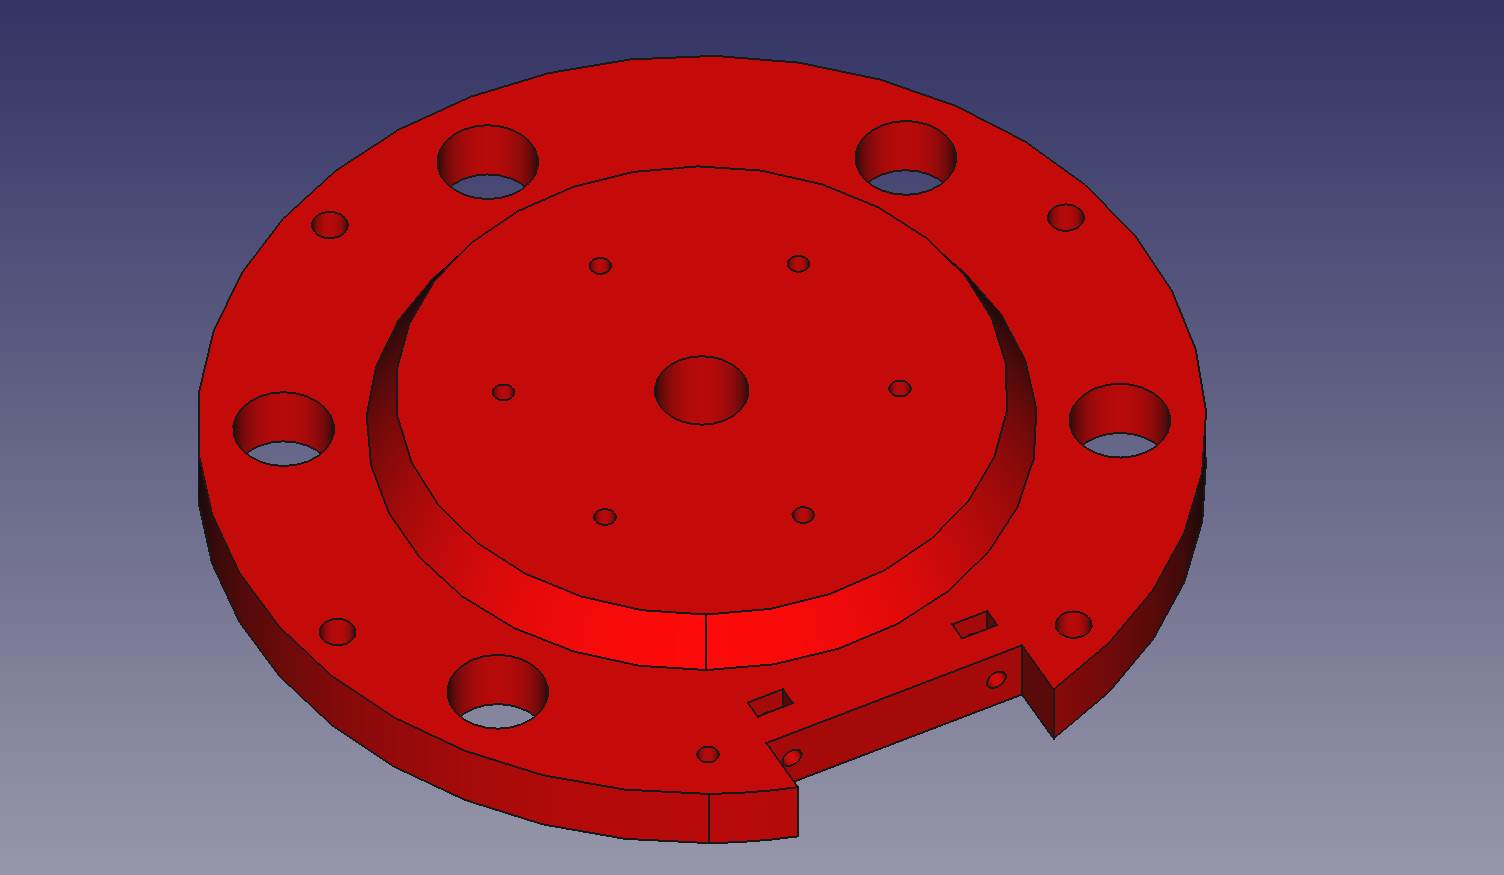
\includegraphics[width=0.45\linewidth]{figs/base_principal_superior.png}}

  \subfigure[Espaciadores]{\label{fig:base_principal_espaciadores}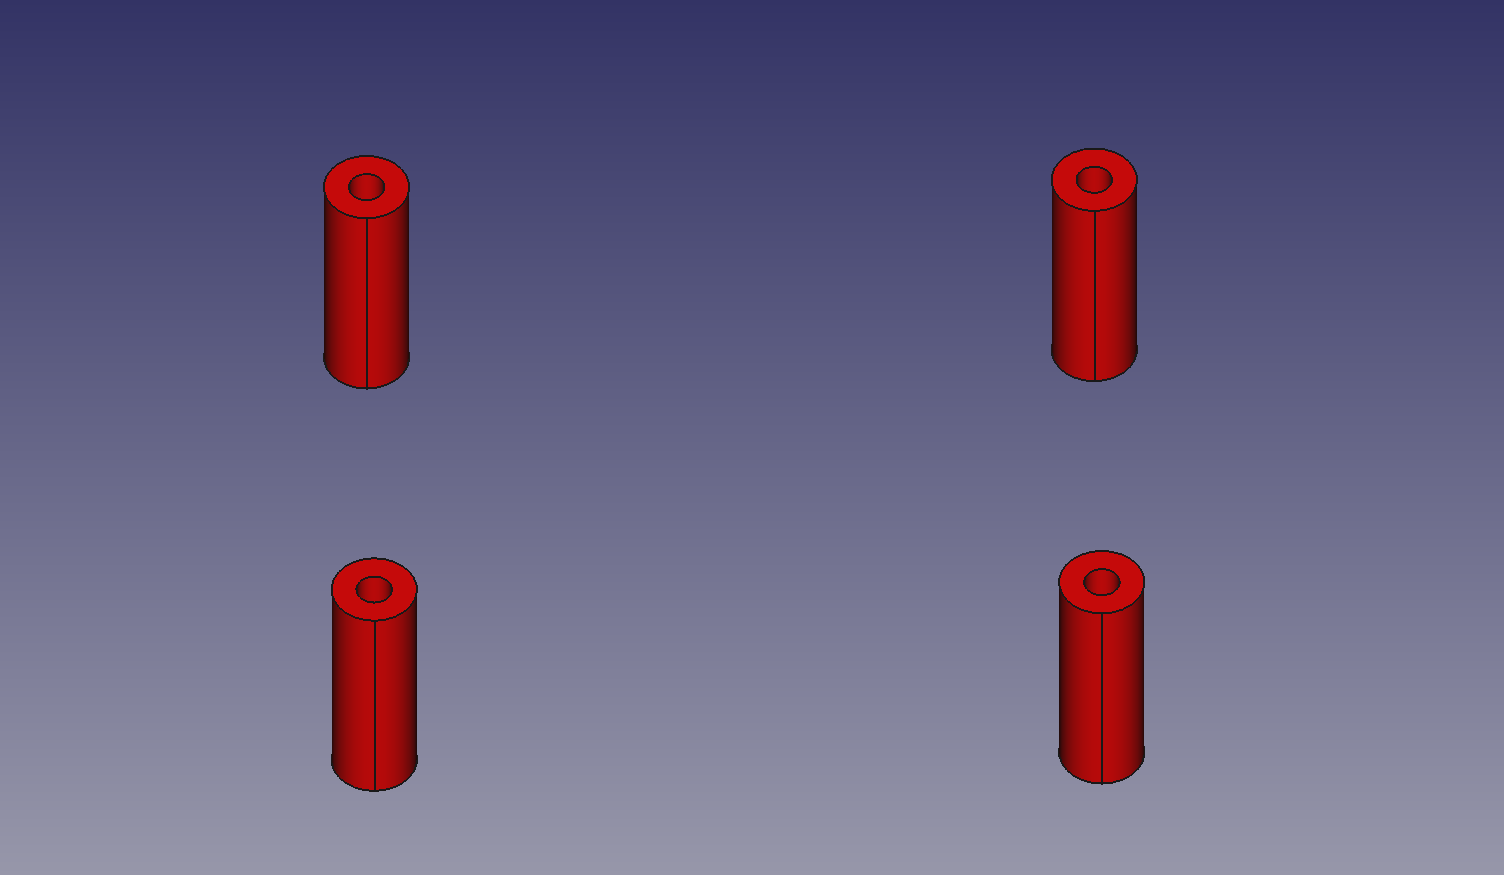
\includegraphics[width=0.45\linewidth]{figs/base_principal_espaciadores.png}}
  \hspace{1cm}
  \subfigure[Pieza inferior]{\label{fig:base_principal_inferior}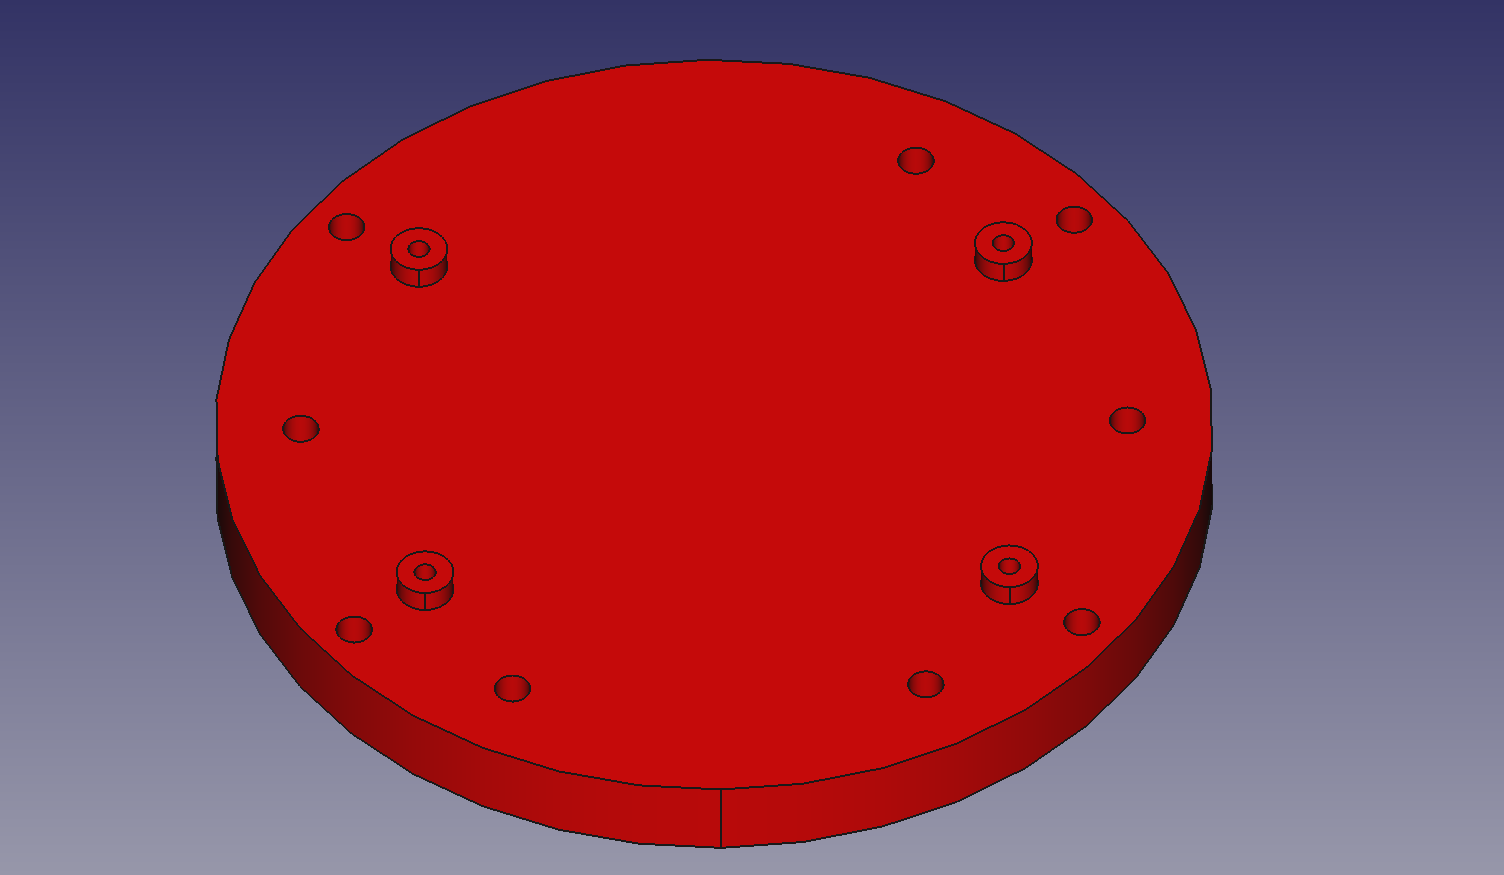
\includegraphics[width=0.45\linewidth]{figs/base_principal_inferior.png}}
\end{figure}
\newpage
\subsection{Base de los motores}
\noindent Este conjunto es el encargado de contener los 3 motores y rotar sobre la base principal. Consiste principalmente en 4 piezas: las dos laterales, la inferior y un espaciador de lado a lado que refuerza el conjunto. Está ideado así 
para solo requerir de piezas planas que serán impresas en dirección horizontal. De esta forma, se logra la mayor resistencia de pieza al incrementar  
la adhesión entre caspas. Además se consigue la máxima exactitud en orificios y formas circulares. Todo el conjunto se une a través de 
varillas roscadas y tuercas (Figura \ref{fig:base_motores}).

\begin{figure} [ht!]
  \begin{center}
    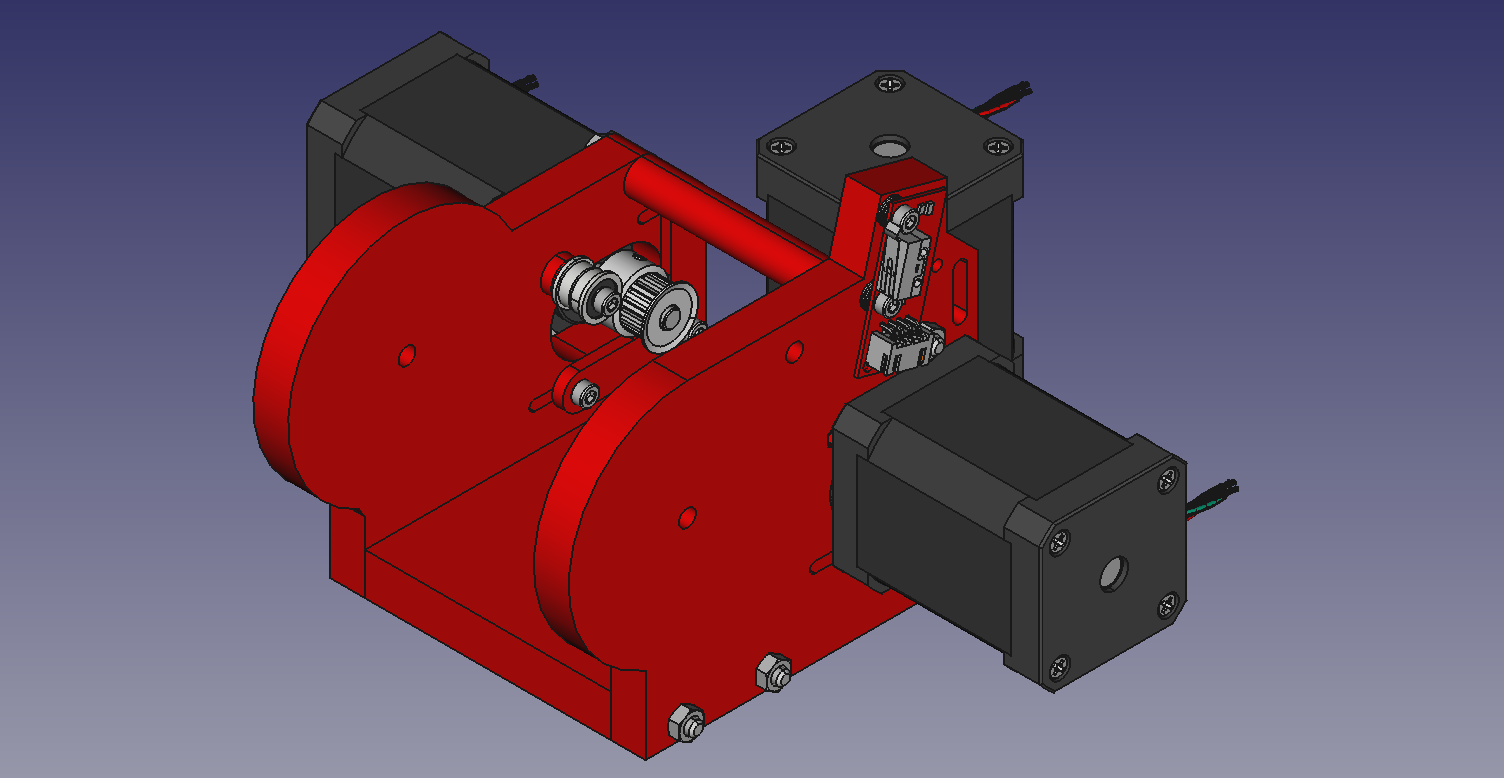
\includegraphics[width=12cm]{figs/base_motores.png}
  \end{center}
  \caption{Base de los motores}
  \label{fig:base_motores}
\end{figure}\ 

Además de esto, cabe destacar el sistema de tensado de las correas, formado por una serie de orificios longitudinales que permiten deslizar el motor 
hasta lograr la tensión óptima, para después fijarse en su sitio. Esto último se realiza mediante una pieza que aumenta la fricción y reparte la presión 
de los 3 tornillos empleados.

Por otra parte, esta pieza incorpora una serie de orificios específicamente creados para acoplar de los 3 finales de carrera del robot. Sumado a ello, 
se ha decidido añadir una serie de ranuras para poder realizar a \textit{posteriori} un manejo de cables más ordenado.

\newpage
\subsection{Paralelogramos}
\noindent Son aquellos elementos descritos en el modelo alámbrico, los cuales han sido modelados en 3D y son los encargados de llevar el 
movimiento de la base de los motores al extremo del robot. 

\begin{figure} [ht!]
  \begin{center}
    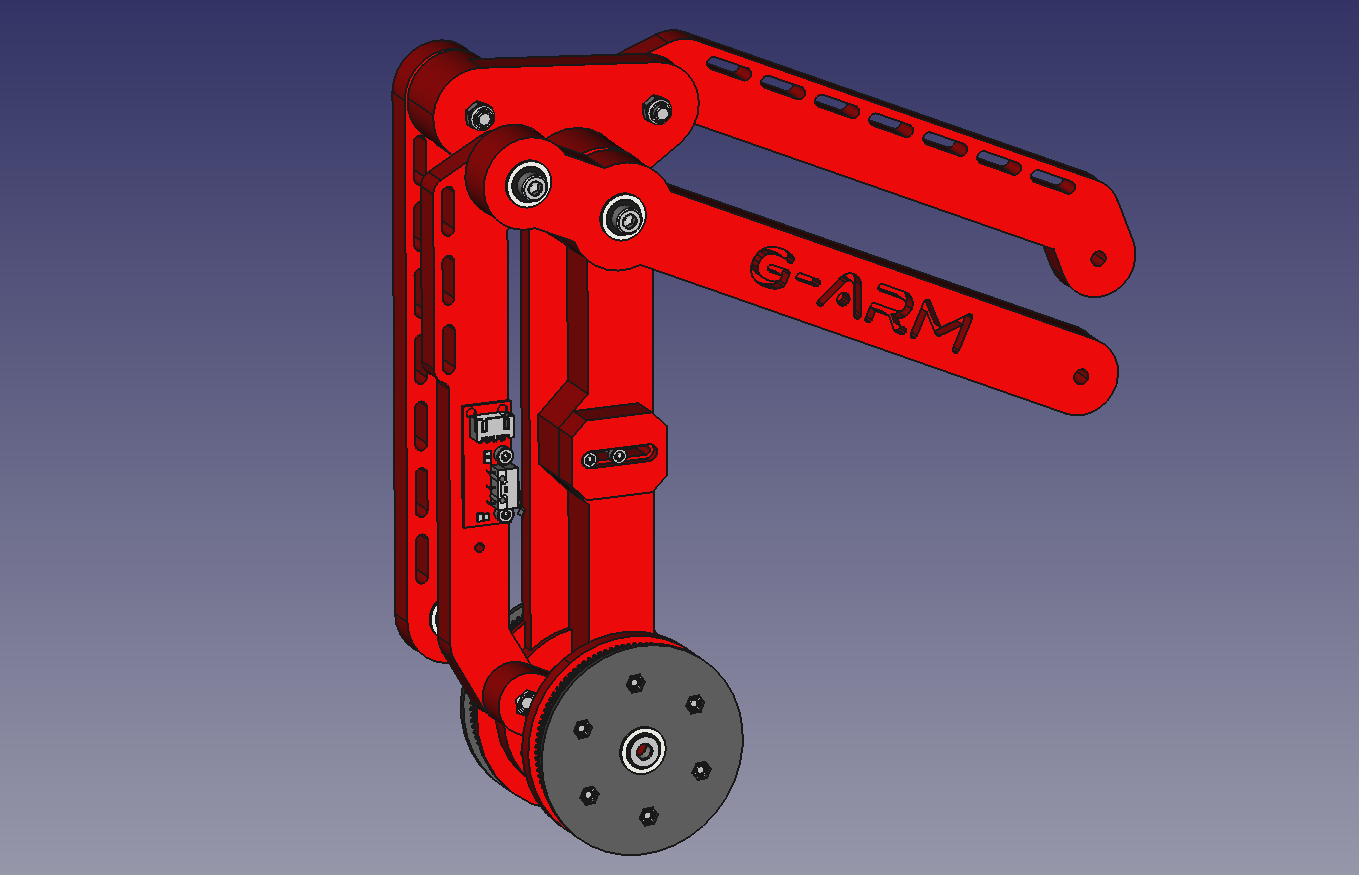
\includegraphics[width=13cm]{figs/links_assembly.png}
  \end{center}
  \caption{Conjunto de los paralelogramos}
  \label{fig:links}
\end{figure}\ 

Como se puede apreciar, algunos de ellos incluyen (al igual que la base de los motores), las ranuras necesarias para poder guiar los cables que van hasta el extremo del 
robot. Además de esto, incorpora el final de carrera en un eslabón, de tal forma que se active al llegar al final de su recorrido. Para poder 
ajustar este punto final, se ha creado el pequeño bloque deslizante de su derecha.

Todas y cada una de las articulaciones incorpora un par de rodamientos brida (presentados en la Sección \ref{sec:bridas}). Estos, deberán ser insertados a 
presión en las piezas reales, por lo que los orificios son ligeramente inferiores al diámetro del rodamiento.

Por otro lado, para la realización de las poleas dentadas GT2, se ha empleado la herramienta paramétrica 
gt2-gear-generator\footnote{\url{https://avtehnik.github.io/gt2-gear-genaretor/}} para generar el contorno de la polea en formato DXF 
(Figura \ref{fig:polea_dxf}). Este formato 
ha sido importado en FreeCAD y extruido gracias a los espacios de trabajo \textit{Draft} y \textit{Part Design}.
\begin{figure} [ht!]
  \begin{center}
    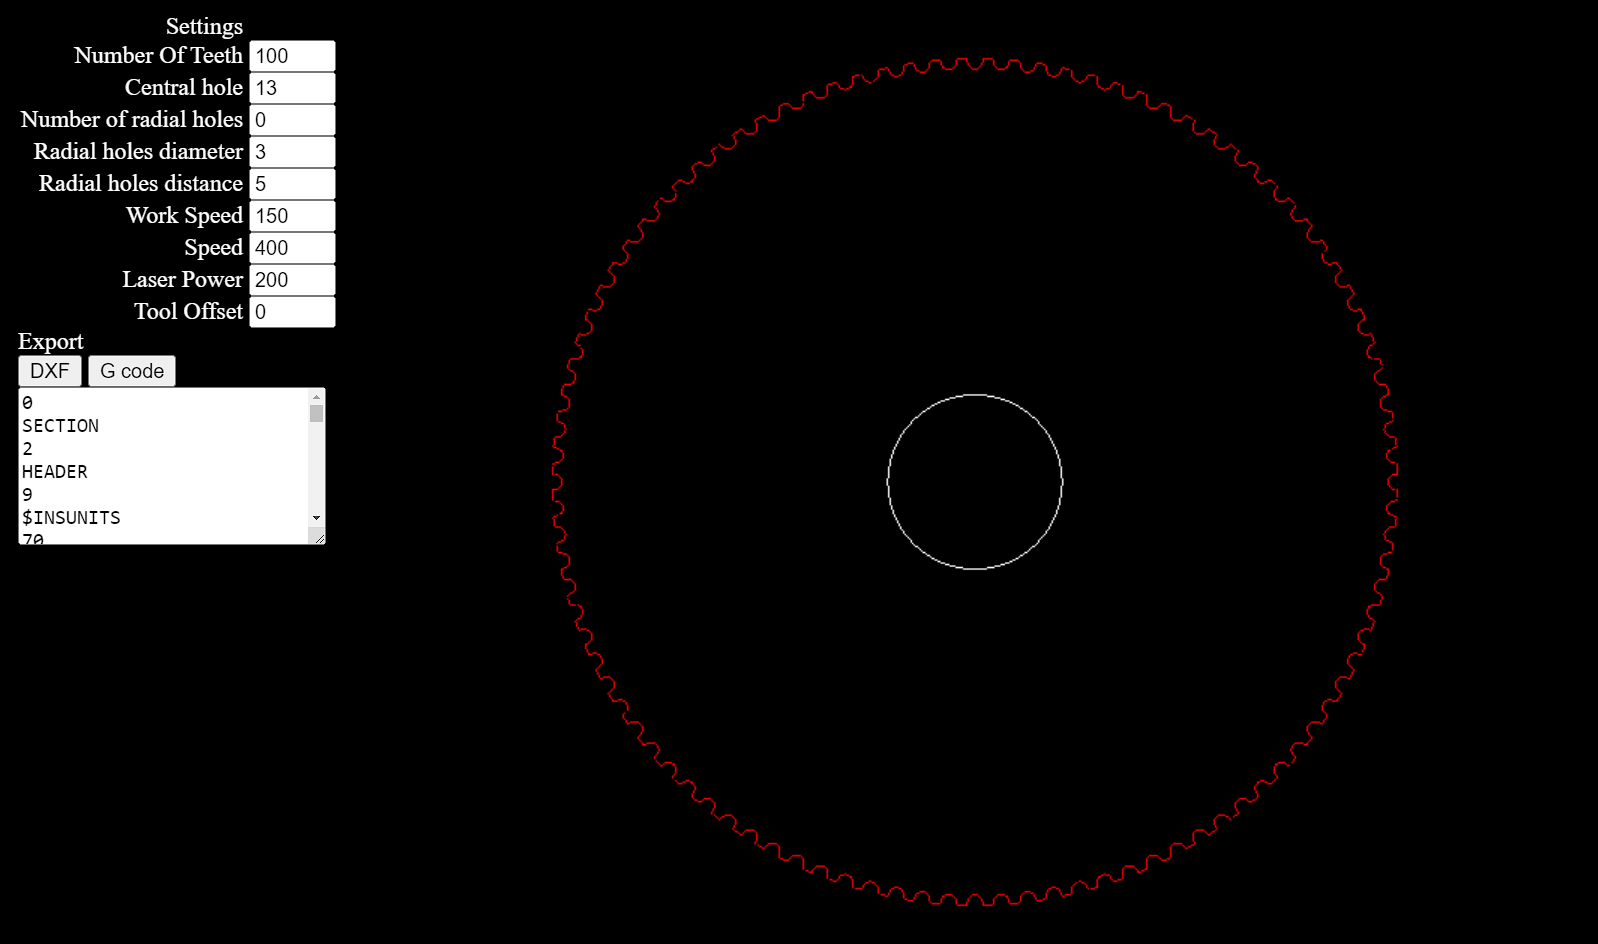
\includegraphics[width=14cm]{figs/dxf_polea.png}
  \end{center}
  \caption{Contorno de la polea de 100 dientes}
  \label{fig:polea_dxf}
\end{figure}\ 

\newpage
Posteriormente, se les ha incluido los agujeros y vaciados hexagonales necesarios para insertar las tuercas de métrica 3, que las unirán a su respectivo eslabón. Mostrados 
en la Figura \ref{fig:polea_show}.
\begin{figure} [ht!]
  \begin{center}
    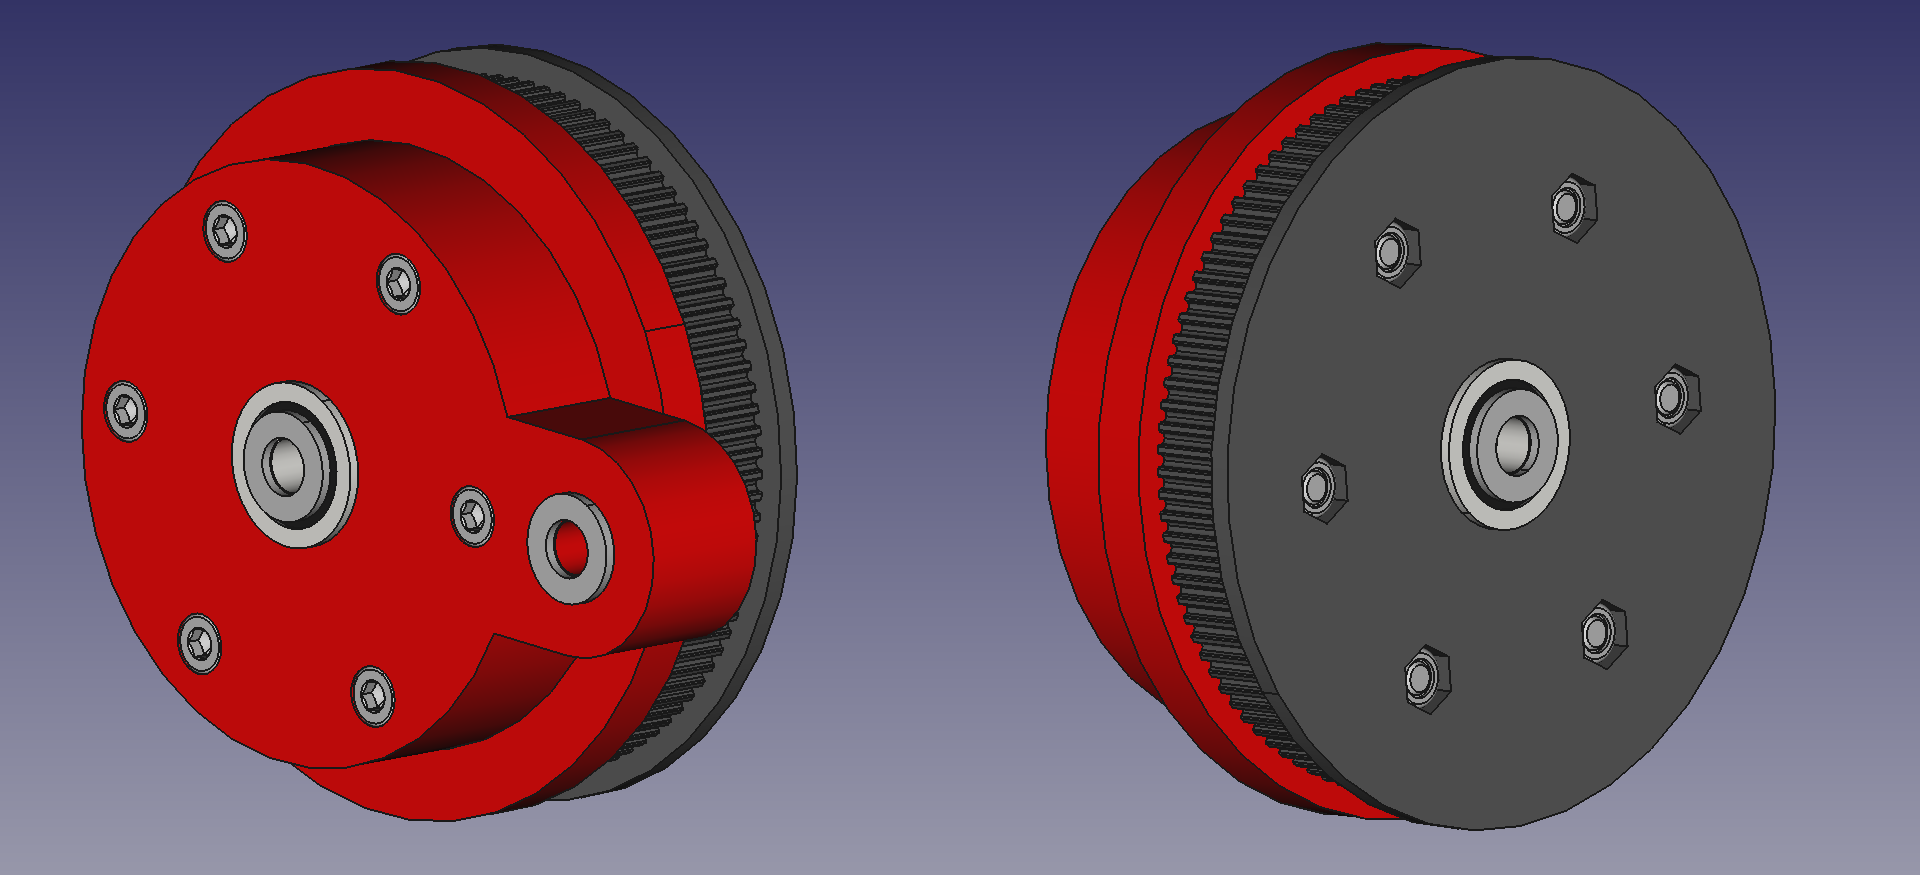
\includegraphics[width=14cm]{figs/polea_show 2.png}
  \end{center}
  \caption{Ambos lados de la palanca de la articulación 3}
  \label{fig:polea_show}
\end{figure}\ 


Finalmente, con el objetivo de personalizar el aspecto del robot, se ha incluido su nombre en el lateral del eslabón más visible.
\newpage
\subsection{Elemento terminal}
\noindent Esta pieza (Figura \ref{fig:extremo_pieza}) está la situada en el extremo del robot. Es la encargada de realizar la unión entre el robot y la herramienta. Por esto, 
se ha ideado con una forma particular que permite acoplar herramientas de una forma sólida e inequívoca. 
\begin{figure} [ht!]
  \begin{center}
    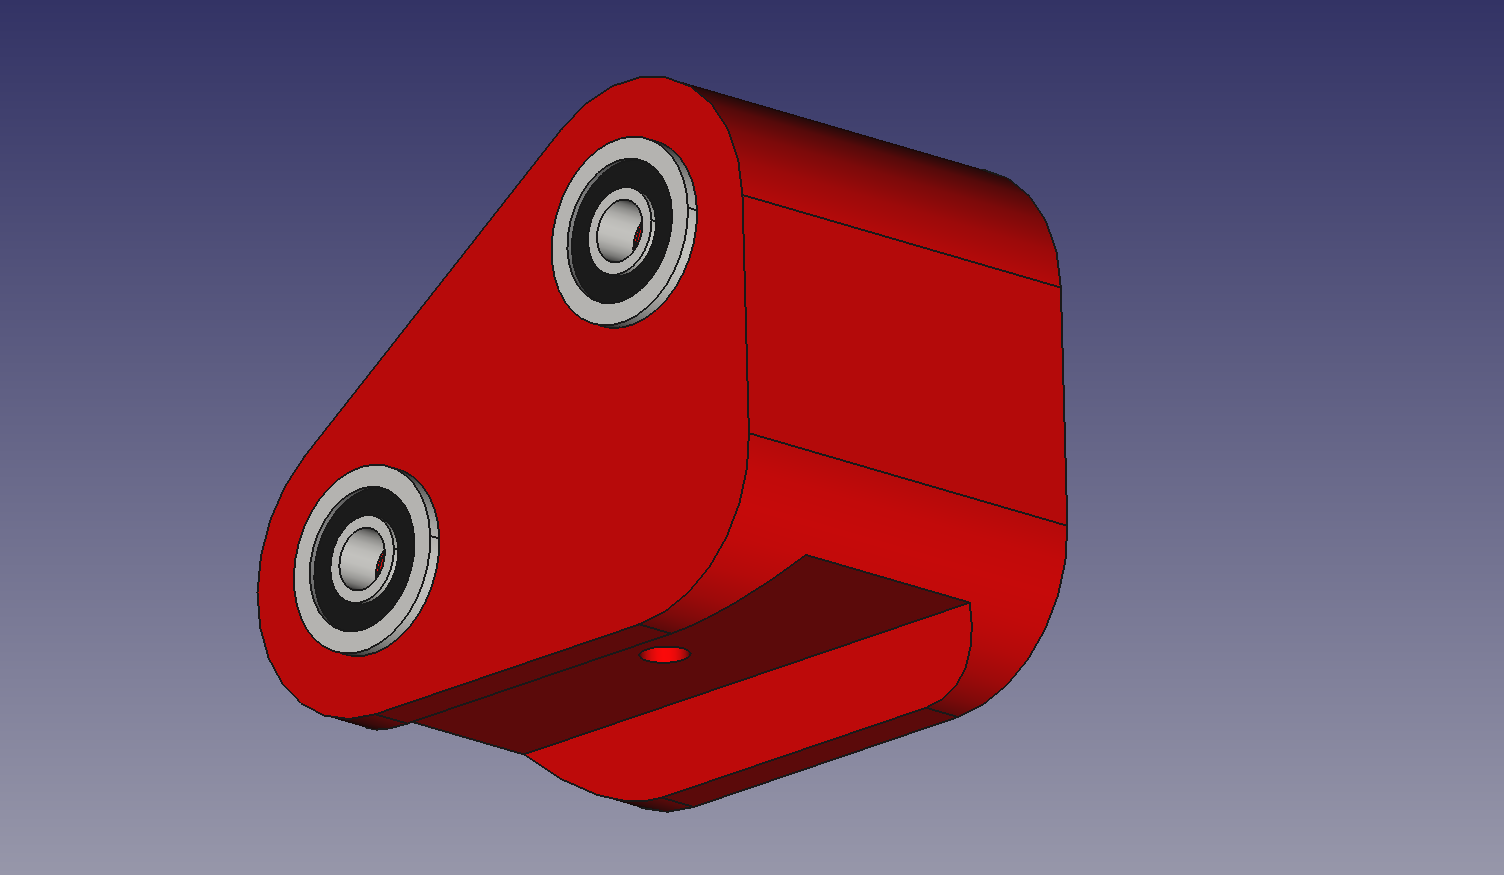
\includegraphics[width=10cm]{figs/extremo_robot.png}
  \end{center}
  \caption{Elemento terminal}
  \label{fig:extremo_pieza}
\end{figure}\ 
\\
Consiste en una acanaladura a 45 grados (Figura \ref{fig:vistas_extremo}) con un agujero que la atraviesa, por el que pasará el tornillo unirá ambas piezas. 
Este acople, diseñado específicamente para este proyecto, es sencillo de usar e impide que la herramienta rote o 
tenga algún tipo de holgura. De hecho, las paredes están en ángulo para obligar a la herramienta a centrarse en la acanaladura y hacer 
la unión muy robusta y precisa.
\begin{figure} [ht!]
  \begin{center}
    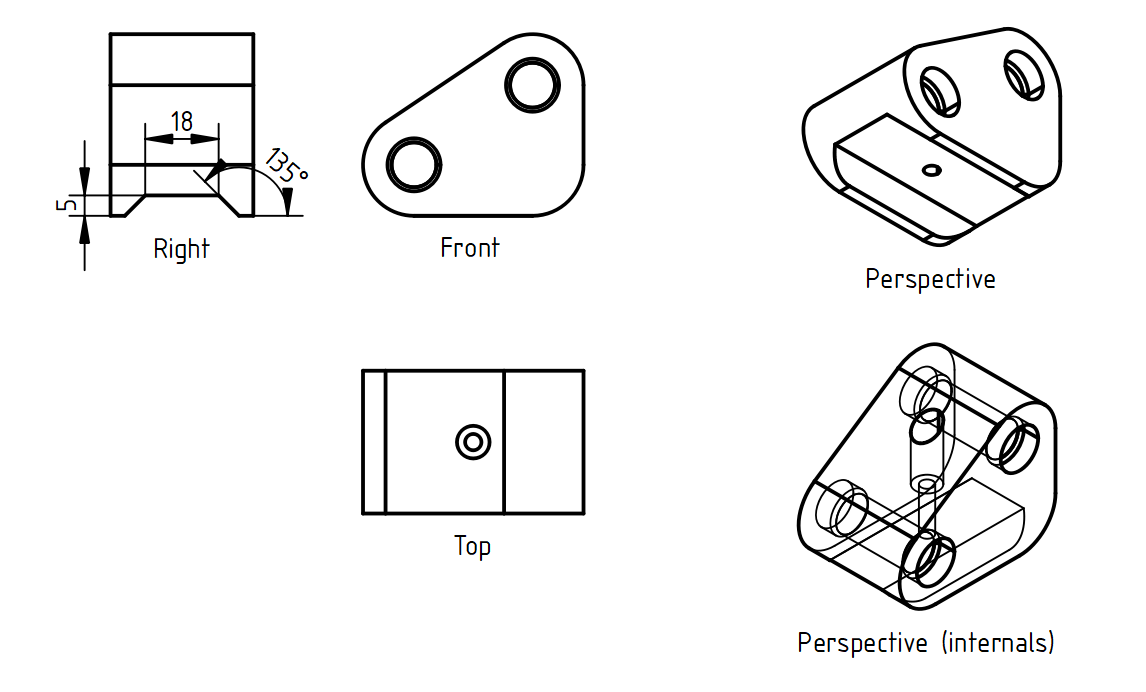
\includegraphics[width=14cm]{figs/vistas_extremo.png}
  \end{center}
  \caption{Vistas del elemento terminal}
  \label{fig:vistas_extremo}
\end{figure}\ 

\subsection{Herramienta electroimán}
\noindent Para dotar al robot de una utilidad, se ha creado una herramienta que contiene el electroimán (Figura \ref{fig:electroiman_pieza}). Esta herramienta debe de tener la forma 
de la acanaladura anterior para poder encajar en el robot. Además se ha redondeado las esquinas para que visualmente se adapte mejor a la 
forma del extremo del robot. Para unir el conjunto se ha utilizado el propio orificio roscado del electroimán, como se puede ver en la Figura 
\ref{fig:electroiman_montaje}

\begin{figure} [ht!]
  \centering    
  \subfigure[Pieza]{\label{fig:electroiman_pieza}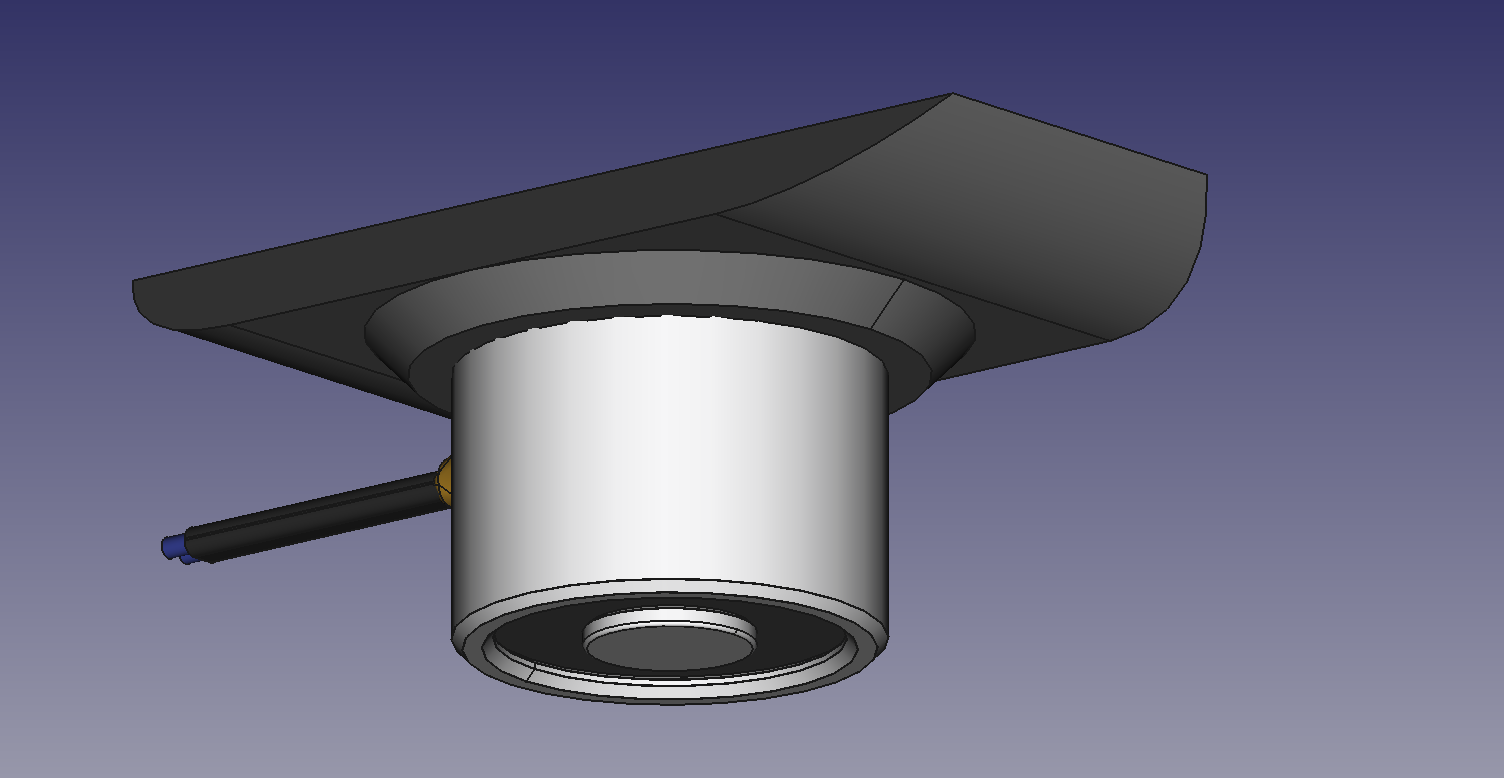
\includegraphics[width=0.8\linewidth ]{figs/electroiman_solo.png}}

  \subfigure[Montaje]{\label{fig:electroiman_montaje}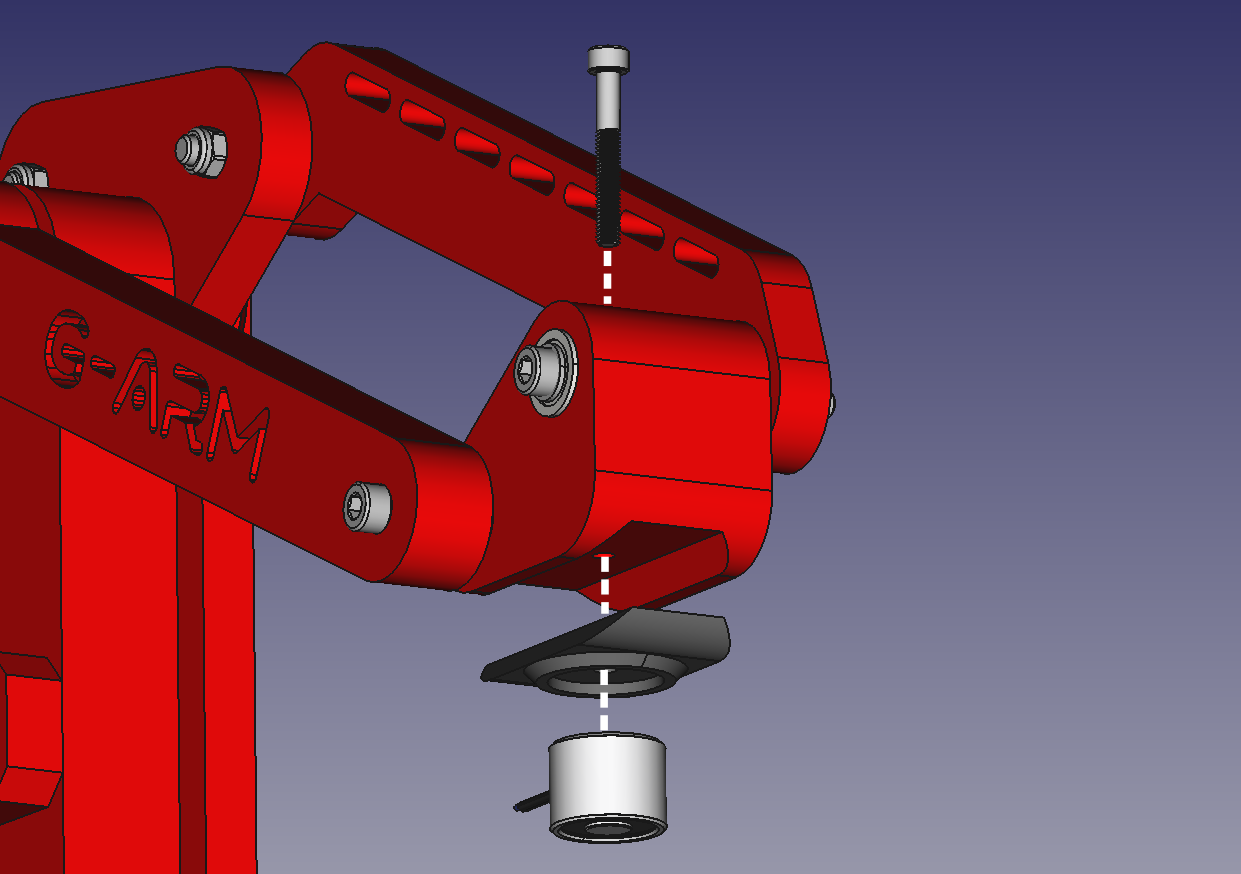
\includegraphics[width=0.8\linewidth]{figs/electroiman_montaje.png}}
  
  \caption{Herramienta electroimán}
\end{figure}

\newpage
\section{Impresión y montaje}
\noindent En esta sección se exponen todos los detalles a tener en cuenta a la hora de querer replicar este proyecto. Para la impresión 
de G-Arm se ha utilizado una impresora Ender-3 Pro\footnote{\url{https://www.creality.com/products/ender-3-pro-3d-printer}} y un rollo 
de 1Kg de filamento PLA Rojo convencional.
\begin{figure} [h!]
\begin{center}
  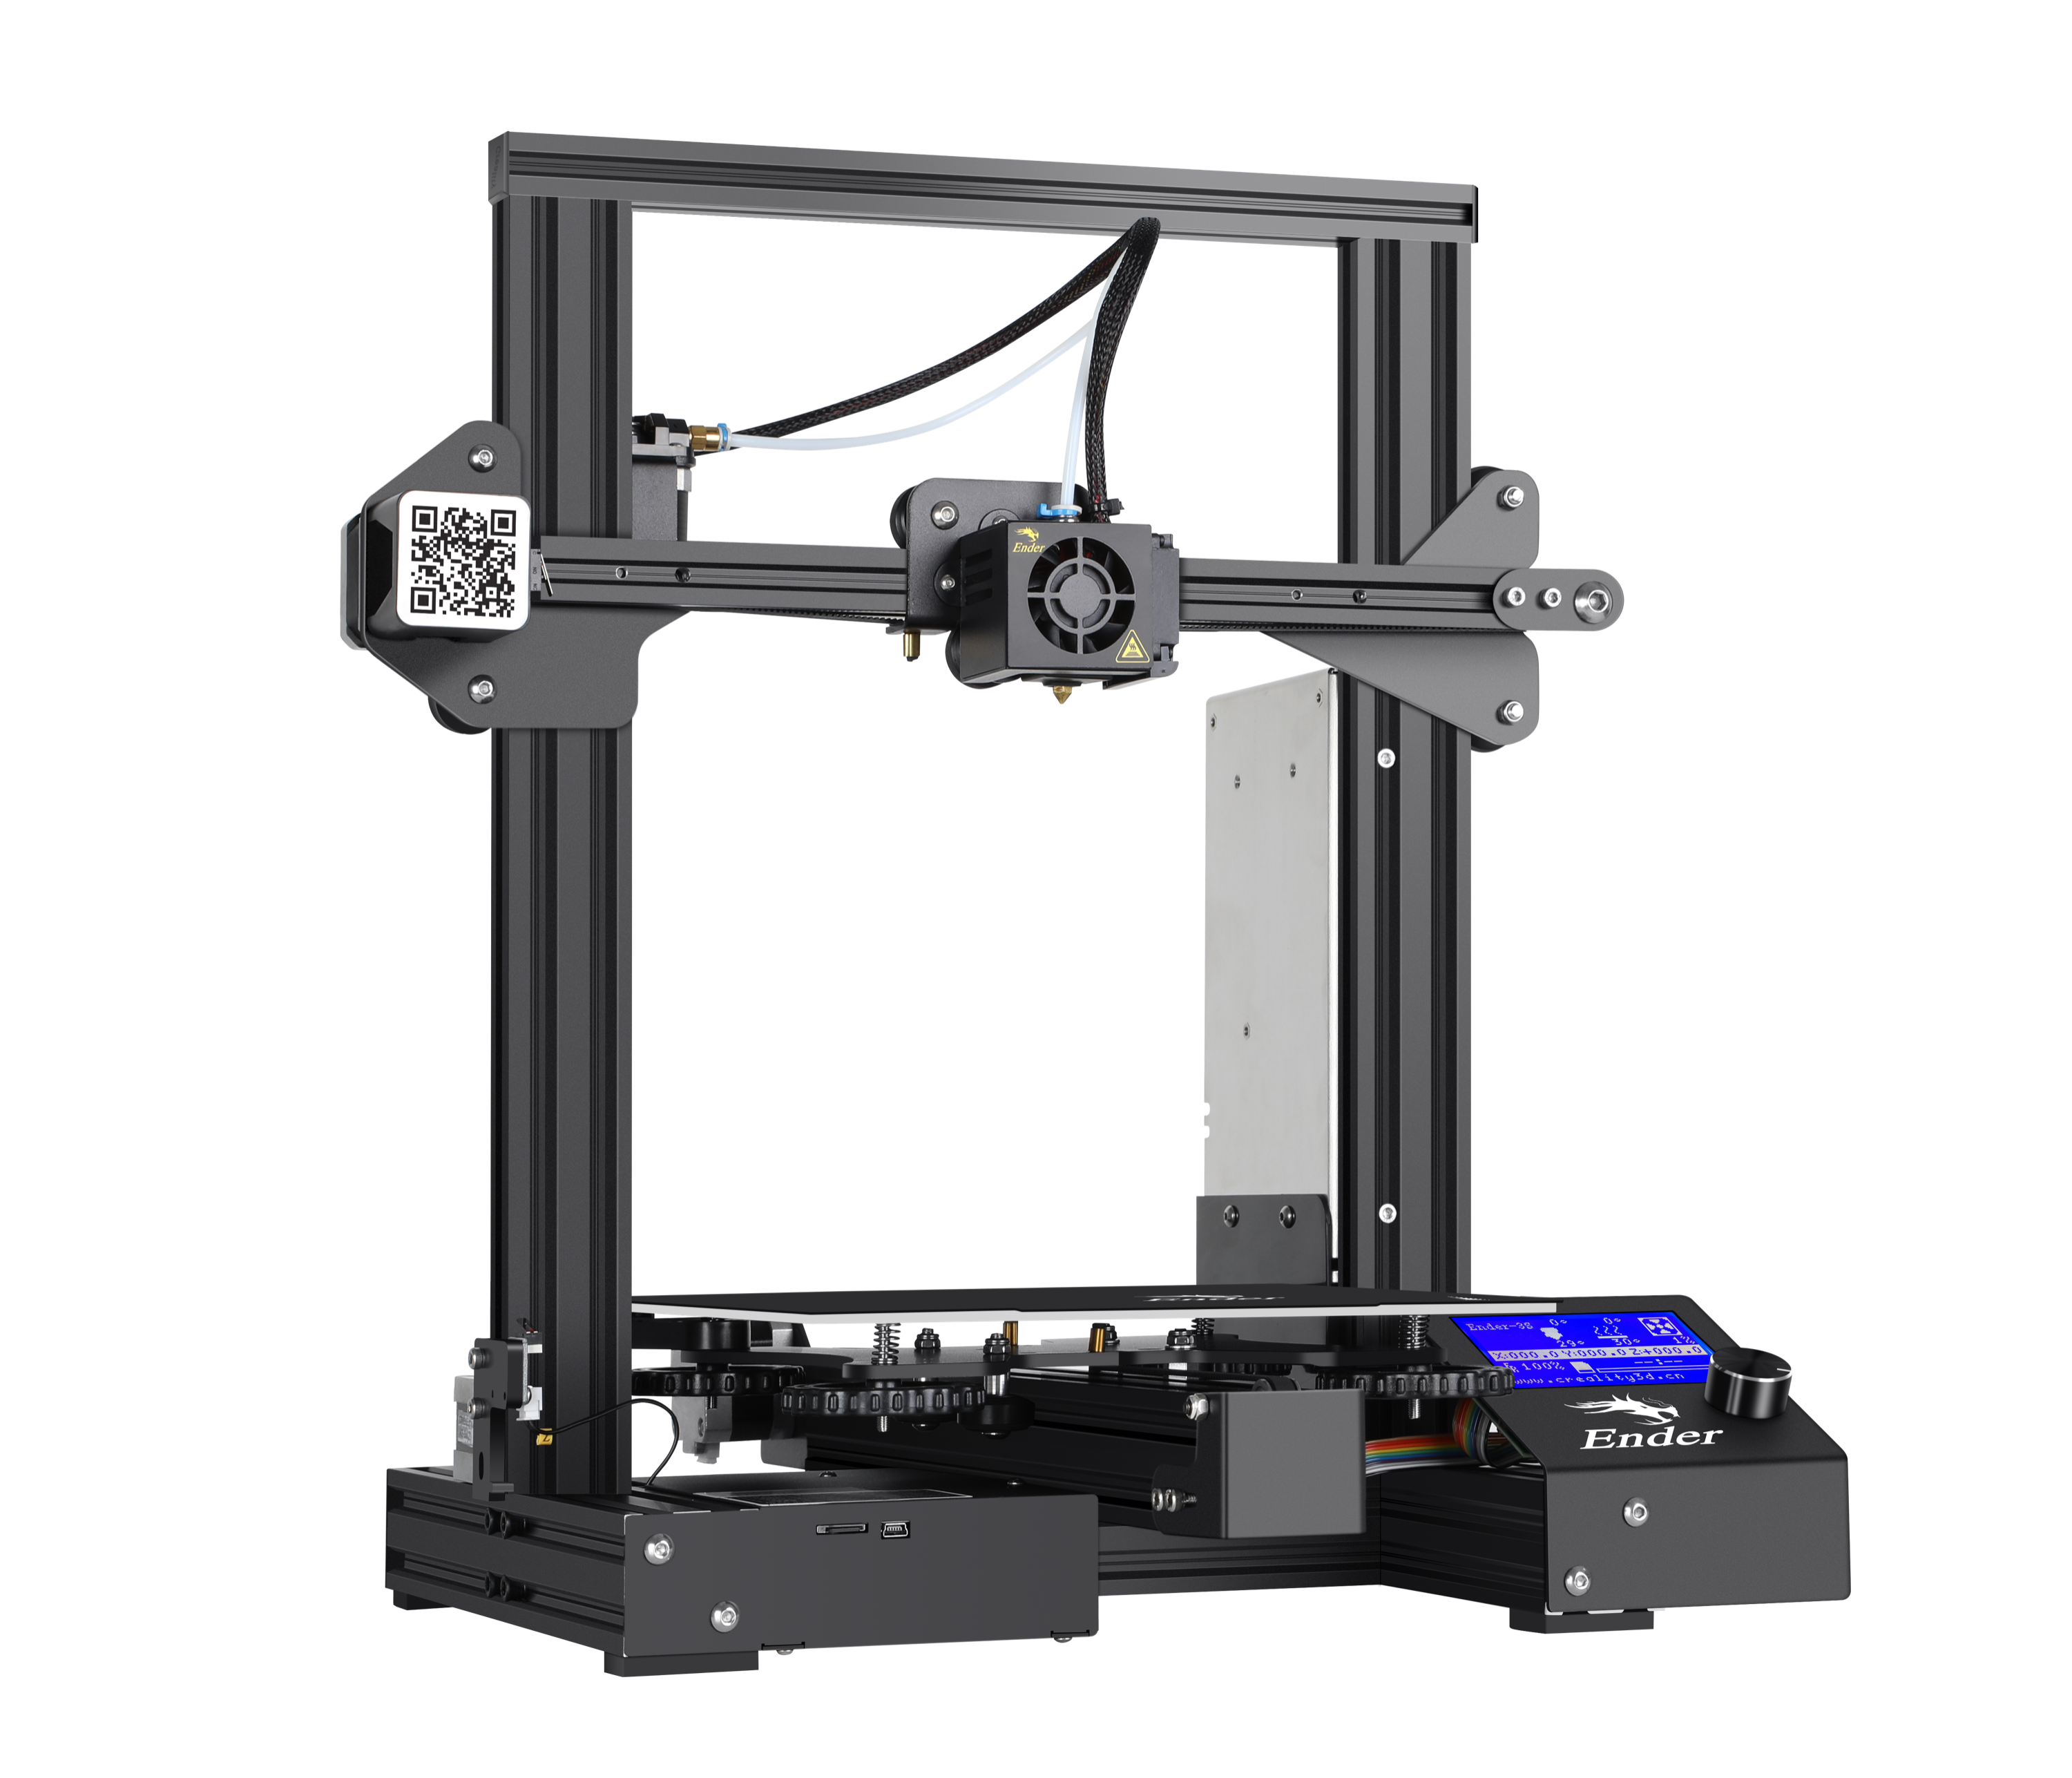
\includegraphics[width=8cm]{figs/ender3.png}
\end{center}
\caption{Ender-3 Pro V1 2017}
\label{fig:ender3pro}
\end{figure}\   

Con la intención de lograr la mejor organización posible, se ha decidido incluir una serie de tablas 
detallando los componentes necesarios para el montaje del robot. En la Tabla \ref{cuadro:componentes} se listan aquellos 
componentes que deben ser comprados y su precio. Se recomienda adquirirlos a través de páginas como \textit{Aliexpress} ya que 
resulta significativamente más barato que comprarlos a través de \textit{Amazon}. Por otro lado, es necesaria la tornillería 
de las Tablas \ref{cuadro:tornillos}, \ref{cuadro:tuercas}, \ref{cuadro:arandelas} y \ref{cuadro:varillas}, comprada en ferreterías locales y nacionales como \textit{Randrade} (Online). El resto 
de piezas detalladas en la Tabla \ref{cuadro:piezas}, son enteramente imprimibles en 3D. Se recomienda configurar el laminador 
con las densidades de relleno propuestas en dicha tabla. Cada pieza está diferenciada con un número y se pueden requerir varias 
unidades de una misma pieza (indicado en la propia tabla). Se recomienda utilizar una altura de capa de 0.12mm y tres líneas 
de grosor de pared.
\begin{table}[H]
\begin{center}
\begin{tabular}{|c|c|c|c|}
\hline
\textbf{Componente} & \textbf{Modelo} & \textbf{Cantidad} & \textbf{Precio total} \\
\hline
Motor Nema 17 & 17HS24-2104S & 3 & 56\euro \\
Controlador & TMC2209 & 3 & 10\euro \\
Placa base & MKS DLC32 & 1 & 16\euro \\
Final de carrera & MakerBot (rojo) & 3 & 5\euro \\
Fuente de alimentación & 24V 5A (opcional)\ref{subsec:fuente_alimentacion} & 1 & 15\euro \\
Rodamiento &  F695-2RS Fushi & 22 & 15\euro \\
Rodamiento & F623RS Fushi & 6 & 5.5\euro \\
Polea GT2 & Correa:6mm ID:5mm & 3 & 1.5\euro \\
Correa GT2 & Correa:6mm Largo:252mm & 2 & 3.5\euro \\ 
Correa GT2 &  Correa:6mm Largo:280mm & 1 & 1.8\euro \\ 
Ventilador & 24V 4010 & 1 & 2\euro \\
Electroimán & D20H15mm 3KG 24V & 1 & 3\euro \\
Plástico para imprimir & PLA/PETG 1Kg & 1 & 22\euro \\
\hline
\end{tabular}
\caption{Componentes hardware necesarios}
\label{cuadro:componentes}
\end{center}
\end{table}

\begin{table}[H]
  \begin{center}
  \begin{tabular}{|c|c|c|}
  \hline
  \textbf{Métrica} & \textbf{Tamaño} & \textbf{Cantidad} \\
  \hline
  M3 & 12mm & 8\\
  M3 & 16mm & 11\\
  M3 & 20mm & 10\\
  M3 & 25mm & 13\\
  M4 & 30mm & 3\\
  M5 & 25mm & 1\\
  M5 & 30mm & 3\\
  M5 & 40mm & 1\\
  M5 & 50mm & 5\\
  M5 & 55mm & 1\\
  M5 & 60mm & 2\\
  
  \hline
  \end{tabular}
  \caption{Tornillos necesarios}
  \label{cuadro:tornillos}
  \end{center}
  \end{table}

\begin{table}[H]
\begin{center}
\begin{tabular}{|l|c|}
\hline
\textbf{Métrica} & \textbf{Cantidad} \\
\hline
M3 normal & 6\\
M3 autoblocante & 29\\
M4 autoblocante & 8\\
M5 normal & 5\\
M5 autoblocante & 10\\

\hline
\end{tabular}
\caption{Tuercas necesarias}
\label{cuadro:tuercas}
\end{center}
\end{table}

\begin{table}[H]
  \begin{center}
  \begin{tabular}{|c|c|}
  \hline
  \textbf{Métrica} & \textbf{Cantidad} \\
  \hline
  M3 & 29\\
  M5 & 16\\
  \hline
  \end{tabular}
  \caption{Arandelas necesarias}
  \label{cuadro:arandelas}
  \end{center}
  \end{table}
  
  \begin{table}[H]
    \begin{center}
    \begin{tabular}{|c|c|}
    \hline
    \textbf{Métrica} & \textbf{Cantidad} \\
    \hline
    M3 & 1 metro\\
    M4 & 1 metro\\
    M5 & 1 metro\\
  
    \hline
    \end{tabular}
    \caption{Varillas roscadas necesarias}
    \label{cuadro:varillas}
    \end{center}
    \end{table}


\begin{table}[H]
  \begin{center}
  \begin{tabular}{|c|c|c|}
  \hline
  \textbf{Identificador} & \textbf{Cantidad} & \textbf{Relleno óptimo} \\
  \hline
  \#1 Base inferior & 1 & 15\% \\
  \hline
  \#2 Espaciador de la base & 4 & 100\% \\
  \hline
  \#3 Base superior & 1 & 15\% \\
  \hline
  \#4 Polea 120T & 1 & 20\% \\
  \hline
  \#5 Base de los motores & 1 & 15\% \\
  \hline
  \#6 Límite de la base & 1 & 100\% \\
  \hline
  \#7 Lateral derecho & 1 & 15\% \\
  \hline
  \#8 Lateral izquierdo & 1 & 15\% \\
  \hline
  \#9 Espaciador de rodamiento & 3 & 100\% \\
  \hline
  \#10 Polea 100T & 2 & 20\% \\
  \hline
  \#11 Eslabón 1 & 1 & 15\% \\
  \hline
  \#12 Espaciador de motores & 1 & 100\% \\
  \hline
  \#13 Tope de correa & 1 & 15\% \\
  \hline
  \#14 Palanca articulación 2 & 1 & 20\% \\
  \hline
  \#15 Paralelo eslabón 1 & 1 & 15\% \\
  \hline
  \#16 Paralelo del extremo & 1 & 15\% \\
  \hline
  \#17 Codo & 1 & 15\% \\
  \hline
  \#18 Ajuste de límite & 1 & 15\% \\
  \hline
  \#19 Eslabón 2 & 1 & 15\% \\
  \hline
  \#20 Paralelo eslabón 2 & 1 & 15\% \\
  \hline
  \#21 Extremo del robot & 1 & 15\% \\
  \hline
  \#22 Fijador de motores & 2 & 100\% \\
  \hline
  \#23 Herramienta electroimán & 1 & 15\% \\
  \hline
  \end{tabular}
  \caption{Piezas necesarias}
  \label{cuadro:piezas}
  \end{center}
  \end{table}
  

El precio total de los componentes necesarios es de 156.3\euro{} sumado a unos 15 en tornillería, hacen un coste total aproximado de 171\euro.\\

La impresión de todas las piezas puede llevar cerca de 60 horas. En cambio, 
el montaje requiere de apenas 2, o incluso, menos dependiendo de la habilidad del usuario. Para saber la posición de cada pieza 
y dónde montarla, se recomienda consultar el montaje 
completo\footnote{\url{https://github.com/RoboticsURJC/tfg-vperez/blob/280861172bce3b1c0cfbb155a434364ea68eeb30/src/design/FreeCad/\%230\_ASSEMBLY.FCStd}} 
realizado mediante A2Plus en FreeCAD (Figura \ref{fig:montaje_freeacd_a2plus}). En él, se puede ver 
el nombre de cada pieza, tornillo necesario y posición.
\begin{figure} [h!]
  \begin{center}
    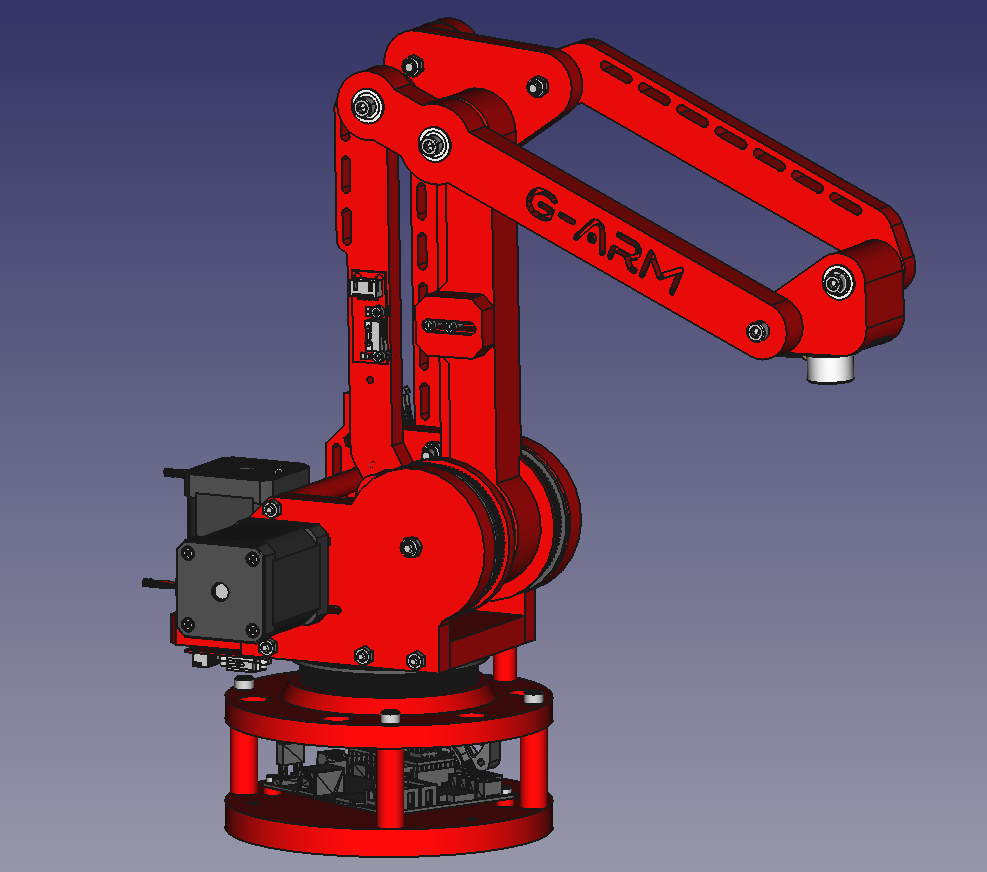
\includegraphics[width=14cm]{figs/montaje.png}
  \end{center}
  \caption{Ensamble CAD completo del robot final}
  \label{fig:montaje_freeacd_a2plus}
  \end{figure}\   

En cuanto al montaje de la electrónica es realmente sencillo debido a que existen numerosos tutoriales 
y manuales en internet que utilizan esta placa. Por si no fuera poco, el propio circuito impreso de la 
placa tiene serigrafiado un nombre en cada conector. El único aspecto a tener en cuenta es la regulación 
de corriente de los 3 controladores TMC2209. Esta se realiza mediante un pequeño potenciómetro y requiere 
de un multímetro para leer los valores. En este \href{https://all3dp.com/2/vref-calculator-tmc2209-tmc2208-a4988/}{enlace} se muestra un tutorial de como hacerlo.  
\newpage
En la Figura \ref{fig:montaje_real} se muestra el resultado real del robot. Como es obvio es idéntico al realizado en el diseño CAD y resulta robusto 
y estable. La organización de los cables ha resultado sencilla debido a las ranuras añadidas en la fase de diseño.
\begin{figure} [h!]
  \begin{center}
    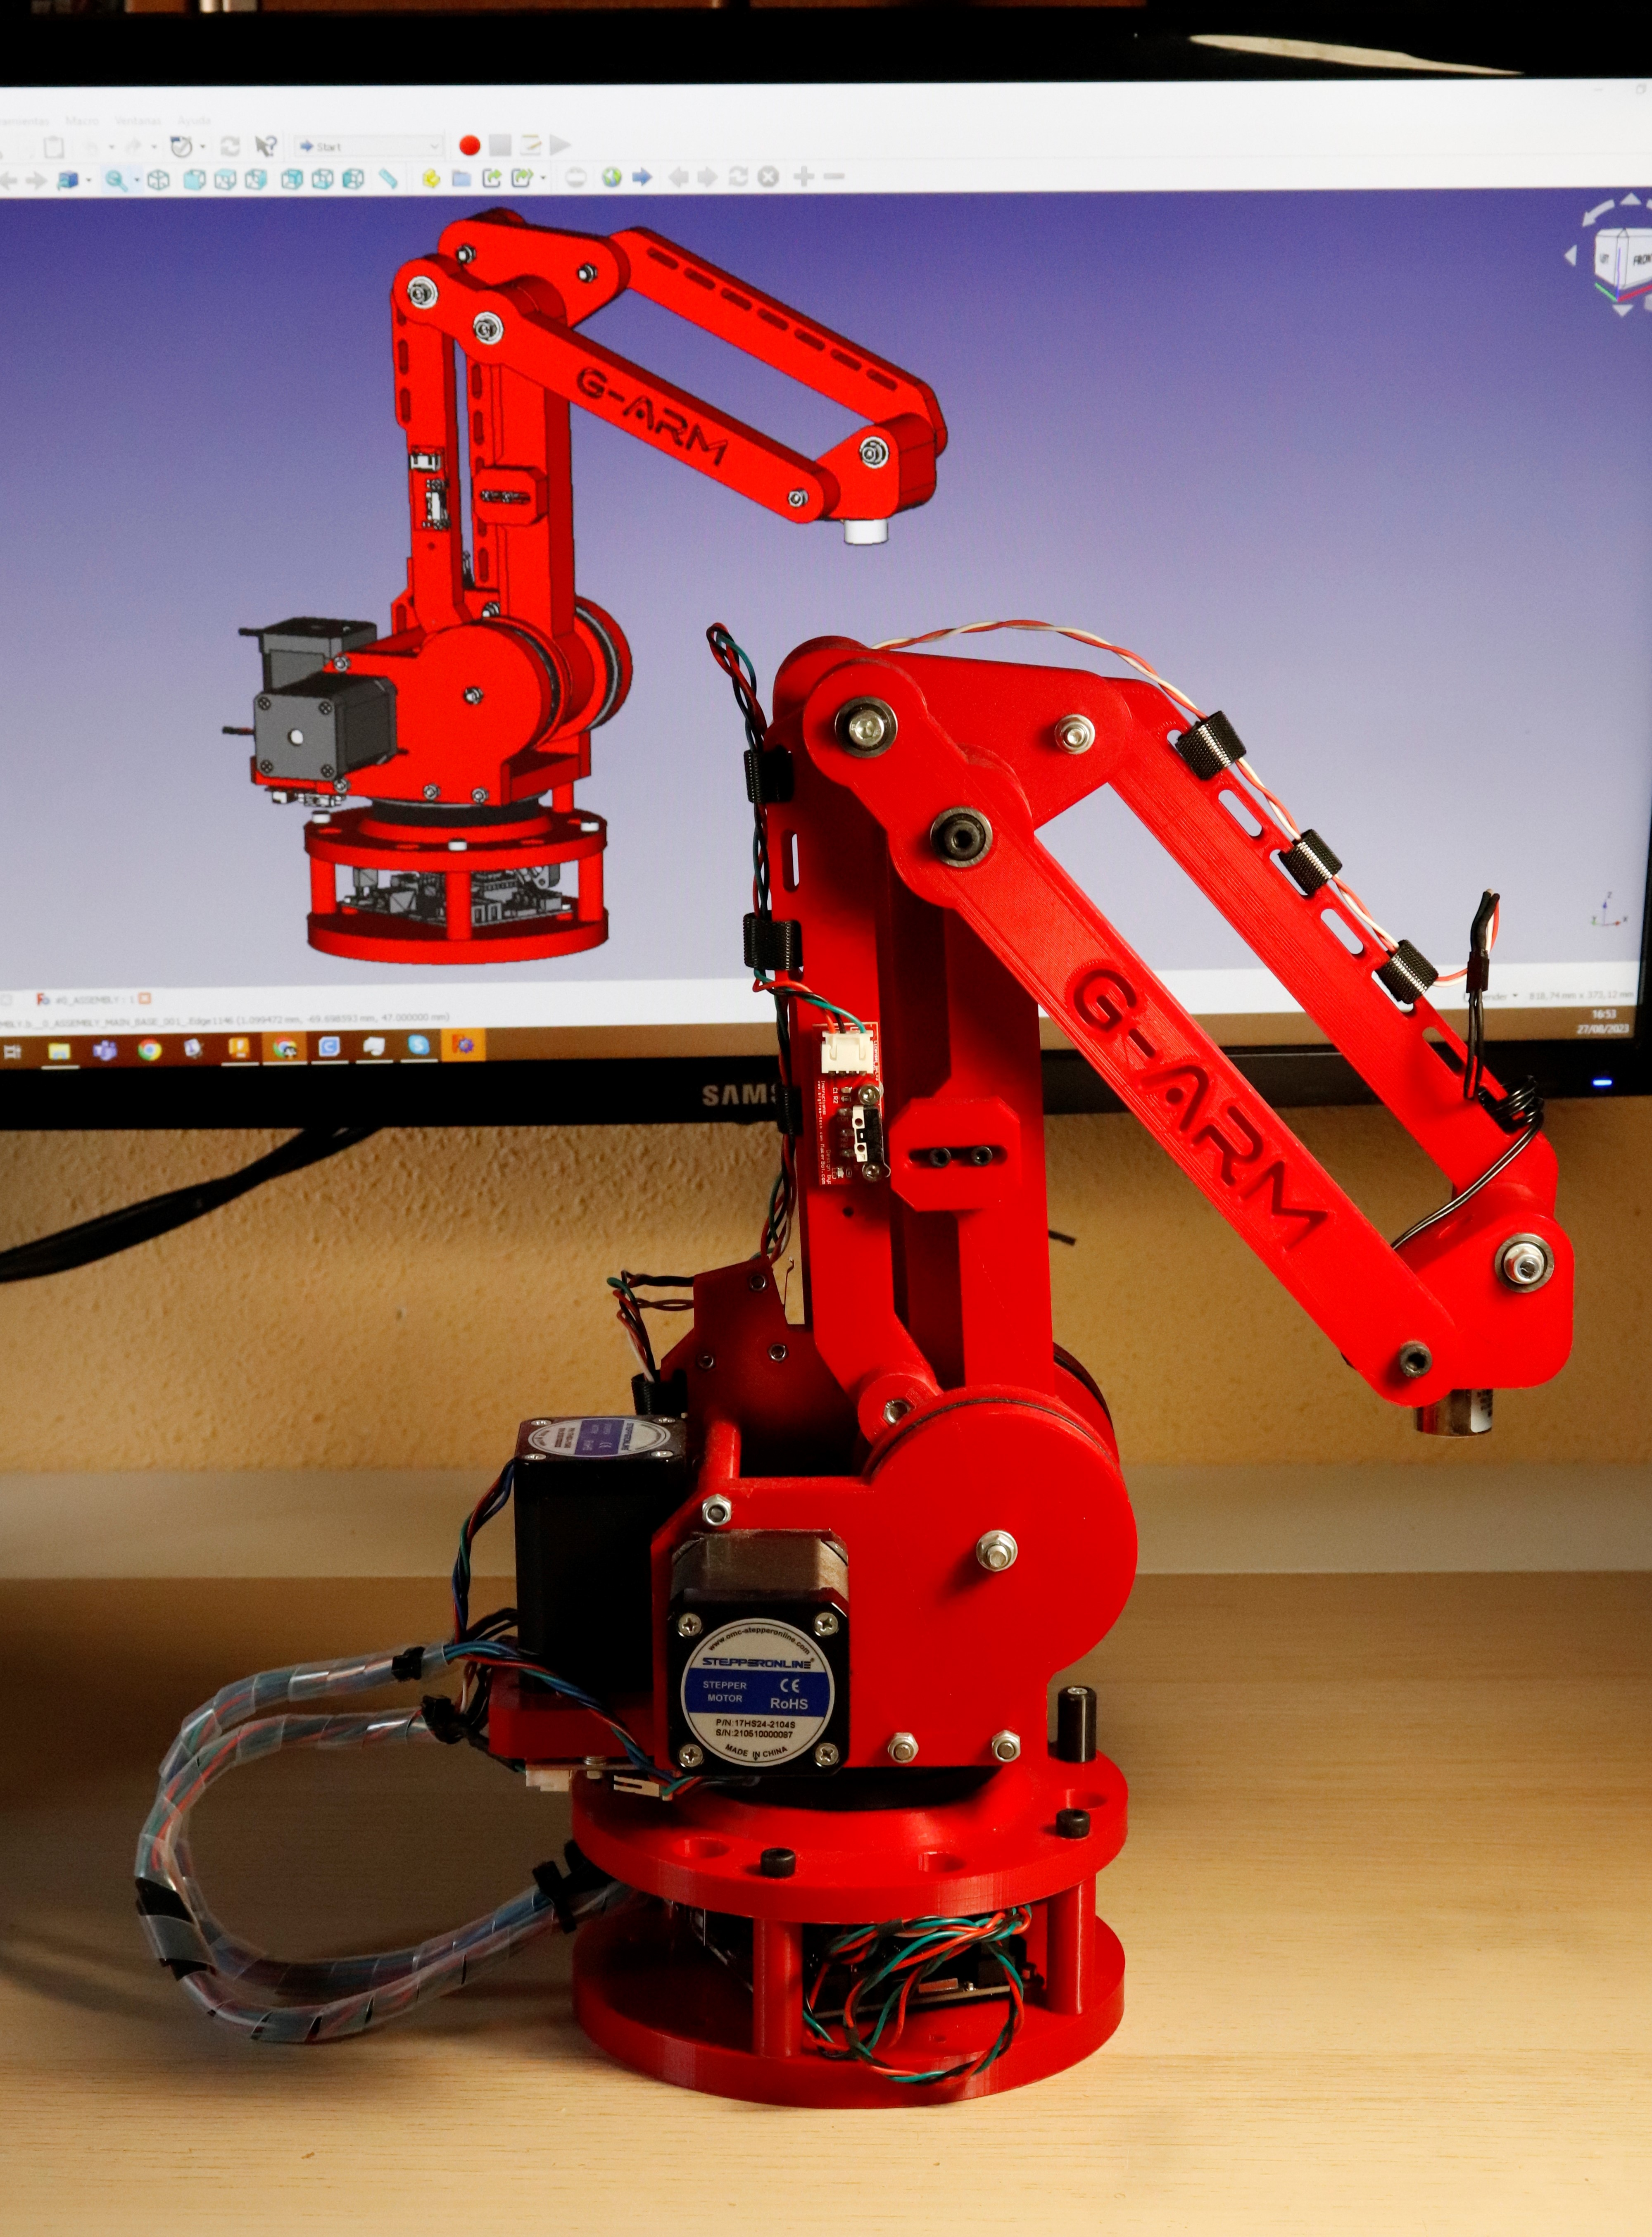
\includegraphics[width=14cm]{figs/montaje_real.jpg}
  \end{center}
  \caption{Montaje real del robot}
  \label{fig:montaje_real}
  \end{figure}\ 